\documentclass[letterpaper,10pt]{book}
\usepackage{hyperref}
\usepackage{natbib}
\usepackage{supertabular}
\usepackage{epsfig}
\usepackage{ifthen}
\usepackage{makeidx}
\usepackage{listings}
\usepackage{verbatim}
\usepackage{hyphenat}
\usepackage{ragged2e}

% Margins.
\setlength{\topmargin}{0mm}
\setlength{\textwidth}{160mm}
\setlength{\textheight}{230mm}
\setlength{\oddsidemargin}{0mm}
\setlength{\evensidemargin}{0mm}

% Names
\def\glc{{\sc Galacticus}}

% Physical constants.
\def\G{{\rm G}}
\def\clight{{\rm c}}
\def\d{{\rm d}}
\def\e{{\rm e}}

% CDM
\newcounter{CDMDone}
\setcounter{CDMDone}{0}
\def\CDM{\ifthenelse{\equal{\arabic{CDMDone}}{0}}{cold dark matter (CDM) \setcounter{CDMDone}{1}}{CDM}}

% CMB
\newcounter{CMBDone}
\setcounter{CMBDone}{0}
\def\CMB{\ifthenelse{\equal{\arabic{CMBDone}}{0}}{cosmic microwave background (CMB) \setcounter{CMBDone}{1}}{CMB}}

% IMF
\newcounter{IMFDone}
\setcounter{IMFDone}{0}
\def\IMF{\ifthenelse{\equal{\arabic{IMFDone}}{0}}{initial mass function (IMF) \setcounter{IMFDone}{1}}{IMF}}

% ISM
\newcounter{ISMDone}
\setcounter{ISMDone}{0}
\def\ISM{\ifthenelse{\equal{\arabic{ISMDone}}{0}}{interstellar medium (ISM) \setcounter{ISMDone}{1}}{ISM}}

% IGM
\newcounter{IGMDone}
\setcounter{IGMDone}{0}
\def\IGM{\ifthenelse{\equal{\arabic{IGMDone}}{0}}{intergalactic medium (IGM) \setcounter{IGMDone}{1}}{IGM}}

% ISCO
\newcounter{ISCODone}
\setcounter{ISCODone}{0}
\def\ISCO{\ifthenelse{\equal{\arabic{ISCODone}}{0}}{innermost stable circular orbit (ISCO) \setcounter{ISCODone}{1}}{ISCO}}

% SNe
\newcounter{SNeDone}
\setcounter{SNeDone}{0}
\def\SNe{\ifthenelse{\equal{\arabic{SNeDone}}{0}}{supernovae (SNe) \setcounter{SNeDone}{1}}{SNe}}

\makeindex

\begin{document}

\lstset{language=[95]Fortran}

\frontmatter

\pagestyle{empty}
\begin{center}
\begin{minipage}{7cm}
\begin{verbatim}
             ##                                     
  ####        #                  #                  
 #   #        #             #                       
#       ###   #  ###   ### ###  ##   ### ## ##   ## 
#       #  #  #  #  # #  #  #    #  #  #  #  #  #   
#   ###  ###  #   ### #     #    #  #     #  #   #  
 #   #  #  #  #  #  # #     #    #  #     #  #    # 
  ####  #### ### ####  ###   ## ###  ###   #### ##  

\end{verbatim}
\end{minipage}
\newline
A semi-analytic galaxy formation code.\\

\copyright\ 2009-2010, Andrew Benson
\end{center}

\tableofcontents

\mainmatter

\part{Installation and Basic Use}

\chapter{About Galacticus}

\glc\ is a semi-analytic model of galaxy formation. It solves equations describing how galaxies evolve in a merging hierarchy of dark matter halos in a cold dark matter universe. \glc\ has much in common with other semi-analytic models, such as the range of physical processes included and the type of quantities that it can predict.

In designing \glc\ our main goal was to make the code flexible, modular and easily extensible. Much greater priority was placed on making the code easy to use and modify than on making it fast. We believe that a modular and extensible nature is crucial as galaxy formation is an evolving science. In particular, key design features are:
\begin{description}
 \item [Extensible methods for all functions:] Essentially all functions within \glc\ are designed to be extensible, meaning that you can write your own version and insert it into \glc\ easily. For example, suppose you want to use an improved functional form for the \CDM\ halo mass function. You would simply write a subroutine conforming to a specified template that computes this mass function and add a short directive (see \S\ref{sec:CodeDirectives}) in your code which explains to the build system how to insert this function in \glc. A recompile of the code will then incorporate your new function.

 \item [Extensible components for tree nodes:] The basic structure in \glc\ is a merger tree, which consists of a linked tree of nodes which have various properties. \glc\ works by evolving the nodes forwards in time subject to a collection of differential equations and other rules. Each node can contains an arbitrary number of \emph{components}. A component may be a dark matter halo, a galactic disk, a black hole etc. Each component may have an arbitrary number of \emph{properties} (some of which may be evolving, others of which can be fixed). \glc\ makes it easy to add additional components. For example, suppose you wanted to add a ``stellar halo'' components (consisting of stars stripped from satellite galaxies). To do this, you would write a module which specifies the following for this component:
 \begin{itemize}
  \item Number of properties;
  \item Interfaces to set and get property values and rates of change;
  \item ``Pipes'' which allow for flows of mass/energy/etc. from one component to another;
  \item Routines describing the differential equations which govern the evolution of the properties;
  \item Routines describing how the component responds to various events (e.g. the node becoming a satellite, a galaxy-galaxy merger, etc.);
  \item Auxhiliary routines for handling outputs etc.
 \end{itemize}
 Short directives embedded in this module explain to the \glc\ build system how to incorporate the new component. A recompile will then build your new component into \glc. Typically, a new component can be created quickly by copying an existing one and modifying it as necessary. Furthermore, multiple implementations of a component are allowed. For example, \glc\ contains a component which is a Hernquist spheroid. You could add a de Vaucouler's spheroid component. A simple input parameter then allows you to select which implementation will be used in a given run.

 \item [Centralized ODE solver:] \glc\ evolves nodes in merger trees by calling an ODE solver which integrates forwards in time to solve for the evolution of the properties of each component in a node. This means that you do not need to provide explicit solutions for ODEs (in many cases such solutions are not available anyway) and timestepping is automatically handled to achieve a specified level of precision. The ODE solver allows for the evolution to be interrupted. A component may trigger an interrupt at any time and may do so for a number of reasons. A typical use is to actually create a component within a given node---for example when gas first begins to cool and inflow in a node the disk component must be created. Other uses include interrupting evolution when a merging event occurs.
\end{description}

\chapter{Installation}

\section{Required Libraries and Tools}

We run \glc\ on \href{http://fedoraproject.org/}{Fedora} Linux primarily. Installation instructions below are general, but we give some examples that are specific to Fedora (they probably work on other \href{http://yum.baseurl.org/}{{\tt yum}}-based Linux distributions though). For other distributions/OSs you'll need to figure out how to install pre-built packages or else install from source.

\begin{description}
 \item [Perl] The Perl language is a part of every Linux distribution that we know of, so use whatever method your distribution prefers to install it if you don't already have it. On Fedora the following (as root) will install Perl:
\begin{verbatim}
yum install perl perl-CPAN
\end{verbatim}
 If you need to install from source visit \href{http://www.perl.org/}{\tt http://www.perl.org/} and follow the instructions given there. We currently use Perl v5.10.0. \glc\ requires some Perl modules which probably are not installed by default. We recommend that you install these via \href{http://www.cpan.org/}{CPAN} (which probably is installed by default). The following modules should be installed.
 \begin{description}
  \item [\href{http://search.cpan.org/~kstephens/Data-Match-0.06/lib/Sort/Topological.pm}{{\tt Sort::Topological }}] This module implements dependency based sort and is used by the \glc\ build system to ensure that tasks are performed in the correct order. It can be installed using
\begin{verbatim}
perl -MCPAN -e 'install Sort::Topological'
\end{verbatim}
  \item [\href{http://search.cpan.org/~andrewf/LaTeX-Encode-0.03/lib/LaTeX/Encode.pm}{{\tt LaTeX::Encode }}] This module formats text for output to a \LaTeX\ document. It can be installed using
\begin{verbatim}
perl -MCPAN -e 'install LaTeX::Encode'
\end{verbatim}
  \item [\href{http://search.cpan.org/~grantm/XML-Simple-2.18/lib/XML/Simple.pm}{{\tt XML::Simple}}] Provides a simple interface in Perl for processing XML files. It is used extensively by \glc\ for building the code and for handling various data files. On Fedora the following (as root) will install {\tt XML::Simple}:
\begin{verbatim}
yum install perl-XML-Simple
\end{verbatim}
Alternatively, it can be installed from CPAN using:
\begin{verbatim}
perl -MCPAN -e 'install XML::Simple'
\end{verbatim}
  \item [\href{http://search.cpan.org/~sbeck/Math-SigFigs-1.09/lib/Math/SigFigs.pod}{{\tt Math::SigFigs}}] Provides formatting of numbers to a given number of significant figures. It is used by \glc\ when making plots. It can be installed from CPAN using:
\begin{verbatim}
perl -MCPAN -e 'install Math::SigFigs'
\end{verbatim}
  \item [\href{http://search.cpan.org/~djburke/Astro-Cosmology-0.90/Cosmology.pm}{{\tt Astro::Cosmology}}] Provides basic cosmological calculations. It is used by \glc\ when making plots to convert data points measured under the assumptions of one set of cosmological parameters to the cosmological parameters assumed by \glc. It can be installed from CPAN using:
\begin{verbatim}
perl -MCPAN -e 'force("install","Astro::Cosmology")'
\end{verbatim}

 \end{description}

\item[Gnuplot] The \href{http://www.gnuplot.info/}{\sc Gnuplot} plotting package is used extensively by \glc\ to produce plots. While not required for running \glc\ it is recommended as it allows you to easily check model results using the preexisting plotting scripts. On Fedora the following (as root) will install {\tt Gnuplot}:
\begin{verbatim}
yum install gnuplot
\end{verbatim}
Alternatively, {\sc Gnuplot} can be installed from source, following the online instructions.

\item[GraphViz] The \href{http://www.graphviz.org/}{GraphViz} package is used to create plots of merger tree structures. While not required to run \glc\ it is recommended to allow simple graphing of such structures (useful to get a visual impression of what's going on in the code). On Fedora the following (as root) will install GraphViz and a module that allows Perl to interact with it:
\begin{verbatim}
yum install graphviz perl-GraphViz
\end{verbatim}
Alternatively, GraphViz can be installed from source, following the online instructions, while the Perl module can be installed from CPAN using
\begin{verbatim}
perl -MCPAN -e 'install GraphViz'
\end{verbatim}

 \item [GNU Scientific Library] The \href{http://www.gnu.org/software/gsl/}{GNU Scientific Library} (GSL) is used extensively by \glc\ to perform numerous numerical functions. We currently use v1.13 of GSL---other versions may or may not work. On Fedora the following (as root) will install GSL:
\begin{verbatim}
yum install gsl gsl-devel
\end{verbatim}
Alternatively, GSL can be downloaded and installed from source as described online.

 \item [GNU Make] \glc\ uses \href{http://www.gnu.org/software/make/}{GNU Make} to build executables. Other implementations of {\tt make} may work, but we make no guarantees. On Fedora the following (as root) will install GNU Make:
\begin{verbatim}
yum install make
\end{verbatim}
Alternatively, GNU Make can be downloaded and installed from source as described online.

 \item [GFortran] \glc\ is written in Fortran using various aspects of the Fortran 2003 specification. We use \href{http://gcc.gnu.org/fortran/}{GNU Fortran} to compile \glc. You can use other Fortran compilers, but we make no claims as to whether they will support all required features of the Fortran language, or that they will produce correctly working code. On Fedora the following (as root) will install GNU Fortran:
\begin{verbatim}
yum install gcc-gfortran
\end{verbatim}
Alternatively, GNU Fortran can be downloaded and installed from source as described online. Note that \glc\ requires v4.4 or higher of {\tt gcc-gfortran}. On some systems (e.g. RHEL5) this is available in package {\tt gcc44-gfortran}.

 \item [FoX] \href{http://uszla.me.uk/space/software/FoX/}{FoX} is an XML parser for Fortran. The source can be downloaded from the link above. We recommend following the instructions provided with the download for install. We use FoX v4.0.4.

 \item [HDF5] The \href{http://hdf4.org/HDF5/}{HDF5} specification is used for storing output data from \glc. We currently use HDF5 v1.8.3. On Fedora the following (as root) will install the HDF5 libraries:
\begin{verbatim}
yum install hdf5 hdf5-devel
\end{verbatim}
Alternatively, HDF5 can be downloaded and installed from source. If this is done, we recommend the following build sequence:
\begin{verbatim}
 F9X=gfortran
 export F9X
 ./configure --prefix=/usr/local --enable-fortran --enable-production
 make
 make check
 make install
\end{verbatim}

 \item [FGSL] \href{http://www.lrz-muenchen.de/services/software/mathematik/gsl/fortran/}{FGSL} is a Fortran interface to the GNU Scientific Library and is used extensively by \glc. It can be downloaded from the link above. We use FGSL v0.9.2 and recommend the following build sequence. 
\begin{verbatim}
 ./configure --f90 gfortran
 make
 make install
\end{verbatim}

\end{description}

\section{Compiling Galacticus}

To build \glc\ (after installing all required libraries) ensure that you are in the {\tt Galacticus/v0.0.1} directory and then simply type:
\begin{verbatim}
 make Galacticus.exe
\end{verbatim}
This will create the {\tt Galactticus.exe} executable. The build takes some time, you'll see a set of XML files get created first which \glc\ uses to figure out how modules link in to the \glc\ code. After that, the Fortran files are compiled. We regularly build \glc\ using a parallel make without any problems.

The {\tt Makefile} contains a few options that you may want to adjust:
\begin{description}
 \item[{\tt F03COMPILER}] The command to invoke a Fortran 2003 compliant compiler. \glc\ should compile with any such compiler. In practice, we have only tried it using {\sc GFortran} v4.4. In particular, \glc\ makes use of certain Fortran 2003 features (notably procedure pointers and type-bound procedures) which older compilers might not handle (and some newer compilers might still have difficulty with);
 \item[{\tt PREPROCESSOR}] The command to invoke a preprocessor to handle {\tt \#IFDEF} etc. statements. We normally use {\tt cpp};
 \item[{\tt MODULETYPE}] A label identifying the structure of modules built by the compiler. This is used to detected when module interfaces have been changed (requiring a recompile of all dependent code) and when only the module internals have changed. When the {\sc GFortran} compiler is used {\tt GCC-f95-on-LINUX} should be used here. Look in {\tt ./scripts/build/Compare\_Module\_Files.pl} for other possibilities (if your compiler isn't listed you'll need to either edit that script or deal with longer recompiles if you edit the code).
 \item[{\tt F03FLAGS}] Flags to pass to the Fortran compiler. Standard options for both error-checking and optimized builds for the {\sc GFortran} compiler are given in the {\tt Makefile}.
\end{description}

\section{Installing Without Root Access}

It is possible to install \glc\ without root access to your computer. The following approach has worked in many cases---some adjustments may be required for your specific system. Depending on what is already installed on your system, you may be able to skip some of the following installs. (Or, alternatively, you may need to install additional tools.) Choose a location to install that has at least 4Gb of free space. In the following, this install location is referred to as {\tt /your/install/path}.

\lstdefinelanguage{simple}{morecomment=[l]!}
\begin{lstlisting}[language=simple,stringstyle=\ttfamily,commentstyle=\itshape]
! Install Perl local::lib for local installs of modules:

mkdir .cpan
mkdir perl5
ln -sf /your/install/path/.cpan $HOME/
ln -sf /your/install/path/perl5 $HOME/
wget http://search.cpan.org/CPAN/authors/id/M/MS/MSTROUT/local-lib-1.006000.tar.gz
tar xvfz local-lib-1.006000.tar.gz 
cd local-lib-1.006000
perl Makefile.PL --bootstrap
make
make test
make install
perl -I$HOME/perl5/lib/perl5 -Mlocal::lib >> $HOME/.cshrc

! Install Perl modules:

perl -MCPAN -e "install Sort::Topological"
perl -MCPAN -e "install LaTeX::Encode"
perl -MCPAN -e "install XML::Simple"
perl -MCPAN -e "install Math::SigFigs"
perl -MCPAN -e "install GraphViz"
perl -MCPAN -e 'force("install","Astro::Cosmology")'

! Install GnuPlot:

wget "http://downloads.sourceforge.net/project/gnuplot/gnuplot/4.4.0/gnuplot-4.4.0.tar.gz"
tar xvfz gnuplot-4.4.0.tar.gz
cd gnuplot-4.4.0
./configure --prefix=/your/install/path
make
make install

! Install GraphViz:

wget "http://www.graphviz.org/pub/graphviz/stable/SOURCES/graphviz-2.26.3.tar.gz"
tar xvfz graphviz-2.26.3.tar.gz
cd graphviz-2.26.3
./configure --prefix=/your/install/path
make
make check
make install

! Install GSL:

wget "http://www.mirrorservice.org/sites/ftp.gnu.org/gnu/gsl/gsl-1.14.tar.gz"
tar xvfz gsl-1.14.tar.gz
cd  gsl-1.14
./configure --prefix=/your/install/path
make
make check
make install

! Install GFortran:

wget "ftp://ftp.gnu.org/gnu/gcc/gcc-4.4.4/gcc-4.4.4.tar.bz2"
tar xvfj gcc-4.4.4.tar.bz2
mkdir gcc-build
cd gcc-build
../gcc-4.4.4/configure --prefix=/your/install/path/gcc-trunk --enable-languages=c,c++,fortran --disable-multilib
make
make install

! Add to .cshrc (or equivalent):

setenv PATH /your/install/path:$PATH                                                                                           
setenv LD_LIBRARY_PATH /your/install/path/gcc-trunk/lib:/your/install/path/lib:$LD_LIBRARY_PATH                                                                     

! Install FGSL:

wget "http://www.lrz-muenchen.de/services/software/mathematik/gsl/fortran/fgsl-0.9.3.tar.gz"
tar xvfz fgsl-0.9.3.tar.gz
./configure --f90 gfortran --gsl /your/install/path
make
make install

! Install zlib:

wget "http://zlib.net/zlib-1.2.5.tar.gz"
tar xvfz zlib-1.2.5.tar.gz
cd zlib-1.2.5
./configure --prefix=/your/install/path
make
make check
make install

! Install HDF5:

wget http://www.hdfgroup.org/ftp/HDF5/current/src/hdf5-1.8.4-patch1.tar.bz2
tar xvfz hdf5-1.8.4-patch1.tar.bz2
cd hdf5-1.8.4-patch1
setenv F9X gfortran
./configure --prefix=/your/install/path --enable-fortran --enable-production --with-zlib=/your/install/path
make
make check
make install

! Install FoX:

wget "http://www.uszla.me.uk/FoX/source/FoX-4.0.4-full.tar.gz"
tar xvfz FoX-4.0.4-full.tar.gz
cd FoX-4.0.4
setenv FC gfortran
./configure --prefix=/your/install/path
make
make check
make install

! Install Bazaar:

wget "http://launchpad.net/bzr/2.2/2.2b3/+download/bzr-2.2b3.tar.gz"
tar xvfz bzr-2.2b3.tar.gz
python setup.py install --home /your/install/path

! Install Galacticus:

wget "http://www.ctcp.caltech.edu/galacticus/galacticus_v0.0.1.tar.bz2"
tar xvfj galacticus_v0.0.1.tar.bz2
cd Galacticus/v0.0.1

! Add to Makefile (below the F03FLAGS = line):

F03FLAGS += -fintrinsic-modules-path /your/install/path/finclude -fintrinsic-modules-path /your/install/path/include/gfortran -fintrinsic-modules-path /your/install/path -fintrinsic-modules-path /your/install/path/include -L /your/install/path/lib
\end{lstlisting}

It should then be possible to compile and run \glc.

\chapter{Running Galacticus}

\section{Parameter Files}

\glc\ requires a file of parameters to be given as a command line argument. (In fact, it technically doesn't as all of the parameters will be assigned default values if no file is given, but in most cases you want to change some parameters, in which case you must specify them in a file.) The parameter file is an XML file (which makes it easy to manipulate and construct these files from within many languages, e.g. Perl) with the following structure:
\begin{verbatim}
 <parameters>
   <parameter>
     <name>parameter1name</name>
     <value>parameter1value</value>
   </parameter>
   .
   .
   .
 </parameters>
\end{verbatim}
Each {\tt parameter} element contains {\tt name} and {\tt value} elements which contain the parameter name and desired value respectively. The value can be a number, word(s) or an array of space-separated numbers. Parameters are used to control the values of numerical parameters and also to select methods and other options. If a parameter is not specified in the file a default value (hard coded into \glc) will be used instead. The default values have been chosen to produce a realistic model of galaxy formation, but may change as \glc\ evolves.

All parameter values (both those specified in this file and those set to default) used during a \glc\ run are output to the {\tt Parameters} group within the \glc\ output file. The script {\tt scripts/aux/Extract\_Parameter\_File.pl} will, if given a \glc\ output file, extract the parameters from it and output them into an XML file suitable for re-input into \glc.

\section{Running Galacticus}

\glc\ is running using
\begin{verbatim}
 Galacticus.exe [<parameterFile>]
\end{verbatim}
where {\tt parameterFile} is the name of the file containing a list of parameter values for \glc. \glc\ will display messages indicating its progress as it runs (the verbosity can be controlled with the {\tt verbosityLevel} parameter).

\subsection{Restarting A Crashed Run}

If \glc\ crashes, it can be useful to restart the calculation from just prior to the crash to speed the debugging process. \glc\ has functionality to store and retrieve the internal state of any modules and to recover this to permit such restarting. Currently, this is implemented with the {\tt build} method of merger tree construction, such that the internal state is stored prior to commencing the building of each tree, thereby allowing a calculation to be restarted with the tree that crashed. More general store/retrieve behavior is planned for future releases.

To cause \glc\ to periodically store its internal state include the following input parameter:
\begin{verbatim}
  <parameter>
    <name>stateFileRoot</name>
    <value>galacticusState</value>
  </parameter>
\end{verbatim}
This will cause the internal state to be stored to files {\tt galacticusState.state} and {\tt galacticusState.fgsl.state} prior to commencing building each merger tree. Should a tree crash then replace this input parameter with:
\begin{verbatim}
  <parameter>
    <name>stateRetrieveFileRoot</name>
    <value>galacticusState</value>
  </parameter>
  <parameter>
    <name>mergerTreeBuildTreesBeginAtTree</name>
    <value>N</value>
  </parameter>
\end{verbatim}
where {\tt N} is the number of the tree that crashed. This will cause calculations to begin with tree {\tt N} and for the internal state to be recovered from the above mentioned files. The resulting tree and all galaxy formation calculations should therefore proceed just as in the original run (and so create the same crash condition).

\chapter{Input Parameters}

The following is an alphnumerically sorted list of all input parameters defined in \glc. Each parameter is listed by name, along with a description, default value (if one is specified in \glc), the file and program unit with which it is associated. Where relevant, references for parameters and the default values are given.

\input{dataParameters}

\chapter{Extracting and Analyzing Results}

\glc\ stores its output in an \href{http://www.hdfgroup.org/HDF5/}{HDF5} file. The contents of this file can be viewed and manipulated using a variety of ways including:
\begin{description}
 \item[\href{http://www.hdfgroup.org/hdf-java-html/hdfview/}{{\sc HDFView}}] This is a graphical viewer for exploring the contents of HDF5 files;
 \item[\href{http://www.hdfgroup.org/products/hdf5_tools/index.html\#h5dist}{HDF5 Command Line Tools}] A set of tools which can be used to extract data from HDF5 files (\href{http://www.hdfgroup.org/HDF5/doc/RM/Tools.html#Tools-Dump}{{\tt h5dump}} and \href{http://www.hdfgroup.org/HDF5/doc/RM/Tools.html#Tools-Ls}{{\tt h5ls}} are particularly useful);
 \item[\href{http://www.hdfgroup.org/HDF5/doc/RM/RM_H5Front.html\#F90andCPPlus}{C++ and Fortran 90 APIs}] Allow access to and manipulation of data in HDF5 files;
 \item[\href{http://code.google.com/p/h5py/}{{\sc h5py}}] A Python interface to HDF5 files.
\end{description}

In the remainder of this section the structure of \glc\ HDF5 files is described and a general-purpose Perl module which we use to extract data in a convenient manner is outlined.

\section{General Structure of Output File}

Figure~\ref{fig:glcOutputFileStructure} shows the structure of a typical \glc\ output file. The various groups and subgroups are described below.

\begin{figure}
\begin{center}
\begin{verbatim}
outputFile.hdf5
 |
 +-> Outputs                                  Group
 |    |
 |    +-> Output1                             Group
 |    |    |
 |    |    +-> mergerTree1                    Group
 |    |    |     |
 |    |    |     +-> nodeProperty1            Dataset {1002/Inf}
 |    |    |     +-> ...                      Dataset {1002/Inf}
 |    |    |     +-> ...                      Dataset {1002/Inf}
 |    |    |     +-> ...                      Dataset {1002/Inf}
 |    |    |     +-> nodePropertyN            Dataset {1002/Inf}
 |    |    |
 |    |    x-> ...                            Group
 |    |    x-> ...                            Group
 |    |    x-> ...                            Group
 |    |    x-> mergerTreeN                    Group
 |    |    |
 |    |    +-> outputExpansionFactor          Dataset {1}
 |    |    +-> outputTime                     Dataset {1}
 |    |
 |    x-> Output2                             Group
 |
 +-> Parameters                               Group
 |    |
 |    +-> inputParameter1                     Dataset {1}
 |    +-> ...                                 Dataset {1}
 |    +-> ...                                 Dataset {1}
 |    +-> ...                                 Dataset {1}
 |    +-> inputParameterN                     Dataset {1}
 |
 +-> Version                                  Group
 |    |
 |    +-> runTime                             Dataset {1}
 |    +-> versionMajor                        Dataset {1}
 |    +-> versionMinor                        Dataset {1}
 |    +-> versionRevision                     Dataset {1}
 |
 +-> globalHistory                            Group
      |
      +-> historyExpansion                    Dataset {30}
      +-> historyStarFormationRate            Dataset {30}
      +-> historyTime                         Dataset {30}
\end{verbatim}
\end{center}
\caption{Structure of a \glc\ HDF5 output file.}
\label{fig:glcOutputFileStructure}
\end{figure}

\subsection{Parameters}

The {\tt Parameters} group contains a record of all parameter values (either input or default) that were used for this \glc\ run. The group contains a long list of datasets, each dataset named for the corresponding parameter and with a single entry giving the value of that parameter. The {\tt scripts/aux/Extract\_Parameter\_File.pl} script can be used to extract these parameter values to an XML file suitable for re-input into \glc.

\subsection{Version}

The {\tt Version} group contains a record of the \glc\ version used for this model, storing the major and minor version numbers and the revision number. Additionally, the time at which the model was run is stored.

\subsection{globalHistory}

The {\tt globalHistory} group stores volume averaged properties of the model universe as a function of time. Currently, the properties stored are:
\begin{description}
 \item[{\tt historyTime}] Cosmic time (in Gyr);
 \item[{\tt historyExpansion}] Expansion factor;
 \item[{\tt historyStarFormationRate}] Volume averaged star formation rate (in $M_\odot/$Gyr/Mpc$^3$).
\end{description}

\subsection{Outputs}

The {\tt Outputs} group contains one or more sub-groups corresponding to the output times requested from \glc. Each sub-group contains the following information:
\begin{description}
 \item[{\tt outputTime}] The cosmic time (in Gyr) at this output;
 \item[{\tt outputExpansionFactor}] The expansion factor at this output;
 \item[{\tt mergerTree} subgroups] A set of {\tt mergerTree} groups as described below.
\end{description}

\subsubsection{mergerTree subgroups}

Each {\tt mergerTree} subgroup contains all data on a single merger tree. The group consists of a collection of datasets each of which lists a property of all nodes in the tree which exist at the output time. Additionally, the {\tt volumeWeight} dataset gives the weight (in Mpc$^{-3}$) which should be assigned to this tree (and all nodes in it) to create a volume-averaged sample.

\subsection{Optional Outputs}

Numerous other quantities can be optionally output. These are documented below:

\subsubsection{Mass Accretion Histories}

A mass accretion history (i.e. mass as a function of time) for the main branch in each merger tree can be output by setting {\tt massAccretionHistoryOutput}$=${\tt true}. If requested, a new group {\tt massAccretionHistories} will be made in the \glc\ output file. It will contain groups called {\tt mergerTreeN} where {\tt N} is the merger tree index. Each such group will contain the following three datasets, defined for the main branch of the tree\footnote{``Main branch'' is defined by starting from the root node of a tree and repeatedly stepping back to the most massive progenitor of the branch. This does not necessarily pick out the most massive progenitor at a given time.}:
\begin{description}
 \item [{\tt nodeIndex}] The index of the node in the tree;
 \item [{\tt nodeTime}] The time at this point in the tree (in Gyr);
 \item [{\tt nodeMass}] The mass of the node at this point in the tree (in $M_\odot$).
\end{description}

\subsubsection{Pre-Evolution Merger Trees}

\glc\ can output the full structure of merger trees prior to any evolution. Merger tree structure can be requested by setting {\tt mergerTreeStructureOutput}$=${\tt true}. Structures are written to a new group, {\tt mergerTreeStructures}, in the \glc\ output file. This group will contain groups called {\tt mergerTreeN} where {\tt N} is the merger tree index. Each such group will contain the following datasets:
\begin{description}
 \item [{\tt nodeIndex}] The index of the node in the tree;
 \item [{\tt childNodeIndex}] The index of this node's first child node;
 \item [{\tt parentNodeIndex}] The index of this node's parent node;
 \item [{\tt siblingNodeIndex}] The index of this node's sibling node;
 \item [{\tt nodeTime}] The time at this point in the tree (in Gyr);
 \item [{\tt nodeMass}] The mass of the node at this point in the tree (in $M_\odot$).
\end{description}
Additional, optional, datasets can be added by setting appropriate input parameters. Currently these include:
\begin{itemize}
 \item [Virial quantities] If {\tt mergerTreeStructureOutputVirialQuantities}$=${\tt true} then two additional datasets are included:
 \begin{description}
  \item [{\tt nodeVirialRadius}] The virial radius of the node (in Mpc);
  \item [{\tt nodeVirialVelocity}] The virial velocity of the node (in km/s);
 \end{description}
 \item [Dark matter scale radii] If {\tt mergerTreeStructureOutputDarkMatterScaleRadius}$=${\tt true} then an additional dataset is included:
 \begin{description}
  \item [{\tt darkMatterScaleRadius}] The scale radius of this node's dark matter halo profile (in Mpc);
 \end{description}
\end{itemize}

\section{Perl Module for Data Extraction}

A Perl module is provided that allows for easy extraction of datasets from the \glc\ output file together with a straightforward way to implement derived properties. To use this Perl module, add
\begin{verbatim}
 use lib "./perl";
 use PDL;
 use Galacticus::HDF5;
\end{verbatim}
at the start of your Perl script. The {\tt Galacticus::HDF5} module will import data from a \glc\ HDF5 file into PDL variables. All data are stored in a single structure, which also specifies the file, output and range of trees to read. An example of reading a dataset from a file is:
\begin{verbatim}
 $dataSet{'file'} = "galacticus.hdf5";
 $dataSet{'output'} = 1;
 $dataSet{'tree'} = "all";
 $dataSet{'dataRange'} = [1,2];
 $dataSet{'store'} = 0;
 &HDF5::Get_Dataset(\%dataSet,['nodeMass']);
 $dataSets = \%{$dataSet{'dataSets'}};
 print ${$dataSets->{'nodeMass'}}."\n";
\end{verbatim}
The {\tt \%dataSet} hash is initialized with information to specify which file, output and trees should be used. Its settable components are:
\begin{description}
 \item [{\tt file}] The name of the \glc\ output file to be read.
 \item [{\tt output}] Specify the output number in the file which should be read.
 \item [{\tt tree}] Specify the tree which should be read, or use ``all'' to specify that all trees be read.
 \item [{\tt dataRange}] Gives the first and last entry in the dataset to read---this facilitates reading of partial datasets (and therefore reading datasets in a piecemeal fashion). If this component is missing, the entire dataset is read.
 \item[{\tt store}] If set to 1, any derived properties will be stored back in the \glc\ output file for later retrieval. If set to 0 (or if this option is not present), derived properties will not be stored. Currently, storing of derived properties in the \glc\ file is only possible if the {\tt tree} option is set to ``all'' and no {\tt dataRange} is specified.
\end{description}
The {\tt \&HDF5::Get\_Dataset($\backslash$\%dataSet,['nodeMass']);} call requests that the {\tt nodeMass} dataset be read. It is return as a PDL variable in the {\tt nodeMass} element of the {\tt dataSets} hash which is itself a member of {\tt \$dataSet}. The final lines in the example simply write out the resulting array of {\tt nodeMass} values.

\subsection{Derived Properties}

Derived properties can be created by giving defining functions along with a regular expression string that allows them to be matched. For example, the {\tt Galacticus::Baryons} module implements a hot gas fraction property called {\tt hotHaloFraction} or {\tt hotHaloFrac}. It has the following form:
\begin{verbatim}
package Baryons;
use PDL;
use Galacticus::HDF5;
use Data::Dumper;

%HDF5::galacticusFunctions = ( %HDF5::galacticusFunctions,
    "hotHalo(Fraction|Frac)" => "Baryons::Get_hotHaloFraction"
    );

my $status = 1;
$status;

sub Get_hotHaloFraction {
    $dataSet = shift;
    $dataSetName = $_[0];
    &HDF5::Get_Dataset($dataSet,['hotHaloMass','nodeMass']);
    $dataSets = \%{${$dataSet}{'dataSets'}};
    ${$dataSets->{$dataSetName}} = ${$dataSets->{'hotHaloMass'}}/${$dataSets->{'nodeMass'}};
}

\end{verbatim}
The module begins by adding an entry to the {\tt \%HDF5::galacticusFunctions} hash. The key gives a regular expression which matches to the name of the property to be defined. The value of the key gives the name of a subroutine to be called to evaluate this expression. The subroutine is defined below. When called, it receives the {\tt \$dataSet} structure along with the name of the requested property. The subroutine should then simply evaluate the requested property and store it in the appropriate location within {\tt \$dataSet}. Note that the subroutine can request additional datasets be loaded (as happens above where {\tt hotHaloMass} and {\tt nodeMass} are requested) if they are needed for its calculations.

\subsubsection{Available Derived Properties}

\begin{description}
 \item[{\tt hotHalo(Fraction\textbar Frac)}] The fraction the node's mass in the hot gas halo. Provided by: {\tt Galacticus::Baryons}.
 \item[{\tt inclination}] A randomly selected inclination for the disk (in degrees). Provided by: {\tt Galacticus::Inclination}.
 \item[{\tt \textasciicircum(disk\textbar bulge)StellarLuminosity:.*:dustAtlas($\backslash$[faceOn$\backslash$])\$}] Dust-extingiushed luminosities for disk and bulge found by interpolating in the dust tables of \cite{ferrara_atlas_1999}. If the {\tt [faceOn]} qualifier is present, extinctions are computed assuming that the disk is observed face-on, otherwise a random inclination is used. Optionally, the dust atlas file to used can be specified via {\tt \$\{\$dataSet\}\{'dustAtlasFile'\}}. The available dust atlases span a limited range of spheroid sizes and central optical depths in their tabulations. Standard behavior is to extrapolate beyond the ends of these ranges. This can be controlled via {\tt \$\{\$dataSet\}\{'dustAtlasExtrapolateInSize'\}} and {\tt \$\{\$dataSet\}\{'dustAtlasExtrapolateInTau'\}} respectively, which can be set to {\tt yes}/{\tt no} (or, equivalently, 1/0). Provided by: {\tt Galacticus::DustAttenuation}.
 \item[{\tt \textasciicircum magnitude([\textasciicircum :]+):([\textasciicircum :]+):([\textasciicircum :]+):z([$\backslash$d$\backslash$.]+)(:dust[\textasciicircum :]+)?(:vega\textbar :AB)?}] Absolute magnitude corresponding to a stellar luminosity, in either Vega or AB systems. Provided by: {\tt Galacticus::Magnitudes}.
\end{description}

\chapter{Input Data}

In some configurations, \glc\ requires additional input data to run. For example, if asked to process galaxy formation through a set of externally derived merger trees, then a file describing those trees must be given. In the remainder of this section we describe the structure of external datasets which can be inputs to \glc.

\section{Broadband Filters}\index{filters!broadband}

To compute luminosities through a given filter, \glc\ requires the response function, $R(\lambda)$, of that filter to be defined. \glc\ follows the convention of \cite{hogg_k_2002} in defining the filter response to be the fraction of incident photons received by the detector at a given wavelength, multiplied by the relative photon response (which will be 1 for a photon-counting detector such as a CCD, or proportional to the photon energy for a bolometer/calorimeter type detector. Filter response files are stored in {\tt data/filters/}. Their structure is shown below, with the {\tt SDSS\_g.xml} filter reponse file used as an example:
\begin{verbatim}
 <filter>
  <description>SDSS g vacuum (filter+CCD +0 air mass)</description>
  <name>SDSS g</name>
  <origin>Michael Blanton</origin>
  <response>
    <datum>   3630.000      0.0000000E+00</datum>
    <datum>   3680.000      2.2690000E-03</datum>
    <datum>   3730.000      5.4120002E-03</datum>
    <datum>   3780.000      9.8719997E-03</datum>
    <datum>   3830.000      2.9449999E-02</datum>
    .
    .
    . 
  </response>
  <effectiveWavelength>4727.02994472695</effectiveWavelength>
  <vegaOffset>0.107430167298754</vegaOffset>
</filter>
\end{verbatim}
The {\tt description} tag should provide a description of the filter, while the {\tt name} tag provides a shorter name. The {\tt origin} tag should describe from where/whom this filter originated. The {\tt response} element contains a list of {\tt datum} tags each giving a wavelength (in Angstroms) and response pair. The normalization of the response is arbitrary. The {\tt effectiveWavelength} tag gives the mean, response-weighted wavelength of the filter and is used, for example, in dust attenuation calculations. The {\tt vegaOffset} tag gives the value (in magnitudes) which must be added to an AB-system magnitude in this system to place it into the Vega system. Both {\tt effectiveWavelength} and {\tt vegaOffset} can be computed by running
\begin{verbatim}
 scripts/filters/vega_offset_effective_lambda.pl data/filters
\end{verbatim}
which will compute these values for any filter files that do not already contain them and append them to the files.

\section{Merger Trees}\label{sec:MergerTreeFiles}

While \glc\ can build merger trees using analytic methods it is often usedful to be able to utilize merger trees from other sources (e.g. extracted from an N-body simulation). To facilitate this, \glc\ allows merger trees to be read from an HDF5 files. To do so, set the {\tt [mergerTreeConstructMethod]} input parameter to {\tt read} and specify the filename to read via their {\tt [mergerTreeReadFileName]} parameter.

The HDF5 file should have the following structure:
\begin{verbatim}
mergerTreeFile.hdf5 {
  [mergerTrees] {
    [mergerTree1] {
      volumeWeight => (1)
      treeIndex    => (1)
      nodeIndex    => (nodeCount1)
      parentNode   => (nodeCount1)
      childNode    => (nodeCount1)
      siblingNode  => (nodeCount1)
      nodeMass     => (nodeCount1)
      nodeRedshift => (nodeCount1)
    }
    [mergerTree2] {
      volumeWeight => (1)
      treeIndex    => (1)
      nodeIndex    => (nodeCount2)
      parentNode   => (nodeCount2)
      childNode    => (nodeCount2)
      siblingNode  => (nodeCount2)
      nodeMass     => (nodeCount2)
      nodeRedshift => (nodeCount2)
    }
    .
    .
    .
  }
}
\end{verbatim}
where {\tt volumeWeight} is the number of such trees per unit volume, {\tt treeIndex} is an index for this tree, {\tt nodeIndex} is a unique integer identifier for their node, {\tt parentNode} is the index of the parent node (or $-1$ if none exists), {\tt childNode} is the index of the most massive child node (or $-1$ if none exists), {\tt siblingNode} is the index of the sibling node (or $-1$ if none exists), {\tt nodeMass} is the mass of the nodeCount1 (in $M_\odot$) and {\tt nodeRedshift} is the redshift at which the node exists. Here, {\tt nodeCount1} is the number of nodes in tree number 1 for example. The trees must be self-consistent (i.e. parent and child indices must make sense, sibling should all have the same parent, parents must exist at lower redshift than their children, there must be a unique root to the tree).

An example of how to construct such a file is given by the {\tt scripts/aux/Millennium\_Trees\_Grab.pl} script which pulls merger tree data from the Millennium Simulation database and outputs it as an HDF5 file in the format required by \glc. This script is used as follows:
\begin{verbatim}
 scripts/aux/Millennium_Trees_Grab.pl --output <outputFile> --user <userName> --password <password> --select <sqlSelection>
\end{verbatim}
All arguments are optional. If present the {\tt user} and {\tt password} will be used to log in to the database server. Merger trees are output to the file specified by {\tt output} if present, or to {\tt Millennium\_Trees.hdf5} otherwise. If the {\tt select} keyword is present, then its contents are added to the SQL query sent to the database and permits you to select subsamples of merger trees (e.g. those in a given mass range). The script {\tt examples/Millennium\_Trees\_Grab.csh} shows an example of how this script should be used.

\part{Physical Implementation}

In this Part we describe the physical implementation of galaxy formation in \glc, including all components and their properties and additional output quantities from the code.

\chapter{Node Components}

\section{(Supermassive) Black Hole}

\subsection{``Null'' Implementation}

The null black hole implementation defines the same properties as all other black hole implementations, but sets the methods to point to dummy routines (for rate adjustment and derivative computation) or to {\tt null()} for get/set methods. It can be used to effectively switch off black holes. Of course, this is safe only if none of the other active components expect to get or set black hole properties (or if they rely on a sensible implementation of black hole evolution).

\subsection{``Standard'' Implementation}

\subsubsection{Properties}

The standard black hole implementation defines the following properties:
\begin{description}
 \item [{\tt Black\_Hole\_Mass}] The mass of the black hole: $M_\bullet$ {\tt [blackHoleMass]}.
 \item [{\tt Black\_Hole\_Spin}] The spin of the black hole, $j_\bullet$ {\tt [blackHoleSpin]}.
\end{description}

\subsubsection{Initialization}

Black holes are not initialized, they are created (with a seed mass given by {\tt blackHoleSeedMass} and zero spin) as needed.

\subsubsection{Differential Evolution}

In the standard black implementation the mass and spin evolve as:
\begin{eqnarray}
\dot{M}_\bullet &=& (1-\epsilon_{\rm radiation}) \dot{M}_0 \\
\dot{j}_\bullet &=& \dot{j}(M_\bullet,j_\bullet,\dot{M}_0),
\end{eqnarray}
where $\dot{M}_0$ is the rest mass accretion rate, $\epsilon_{\rm radiation}$ is the radiative efficiency of the accretion flow feeding the black hole and $\dot{j}(M_\bullet,j_\bullet,\dot{M}_0)$ is the spin-up function of that accretion flow (see \S\ref{sec:AccretionDisks}). The rest mass accretion rate is computed assuming Bondi-Hoyle-Lyttleton accretion from the spheroid gas reservoir (with an assumed temperature of {\tt bondiHoyleAccretionTemperature}) enhanced by a factor of {\tt bondiHoyleAccretionEnhancement}. The rest mass accretion rate is removed (as a mass sink) from the spheroid component.

\subsubsection{Event Evolution}

\noindent\emph{Node mergers:} None.\\

\noindent\emph{Satellite merging:} The black holes in the two merging galaxies are instantaneously merged. Properties are computed using the selected black hole binary merger method (see \S\ref{sec:BlackHoleBinaryMergers}).\\

\noindent\emph{Node promotion:} None.\\

\section{Hot Halo}

\subsection{``Null'' Implementation}

The null hot halo implementation leaves all methods to point to dummy routines (for rate adjustment and derivative computation) or to {\tt null()} for get/set methods. It can be used to effectively switch off hot halos. Of course, this is safe only if none of the other active components expect to get or set hot halo properties (or if they rely on a sensible implementation of hot halo evolution).

\subsection{``Standard'' Implementation}

\subsubsection{Properties}

The standard hot halo implementation defines the following properties:
\begin{description}
 \item [{\tt Hot\_Halo\_Unaccreted\_Mass}] The mass of gas in the hot halo: $M_{\rm failed}$.
 \item [{\tt Hot\_Halo\_Mass}] The mass of gas in the hot halo: $M_{\rm hot}$ {\tt [hotHaloMass]}.
 \item [{\tt Hot\_Halo\_Angular\_Momentum}] The angular momentum of the gas in the hot halo, $J_{\rm hot}$ {\tt [hotHaloAngularMomentum]}.
 \item [{\tt Hot\_Halo\_Abundances}] The mass(es) of heavy elements in gas in the hot halo, $M_{Z, {\rm hot}}$ {\tt [hotHalo\{abundanceName\}]}.
 \item [{\tt Hot\_Halo\_Outflowed\_Mass}] The mass of gas from outflows in the hot halo: $M_{\rm outflowed}$ {\tt [outflowedMass]}.
 \item [{\tt Hot\_Halo\_Outflowed\_Ang\_Mom}] The angular momentum of the outflowed gas in the hot halo, $J_{\rm outflowed}$ {\tt [outflowedAngularMomentum]}.
 \item [{\tt Hot\_Halo\_Outflowed\_Abundances}] The mass(es) of heavy elements in outflowed gas, $M_{Z, {\rm outflowed}}$ {\tt [outflowed\{abundanceName\}]}.
\end{description}

\subsubsection{Initialization}

At initialization, any nodes with no children are assigned a hot halo mass, and failed accreted mass as dictated by the baryonic accretion method (see \S\ref{sec:AccretionBaryonic}) and angular momentum based on the accreted mass and the halo spin parameter.

\subsubsection{Differential Evolution}

In the standard hot halo implementation the hot gas mass and heavy element mass(es) evolves as:
\begin{eqnarray}
 \dot{M}_{\rm failed} &=& \dot{M}_{\rm failed~accretion} \\
 \dot{M}_{\rm hot} &=& \dot{M}_{\rm accretion} - \dot{M}_{\rm cooling~rate} + \dot{M}_{\rm outflow,return}, \\
 \dot{M}_{Z, {\rm hot}} &=& - \dot{M}_{\rm cooling~rate} {M_{Z, {\rm hot}}\over M_{\rm hot}} + \dot{M}_{Z, {\rm outflow,return}}, \\
\end{eqnarray}
where $\dot{M}_{\rm accretion}$ is the rate of growth of the hot component due to accretion from the \IGM\ and $\dot{M}_{\rm failed~accretion}$ is the rate of failed accretion from the \IGM\ (these may include a component due to transfer of mass from the failed to accreted reservoirs). The angular momentum of the hot gas evolves as:
\begin{equation}
 \dot{J}_{\rm hot} = {\dot{M}_{\rm accretion} \over M_{\rm node}} \dot{J}_{\rm node} - \dot{M}_{\rm cooling~rate} r_{\rm cool} V_{\rm rotate} + \dot{J}_{\rm outflow,return}.
\end{equation}
For the outflowed components:
\begin{eqnarray}
 \dot{M}_{\rm outflowed} &=& - \dot{M}_{\rm outflow,return} + \dot{M}_{\rm outflows}, \\
 \dot{M}_{Z, {\rm outflowed}} &=& - \dot{M}_{Z, {\rm outflow,return}} + \dot{M}_{Z, {\rm outflows}}, \\
\end{eqnarray}
and:
\begin{equation}
 \dot{J}_{\rm outflowed} = - \dot{J}_{\rm outflow,return} + \dot{J}_{\rm outflows}.
\end{equation}
In the above
\begin{equation}
 \dot{M}|\dot{M}_Z|\dot{J}_{\rm outflow,return} = \alpha_{\rm outflow~return~rate} {M|M_Z|J_{\rm outflowed}\over \tau_{\rm dynamical, halo}},
\end{equation}
where $\alpha_{\rm outflow~return~rate}=(${\tt hotHaloOutflowReturnRate}) is an input parameter controlling the rate at which gas flows from the outflowed to hot reservoirs, and $\dot{M}|\dot{M}_Z|\dot{J}_{\rm outflows}$ are the net rates of outflow from any components in the node.

\subsubsection{Event Evolution}

\noindent\emph{Node mergers:} If the {\tt starveSatellites} parameter is true, then any hot halo properties of the minor node are added to those of the major node and the hot halo component removed from the minor node.\\

\noindent\emph{Satellite merging:} If the {\tt starveSatellites} parameter is false, then any hot halo properties of the satellite node are added to those of the host node and the hot halo component removed from the satellite node.\\

\noindent\emph{Node promotion:} Any hot halo properties of the parent node are added to those of the node prior to promotion.\\

\section{Galactic Disk}

\subsection{``Null'' Implementation}

The null disk implementation leaves all methods to point to dummy routines (for rate adjustment and derivative computation) or to {\tt null()} for get/set methods. It can be used to effectively switch off disks. Of course, this is safe only if none of the other active components expect to get or set disk properties (or if they rely on a sensible implementation of disk evolution).

\subsection{``Exponential'' Implementation}

\subsubsection{Properties}

The exponential galactic disk implementation defines the following properties:
\begin{description}
 \item [{\tt Disk\_Gas\_Mass}] The mass of gas in the disk: $M_{\rm disk, gas}$ [{\tt diskGasMass}].
 \item [{\tt Disk\_Gas\_Abundances}] The mass of elements in the gaseous disk: $M_{Z, {\rm disk, gas}}$ [{\tt diskGas\{abundanceName\}}].
 \item [{\tt Disk\_Stellar\_Mass}] The mass of stars in the disk: $M_{\rm disk, stars}$ [{\tt diskStellarMass}].
 \item [{\tt Disk\_Stellar\_Abundances}] The mass of elements in the stellar disk: $M_{Z, {\rm disk, stars}}$ [{\tt diskStellar\{abundanceName\}}].
 \item [{\tt Disk\_Stellar\_Luminosities}] The luminosities (in multiple bands) of the stellar disk: $L_{\rm disk, stars}$ [{\tt diskStellar\{luminosityName\}}].
 \item [{\tt Disk\_Angular\_Momentum}] The angular momentum of the disk, $J_{\rm disk}$ [{\tt diskAngularMomentum}].
 \item [{\tt Disk\_Radius}] The radial scale length of the disk, $R_{\rm disk}$ [{\tt diskScaleLength}].
 \item [{\tt Disk\_Velocity}] The circular velocity of the disk at $R_{\rm disk}$, $V_{\rm disk}$ [{\tt diskCircularVelocity}].
\end{description}

\subsubsection{Initialization}

No initialization is performed---disks are created as needed.

\subsubsection{Differential Evolution}

In the exponential galactic disk implementation the gas mass evolves as:
\begin{equation}
 \dot{M}_{\rm disk, gas} = \dot{M}_{\rm cooling~rate} - \dot{M}_{\rm outflow, disk} - \dot{M}_{\rm stars, disk},
\end{equation}
where the rate of change of stellar mass is
\begin{equation}
 \dot{M}_{\rm stars, disk} = \Psi - \dot{R}
\end{equation}
with
\begin{equation}
 \Psi = {M_{\rm disk, gas} \over \tau_{\rm disk, star~formation}}
\end{equation}
with $\tau_{\rm disk, star~formation}$ being the star formation timescale and $\dot{R}$ is the rate of mass recycling from stars.
Element abundances (including total metals) evolve according to:
\begin{equation}
  \dot{M}_{Z, {\rm disk, gas}} = \dot{M}_{Z {\rm cooling~rate}} - \dot{M}_{Z, {\rm outflow, disk}} - \dot{M}_{Z, {\rm stars, disk}} + \dot{y},
\end{equation}
and
\begin{equation}
 \dot{M}_{Z, {\rm stars, disk}} = \Psi {M_{Z, {\rm disk, gas}} \over M_{\rm disk, gas}} - \dot{R}_Z
\end{equation}
where $\dot{y}$ is the rate of element yield from stars and $\dot{R}_Z$ is the rate of element recycling. The angular momentum evolves as:
\begin{equation}
 \dot{J}_{\rm disk} = \dot{J}_{\rm cooling~rate}.
\end{equation}

\subsubsection{Event Evolution}

\noindent\emph{Node mergers:} If the {\tt starveSatellites} parameter is true, then any hot halo properties of the minor node are added to those of the major node and the hot halo component removed from the minor node.\\

\noindent\emph{Satellite merging:} If the {\tt starveSatellites} parameter is false, then any hot halo properties of the satellite node are added to those of the host node and the hot halo component removed from the satellite node.\\

\noindent\emph{Node promotion:} Any hot halo properties of the parent node are added to those of the node prior to promotion.\\

\section{Galactic Spheroid}

\subsection{``Null'' Implementation}

The null spheroid implementation leaves all methods to point to dummy routines (for rate adjustment and derivative computation) or to {\tt null()} for get/set methods. It can be used to effectively switch off spheroids. Of course, this is safe only if none of the other active components expect to get or set spheroid properties (or if they rely on a sensible implementation of spheroid evolution).

\subsection{``Hernquist'' Implementation}

\subsubsection{Properties}

The Hernquist galactic spheroid implementation defines the following properties:
\begin{description}
 \item [{\tt Spheroid\_Gas\_Mass}] The mass of gas in the spheroid: $M_{\rm spheroid, gas}$ [{\tt spheroidGasMass}].
 \item [{\tt Spheroid\_Gas\_Abundances}] The mass of elements in the gaseous spheroid: $M_{Z, {\rm spheroid, gas}}$ [{\tt spheroidGas\{abundanceName\}}].
 \item [{\tt Spheroid\_Stellar\_Mass}] The mass of stars in the spheroid: $M_{\rm spheroid, stars}$ [{\tt spheroidStellarMass}].
 \item [{\tt Spheroid\_Stellar\_Abundances}] The mass of elements in the stellar spheroid: $M_{Z, {\rm spheroid, stars}}$ [{\tt spheroidStellar\{abundanceName\}}].
 \item [{\tt Spheroid\_Stellar\_Luminosities}] The luminosities (in multiple bands) of the stellar spheroid: $L_{\rm spheroid, stars}$ [{\tt spheroidStellar\{luminosityName\}}].
 \item [{\tt Spheroid\_Angular\_Momentum}] The pseudo-angular momentum of the spheroid, $J_{\rm spheroid}$ [{\tt spheroidAngularMomentum}].
 \item [{\tt Spheroid\_Radius}] The radial scale length of the spheroid, $r_{\rm spheroid}$ [{\tt spheroidScaleLength}].
 \item [{\tt Spheroid\_Velocity}] The circular velocity of the spheroid at $r_{\rm spheroid}$, $V_{\rm spheroid}$ [{\tt spheroidCircularVelocity}].
\end{description}

\subsubsection{Initialization}

No initialization is performed---spheroids are created as needed.

\subsubsection{Differential Evolution}

In the Hernquist galactic spheroid implementation the gas mass evolves as:
\begin{equation}
 \dot{M}_{\rm spheroid, gas} = - \dot{M}_{\rm outflow, spheroid} - \dot{M}_{\rm stars, spheroid},
\end{equation}
where the rate of change of stellar mass is
\begin{equation}
 \dot{M}_{\rm stars, spheroid} = \Psi - \dot{R}
\end{equation}
with
\begin{equation}
 \Psi = {M_{\rm spheroid, gas} \over \tau_{\rm spheroid, star~formation}}
\end{equation}
with $\tau_{\rm spheroid, star~formation}$ being the star formation timescale and $\dot{R}$ is the rate of mass recycling from stars.
Element abundances (including total metals) evolve according to:
\begin{equation}
  \dot{M}_{Z, {\rm spheroid, gas}} = - \dot{M}_{Z, {\rm outflow, spheroid}} - \dot{M}_{Z, {\rm stars, spheroid}} + \dot{y},
\end{equation}
and
\begin{equation}
 \dot{M}_{Z, {\rm stars, spheroid}} = \Psi {M_{Z, {\rm spheroid, gas}} \over M_{\rm spheroid, gas}} - \dot{R}_Z
\end{equation}
where $\dot{y}$ is the rate of element yield from stars and $\dot{R}_Z$ is the rate of element recycling. The angular momentum evolves as:
\begin{equation}
 \dot{J}_{\rm spheroid} = \dot{M}_{\rm outflow, spheroid} {J_{\rm spheroid} \over M_{\rm spheroid, gas} + M_{\rm spheroid, stars}}.
\end{equation}

\subsubsection{Event Evolution}

\noindent\emph{Node mergers:} None\\

\noindent\emph{Satellite merging:} Spheroids may be created as the result of a satellite merging event, as dictated by the selected merger remnant mass movement method (see \S\ref{sec:satelliteMergerMassMovementMethod}).\\

\noindent\emph{Node promotion:} None.\\

\section{Basic Properties}

\subsection{``Simple'' Implemenation}

\subsubsection{Properties}

The simple basic properties implementation defines the following properties:
\begin{description}
 \item [{\tt Mass}] The total mass of the node: $M_{\rm node}$ [{\tt nodeMass}].
 \item [{\tt Time}] The time at which the node is defined: $t_{\rm node}$.
 \item [{\tt TimeLastIsolated}] The time at which the node was last an isolated halo (i.e. not a subhalo): [\tt nodeTimeLastIsolated].
\end{description}

\subsubsection{Initialization}

All basic properties are required to be initialized by the merger tree construction routine.

\subsubsection{Differential Evolution}

Properties are evolved according to:
\begin{eqnarray}
 \dot{M}_{\rm node} &=& \left\{\begin{array}{ll}{M_{\rm node, parent} - M_{\rm node} \over t_{\rm node, parent} - t_{\rm node}} & \hbox{ if primary progenitor} \\ 0 & \hbox{ otherwise}, \end{array} \right. \\
 \dot{t}_{\rm node} &=& 1.
\end{eqnarray}

\subsubsection{Event Evolution}

\noindent\emph{Node mergers:} None.\\

\noindent\emph{Satellite merging:} None.\\

\noindent\emph{Node promotion:} $M_{\rm node}$ is updated to the node mass of the parent prior to promotion.\\

\section{Satellite Node Orbit}

\subsection{``Simple'' Implementation}

\subsubsection{Properties}

The simple satellite orbit implementation defines the following properties:
\begin{description}
 \item [{\tt Satellite\_Merge\_Time}] The time until the satellite will merge with its host: $t_{\rm satellite, merge}$ [{\tt timeToMerge}].
\end{description}

\subsubsection{Initialization}

None.

\subsubsection{Differential Evolution}

Properties are evolved according to:
\begin{equation}
 \dot{t}_{\rm satellite, merge} = -1.
\end{equation}

\subsubsection{Event Evolution}

\noindent\emph{Node mergers:} The component is created and the time to merging is assigned a value.\\

\noindent\emph{Satellite merging:} None.\\

\noindent\emph{Node promotion:} Not applicable (component only exists for satellite nodes).\\

\section{Dark Matter Halo Spin}

\subsection{``Null'' Implementation}

The null spin implementation leaves all methods to point to dummy routines (for rate adjustment and derivative computation) or to {\tt null()} for get/set methods. It can be used to effectively switch off spins. Of course, this is safe only if none of the other active components expect to get or set spin properties (or if they rely on a sensible implementation of spin evolution).

\subsection{``Random'' Implementation}

\subsubsection{Properties}

The random dark matter halo spin implementation defines the following properties:
\begin{description}
 \item [{\tt Spin}] The spin parameter of the halo: $\lambda$ [{\tt nodeSpin}].
\end{description}

\subsubsection{Initialization}

The spin parameter of each node, if not already assigned, is selected at random from a distribution of spin parameters. The value is propagated in both directions along the primary child branch from the node.

\subsubsection{Differential Evolution}

The spin parameter does not evolve.

\subsubsection{Event Evolution}

\noindent\emph{Node mergers:} None.\\

\noindent\emph{Satellite merging:} None.\\

\noindent\emph{Node promotion:} None.\\

\section{Dark Matter Profile}

\subsection{``Null'' Implementation}

The null profile implementation leaves all methods to point to dummy routines (for rate adjustment and derivative computation) or to {\tt null()} for get/set methods. It can be used to effectively switch off profiles. Of course, this is safe only if none of the other active components expect to get or set profile properties (or if they rely on a sensible implementation of profile evolution).

\subsection{``Scale'' Implementation}

\subsubsection{Properties}

The scale dark matter profile implementation defines the following properties:
\begin{description}
 \item [{\tt Scale}] The scale length of the density profile [{\tt darkMatterScaleRadius}];
 \item [{\tt Scale\_Growth\_Rate}] The growth rate of the scale length of the density profile.
\end{description}

\subsubsection{Initialization}

The scale length of each node, if not already assigned, is assigned using the concentration parameter function such that the scale length is equal to the virial radius divided by that concentration. The value is propagated in both directions along the primary child branch from the node.

\subsubsection{Differential Evolution}

The scale radius does not evolve.

\subsubsection{Event Evolution}

\noindent\emph{Node mergers:} None.\\

\noindent\emph{Satellite merging:} None.\\

\noindent\emph{Node promotion:} None.\\

\chapter{Physical Implementations}

\section{Accretion of Gas into Halos}\label{sec:AccretionBaryonic}\index{accretion!baryonic}

The accretion rate of gas from the \IGM\ into a dark matter halo is expected to depend on (at least) the rate at which that halo mass is growing, the depth of its potential well and the thermodynamical properties of the accreting gas. \glc\ implements the following calculations of gas accretion from the \IGM, which can be selected via the {\tt accretionHalosMethod} input parameter.

\subsection{Simple Method}

Currently the only option, and selected using {\tt accretionHalosMethod}$=${\tt simple}, this method sets the accretion rate of baryons into a halo to be:
\begin{equation}
 \dot{M}_{\rm accretion} = \left\{ \begin{array}{ll} (\Omega_{\rm b}/\Omega_0) \dot{M}_{\rm halo} & \hbox{ if } V_{\rm virial} > V_{\rm reionization} \hbox{ or } z > z_{\rm reionization} \\ 0 & \hbox{ otherwise,}\end{array} \right.
\end{equation}
where $z_{\rm reionization}=${\tt [reionizationSuppressionRedshift]} is the redshift at which the Universe is reionized and $V_{\rm reionization}=${\tt [reionizationSuppressionVelocity]} is the virial velocity below which accretion is suppressed after reionization. Setting $V_{\rm reionization}$ to zero will effectively switch off the effects of reionization on the accretion of baryonics. This algorithm attempts to offer a simple prescription for the effects of reionization and has been explored by multiple authors (e.g. \citealt{benson_effects_2002}). In particular, \cite{font_modelingmilky_2009} show that it produces results in good agreement with more elaborate treatments of reionization. For halos below the accretion threshold, any accretion rate that would have otherwise occurred is instead placed into the ``failed'' accretion rate. For halos which can accrete, and which have some mass in their ``failed'' reservoir, that mass will be added to the regular accretion rate at a rate equal to the mass of the ``failed'' reservoir times the growth rate of the halo.

\section{Background Cosmology}\index{cosmology}

The background cosmology describes the evolution of an isotropic, homoegeneous Universe within which our calculations are carried out. For the purposes of \glc, the background cosmology is used to relate expansion factor/redshift to cosmic time. Currently, only one implementation of background cosmology is available and is hard-coded into \glc. This will likely change in future releases to allow other cosmological models to be considered. The current implementation considers a standard cosmological model containing a mixture of collisionless matter (including dark matter) and dark energy. The dynamical effects of the radiation component are ignored.

\section{Circumnuclear Accretion Disks}\index{accretion disks}\index{accretion!disk}

Circumnuclear accretion disks surrounding supermassive black holes at the centers of galaxies influence the evolution of both the black hole (via accretion rates of mass and angular momentum and possibly by extracting rotational energy from the black hole) and the surrounding galaxy if they lead to energetic outflows (e.g. jets) from the nuclear region. Accretion disk type is specified via the {\tt accretionDisksMethod}, and the physics that must be implemented for each accretion disk type is describe in more detail in \S\ref{sec:AccretionDisks}. Current implementations of accretion disks are as follows.

\subsection{Shakura-Sunyaev Geometrically Thin, Radiatively Efficient Disks}

Selected with {\tt accretionDisksMethod}$=${\tt Shakura-Sunyaev}, this implementation assumes that accretion disks are always described by a radiatively efficient, geometrically thin accretion disk as described by \cite{shakura_black_1973}. The radiative efficiency of the flow is computed assuming that material falls into the black hole without further energy loss from the \ISCO, while the spin-up rate of the black hole is computed assuming that the material enters the black hole with the specific angular momentum of the \ISCO\ (i.e. there are no torques on the material once it begins to fall in from the \ISCO; \citealt{bardeen_kerr_1970}). Finally, zero jet power is assumed on the basis that the magnetic field in such flows is very weak \cite{benson_maximum_2009}.

\subsection{Advection Dominated, Geometrically Thick, Radiatively Inefficient Flows (ADAFs)}

Selected with {\tt accretionDisksMethod}$=${\tt ADAF}, this implementation assumes that accretion is via an advection dominated accretion flow \citep{narayan_advection-dominated_1994} which is radiatively inefficient and geometrically thick. The radiative efficiency of the flow, which will be zero for a pure ADAF, can be set via the input parameter {\tt adafRadiativeEfficiency}. The spin up rate of the black hole and the jet power produced as material accretes into the black hole are computed using the method of \cite{benson_maximum_2009}. The energy of the accreted material can be set equal to the energy at infinity (as expected for a pure ADAF) or the energy at the \ISCO\ by use of the {\tt adafEnergyOption} parameter (set to {\tt pure ADAF} or {\tt ISCO} respectively).

\subsection{``Switched'' Disks}

Selected with {\tt accretionDisksMethod}$=${\tt switched}, this method allows for accretion disks to switched between radiatively efficient (Shakura-Sunyaev) and inefficient (ADAF) modes. TWhich mode is used is determine by the accretion rate onto the disk:
\begin{itemize}
 \item Radiatively efficient accretion if $\dot{M}/\dot{M}_{\rm Eddington}>${\tt accretionRateThinDiskMinimum} and $\dot{M}/\dot{M}_{\rm Eddington}<${\tt accretionRateThinDiskMaximum};
 \item Radiatively inefficient accretion otherwise.
\end{itemize}
Both {\tt accretionRateThinDiskMinimum} and {\tt accretionRateThinDiskMaximum} are adjustable input parameters.

\section{Cold Dark Matter Structure Formation}\index{structure formation}\index{cold dark matter}

A variety of functions are used to describe structure formation in cold dark matter dominated universes. These are described below.

\subsection{Primordial Power Spectrum}\index{power spectrum!primordial}

The functional form of the primordial dark matter power spectrum is selected via the {\tt powerSpectrumMethod} parameter.

\subsubsection{(Running) Power Law Spectrum}

Selected via {\tt powerSpectrumMethod}$=${\tt power law}, this method implements a primordial power spectrum of the form:
\begin{equation}
 P(k) \propto k^{n_{\rm eff}(k)},
\end{equation}
where
\begin{equation}
 n_{\rm eff}(k) = n_{\rm s} + {\d n \over \d \ln k} {k \over k_{\rm ref}},
\end{equation}
where $n_{\rm s}=${\tt powerSpectrumIndex} is the power spectrum index at wavenumber $k_{\rm ref}=${\tt powerSpectrumReferenceWavenumber} and $\d n / \d \ln k=${\tt powerSpectrumRunning} describes the running of this index with wavenumber.

\subsection{Transfer Function}\index{transfer function}

The functional form of the cold dark matter transfer function is selected via the {\tt transferFunctionMethod} parameter.

\subsubsection{BBKS}

Selected with {\tt transferFunctionMethod}$=${\tt BBKS}, this method uses the fitting function of \cite{bardeen_statistics_1986} to compute the \CDM\ transfer function.

\subsubsection{Eisenstein \& Hu}

Selected with {\tt transferFunctionMethod}$=${\tt Eisenstein + Hu}, this method uses the fitting function of \cite{eisenstein_power_1999} to compute the \CDM\ transfer function. It requires that the effective number of neutrino species be specified via the {\tt effectiveNumberNeutrinos} parameter and summed mass of all neutrino species (in eV) be specified via the {\tt summedNeutrinoMasses} parameter.

\subsubsection{{\sc CMBFast}}

Selected with {\tt transferFunctionMethod}$=${\tt CMBFast}, this method uses the {\sc CMBFast} code to compute the \CDM\ transfer function. It requires that the mass fraction of helium in the early Universe be specified via the {\tt Y\_He} parameter. {\sc CMBFast} will be downloaded and run if the transfer function needs to be computed. It will then be stored in a file for future reference.

\subsubsection{File}

Selected with {\tt transferFunctionMethod}$=${\tt file}, this method reads a tabulated transfer function from an XML file (specified via the {\tt transferFunctionFile} parameter), interpolating between tabulated points. The structure of the transfer function file is described in \S\ref{sec:TransferFunctionMethod}.

\subsection{Linear Growth Function}\index{linear growth}

The function describing the amplitude of linear perturbations is selected via the {\tt linearGrowthMethod} parameter.

\subsubsection{Simple}

Selected with {\tt linearGrowthMethod}$=${\tt simple}, this method calculates the growth of linear perturbations using standard perturbation theory in a Universe consisting of matter and a cosmological constant.

\subsection{Critical Overdensity}\index{density!critical}

The method used to compute the critical linear overdensity at which overdense regions virialize is selected via the {\tt criticalOverdensityMethod} parameter.

\subsubsection{Spherical Collapse (Matter + Cosmological Constant)}

Selected with {\tt criticalOverdensityMethod}$=${\tt spherical top hat} this method calculates critical overdensity using a spherical top-hat collapse model assuming a Universe which contains matter and a cosmological constant (see, for example, \citealt{percival_cosmological_2005}).

\subsection{Virial Density Contrast}\label{sec:VirialDensityConstrast}\index{density!virial}

The method used to compute the mean density contrast of virialized dark matter halos is selected via the {\tt virialDensityContrastMethod} parameter.

\subsubsection{Bryan \& Norman Fitting Function}

Selected with {\tt virialDensityContrastMethod}$=${\tt Bryan + Norman} this method calculates virial density contrast using the fitting functions given by \cite{bryan_statistical_1998}. As such, it is valid only for $\Omega_\Lambda=0$ or $\Omega_M+\Omega_\Lambda=1$ cosmologies and will abort on other cosmologies.

\subsubsection{Spherical Collapse (Matter + Cosmological Constant)}

Selected with {\tt virialDensityContrastMethod}$=${\tt spherical top hat} this method calculates virial density contrast using a spherical top-hat collapse model assuming a Universe which contains matter and a cosmological constant (see, for example, \citealt{percival_cosmological_2005}).

\subsection{Halo Mass Function}\index{halo mass function}\index{dark matter halos!mass function}

The dark matter halo mass function (i.e. the number of halos per unit volume per unit mass interval) is selected via the {\tt haloMassFunctionMethod} parameter.

\subsubsection{Press-Schechter}

Selected with {\tt haloMassFunctionMethod}$=${\tt Press-Schechter} this method uses the functional form proposed by \cite{press_formation_1974} to compute the halo mass function.

\subsubsection{Sheth-Tormen}

Selected with {\tt haloMassFunctionMethod}$=${\tt Sheth-Tormen} this method uses the functional form proposed by \cite{sheth_ellipsoidal_2001} to compute the halo mass function.

\subsubsection{Tinker}

Selected with {\tt haloMassFunctionMethod}$=${\tt Tinker2008} this method uses the functional form proposed by \cite{tinker_large_2010} to compute the halo mass function. The mass function is computed at the appropriate virial overdensity (see \S\ref{sec:VirialDensityConstrast}).

\section{Cooling of Gas Inside Halos}\index{cooling}

The cooling of gas within dark matter halos is controlled by a number of different algorithms which will be decribed below.

\subsection{Cooling Function}\index{cooling function}\index{cooling!cooling function}

The cooling function of gas, $\Lambda(\rho,T,{\bf Z})$, is implemented by the algorithm selected using the {\tt coolingFunctionMethod} parameter.

\subsubsection{Atomic Collisional Ionization Equilibrium Using {\sc Cloudy}}

Selected using {\tt coolingFunctionMethod}$=${\tt atomic CIE Cloudy}, this method computes the cooling function using the {\sc Cloudy} code and under the assumption of collisional ionization equilibrium with no molecular contribution. Abundances are Solar, except for zero metallicity calculations which use {\sc Cloudy}'s ``primordial'' metallicity. The helium abundance for non-zero metallicity is scaled between primordial and Solar values linearly with metallicity. The {\sc Cloudy} code will be downloaded and run to compute the cooling function as needed, which will then be stored for future use. As this process is slow, a precomputed table is provided with \glc. If metallicities outside the range tabulated in this file are required it will be regenerated with an appropriate range.

\subsubsection{Collisional Ionization Eqiulibruim From File}

Selected using {\tt coolingFunctionMethod}$=${\tt CIE from file}, in this method the cooling function is read from a file specified by the {\tt coolingFunctionFile} parameter. The format of this file is specified in \S\ref{sec:CoolingFunctionMethods}. The cooling function is assumed to be computed under conditions of collisional ionization equilibrium and therefore to scale as $\rho^2$.

\subsection{Cooling Rate}\index{cooling!rate}

The algorithm used to compute the rate at which gas drops out of the hot halo due to cooling is selected with the {\tt coolingRateMethod} parameter.

\subsubsection{White \& Frenk}

Selected with {\tt coolingRateMethod}$=${\tt White + Frenk}, this method computes the cooling rate using the expression given by \cite{white_galaxy_1991}, namely
\begin{equation}
\dot{M}_{\rm cool} = 4 \pi r_{\rm cool}^2 \rho(r_{\rm cool}) \dot{r}_{\rm cool},
\end{equation}
where $r_{\rm cool}$ is the cooling radius in the hot halo and $\rho(r)$ is the density profile of the hot halo.

\subsection{Cooling Time}\index{cooling time}\index{cooling!time}

The algorithm used to compute the time taken for gas to cool (i.e. the cooling time) is selected via the {\tt coolingTimeMethod} parameter.

\subsubsection{Simple}

Selcted with {\tt coolingTimeMethod}$=${\tt simple}, this method assumes that the cooling time is simply
\begin{equation}
 t_{\rm cool} = {N \over 2} {{\rm k}_{\rm B} T n_{\rm tot} \over \Lambda},
\end{equation}
where $N=${\tt coolingTimeSimpleDegreesOfFreedom} is the number of degrees of freedom in the cooling gas which has temperature $T$ and total particle number density $n_{\rm tot}$ and $\Lambda$ is the cooling function.

\subsection{Time Available for Cooling}\index{cooling!time available}

The method used to determine the time available for cooling (i.e. the time for which gas in a halo has been able to cool) is selected by the {\tt coolingTimeAvailableMethod} parameter.

\subsubsection{White \& Frenk}

Selected with {\tt coolingTimeAvailableMethod}$=${\tt White-Frenk}, this methods assumes that the time available for cooling is equal to
\begin{equation}
 t_{\rm available} = \exp\left[ f \ln t_{\rm Universe} + (1-f)\ln t_{\rm dynamical} \right],
\end{equation}
where $f=${\tt coolingTimeAvailableAgeFactor} is an interpolating factor, $t_{\rm Universe}$ is the age of the Universe and $t_{\rm dynamical}$ is the dynamical time in the halo. The original \cite{white_galaxy_1991} algorithm corresponds to $f=1$.

\section{Cosmology}

The method used to compute cosmological relations (e.g. expansion factor as a function of time) is selected by the {\tt cosmologyMethod} parameter.

\subsection{Matter + Cosmological Constant Universes}

Selected with {\tt cosmologyMethod}$=${\tt Matter + Lambda}, this method assumes a universe which contains only matter and a cosmological constant

\section{Disk Stability/Bar Formation}\index{disks!stability}\index{bar instability}

The method uses to compute the bar instability timescale for galactic disks is selected via the {\tt barInstabilityMethod} parameter.

\subsection{Efstathiou, Lake \& Negroponte}

Selected with {\tt barInstabilityMethod}$=${\tt ELN}, this method uses the stability criterion of \cite{efstathiou_stability_1982} to estimate when disks are unstable to bar formation:
\begin{equation}
 \epsilon \left( \equiv {V_{\rm peak} \over \sqrt{\G M_{\rm disk}/r_{\rm disk}}} \right) < \epsilon_{\rm c},
\end{equation}
for stability, where $V_{\rm peak}$ is the peak velocity in the rotation curve (computed here assuming an isolated exponential disk), $M_{\rm disk}$ is the mass of the disk and $r_{\rm disk}$ is its scale length (assuming an exponential disk). The value of $\epsilon_{\rm c}$ is linearly interpolated in the disk gas fraction between values for purely gaseous and stellar disks as specified by {\tt stabilityThresholdStellar} and {\tt stabilityThresholdGaseous} respectively. For disks which are judged to be unstable, the timescale for bar formation is estimated to be
\begin{equation}
 t_{\rm bar} = t_{\rm disk} {\epsilon_{\rm c} - \epsilon_{\rm iso} \over \epsilon_{\rm c} - \epsilon},
\end{equation}
where $\epsilon_{\rm iso}$ is the value of $\epsilon$ for an isolated disk and $t_{\rm disk}$ is the disk dynamical time, defined as $r/V$, at one scale length. This form gives an infinite timescale at the stability threshold, reducing to a dynamical time for highly unstable disks.

\section{Galactic Structure}\index{galactic structure}

The algorithm to be used when solving for galactic structure (specifically, finding radii of galactic components) is selected via the {\tt galacticStructureRadiusSolverMethod} parameter.

\subsection{Simple}

Selected with {\tt galacticStructureRadiusSolverMethod}$=${\tt simple} this method determines the sizes of galactic components by assuming that their self-gravity is negligible (i.e. that the gravitational potential well is dominated by dark matter) and that, therefore, baryons do not modify the dark matter density profile. The radius of a given component is then found by solving
\begin{equation}
 j = \sqrt{\G M_{\rm DM}(r) r},
\end{equation}
where $j$ is the specific angular momentum of the component (at whatever point in the profile is to be solved for), $r$ is radius and $M(r)$ is the mass of dark matter within radius $r$.

\subsection{Adiabatic}

Selected with {\tt galacticStructureRadiusSolverMethod}$=${\tt adiabatic}, this method takes into account the baryonic self-gravity of all galactic components when solving for structure and additionally accounts for backreaction of the baryons on the dark matter density profile using the adiabatic contraction algorithm of \cite{gnedin_response_2004}. The parameter $A$ and $\omega$ of that model are specified via input parameters {\tt adiabaticContractionGnedinA} and {\tt adiabaticContractionGnedinOmega} respectively. Solution proceeds via an iterative procedure to find equilibrium radii for all galaxies in a consistently contracted halo. The method used follows that described by \cite{benson_galaxy_2010}.

\section{Galaxy Merging}\index{galaxy!merging}\index{merging!galaxy}

The process of merging two galaxies currently involves two algorithms: one which decides how the merger causes mass components from both galaxies to move and one which determines the size of the remnant galaxy spheroid.

\subsection{Mass Movements}

The movement of mass elements in the merging galaxies is determined by the {\tt satelliteMergingMassMovementsMethod} parameter. 

\subsubsection{Simple}

Selected with {\tt satelliteMergingMassMovementsMethod}$=${\tt simple}, this method implements mass movements according to:
\begin{itemize}
 \item If $M_{\rm satellite} > f_{\rm major} M_{\rm central}$ then all mass from both satellite and central galaxies moves to the spheroid component of the central galaxy;
 \item Otherwise: Gas from the satellite moves to the disk of the central, stars from the satellite moves to the spheroid of the central and mass in the central does not move.
\end{itemize}
Here, $f_{\rm major}=${\tt majorMergerMassRatio} is the mass ratio above which a merger is considered to be ``major''.

\subsection{Remnant Sizes}\index{merging!remnant size}

The method used to calculate the sizes of merger remnant spheroids is selected by the {\tt satelliteMergingRemnantSizeMethod} parameter.

\subsubsection{Null}

Selected using {\tt satelliteMergingRemnantSizeMethod}$=${\tt null}, this is a null method which does nothing at all. It is useful, for example, when running \glc\ to study dark matter only (i.e. when no galaxy properties are computed).

\subsubsection{Cole et al. (2000)}

Selected using {\tt satelliteMergingRemnantSizeMethod}$=${\tt Cole2000}, this method uses the algorithm of \cite{cole_hierarchical_2000} to compute merger remnant spheroid sizes. Specifically
\begin{equation}
\frac{(M_1+M_2)^2}{ r_{\rm new}} =
\frac{M_1^2}{r_1} + \frac{M_2^2}{r_2} + \frac{ f_{\rm orbit}}{c}
\frac{M_1 M_2}{r_1+r_2},
\end{equation}
where $M_1$ and $M_2$ are the baryonic masses of the merging galaxies and $r_1$
and $r_2$ are their half mass radii, $r_{\rm new}$ is the half mass radius of the spheroidal component of the remnant galaxy and $c$ is a constant which depends on the distribution of the mass. For an $r^{1/4}$-law galaxy $c=0.45$ can be found by numerical integration while for a exponential disk $c=0.49$. For simplicity a value of $c=0.5$ is adopted for all components. The parameter $f_{\rm orbit}=${\tt mergerRemnantSizeOrbitalEnergy} depends on the orbital parameters of the galaxy pair. For example, a value of $f_{\rm orbit} = 1$ corresponds to point mass galaxies in circular orbits about their center of mass. 

\section{Initial Mass Functions}\index{initial mass function}

The stellar \IMF\ subsystem supports multiple IMFs and extensible algorithms to select which \IMF\ to use based on the physical conditions of star formation.

\subsection{Initial Mass Function Selection}\index{initial mass function!selection}

The method to use for selecting which \IMF\ to use is specified by the {\tt imfSelectionMethod} parameter.

\subsubsection{Fixed}

Selected by {\tt imfSelectionMethod}$=${\tt fixed}, this method uses a fixed \IMF\ irrespective of physical conditions. The \IMF\ to use is specified by the {\tt imfSelectionFixed} parameter (e.g. setting this parameter to {\tt Salpeter} selects the Salpeter \IMF).

\subsection{Initial Mass Functions}\label{sec:physicsIMF}\index{initial mass function}

A variety of different \IMF s are available. Each \IMF\ registers itself with the \glc\ \IMF\ subsystem and can then be looked-up by name or internal index. All IMFs are assumed to be continuous and $M$, unless otherwise noted and normalized to unit mass. Each \IMF\ supplies a recycled fraction and metal yield for use in the instantaneous recycling approximation. These can be set via the parameters {\tt imf[imfName]RecycledInstantaneous} and {\tt imf[imfName]YieldInstantaneous} where {\tt [imfName]} is the name of the \IMF. Their default values were computed using \glc 's internal stellar astrophysics modules for a Solar metallicity population with age of $13.8$ Gyr.

\subsubsection{Chabrier}

The {\tt Chabrier} \IMF\ is defined by \citep{chabrier_galactic_2001}:
\begin{equation}
 \phi(M) \propto \left\{ \begin{array}{ll}
 M^{-1} \exp(-[\log_{10}(M/M_{\rm c})/\sigma_{\rm c}]^2/2) & \hbox{ for } 0.1M_\odot < M < 1M_\odot \\
 M^{-2.3} & \hbox{ for } 1M_\odot < M < 125M_\odot \\
 0 & \hbox {otherwise,} \end{array} \right.
\end{equation}
where $\sigma_{\rm c}=0.69$ and $M_{\rm c}=0.08M_\odot$.

\subsubsection{Kennicutt}

The {\tt Kennicutt} \IMF\ is defined by \citep{kennicutt_rate_1983}:
\begin{equation}
 \phi(M) \propto \left\{ \begin{array}{ll}
 M^{-1.25} & \hbox{ for } 0.10M_\odot < M < 1.00M_\odot \\
 M^{-2.00} & \hbox{ for } 1.00M_\odot < M < 2.00M_\odot \\
 M^{-2.30} & \hbox{ for } 2.00M_\odot < M < 125M_\odot \\
 0 & \hbox {otherwise.} \end{array} \right.
\end{equation}

\subsubsection{Kroupa}

The {\tt Kroupa} \IMF\ is defined by \citep{kroupa_variation_2001}:
\begin{equation}
 \phi(M) \propto \left\{ \begin{array}{ll}
 M^{-0.3} & \hbox{ for } 0.01M_\odot < M < 0.08M_\odot \\ 
 M^{-1.8} & \hbox{ for } 0.08M_\odot < M < 0.5M_\odot \\ 
 M^{-2.7} & \hbox{ for } 0.5M_\odot < M < 1M_\odot \\ 
 M^{-2.3} & \hbox{ for } 1M_\odot < M < 125M_\odot \\ 
0 & \hbox {otherwise.} \end{array} \right.
\end{equation}

\subsubsection{Miller-Scalo}

The {\tt Miller-Scalo} \IMF\ is defined by \citep{miller_initial_1979}:
\begin{equation}
 \phi(M) \propto \left\{ \begin{array}{ll}
 M^{-1.25} & \hbox{ for } 0.10M_\odot < M < 1.00M_\odot \\
 M^{-2.00} & \hbox{ for } 1.00M_\odot < M < 2.00M_\odot \\
 M^{-2.30} & \hbox{ for } 2.00M_\odot < M < 10.0M_\odot \\
 M^{-3.30} & \hbox{ for } 10.0M_\odot < M < 125M_\odot \\
 0 & \hbox {otherwise.} \end{array} \right.
\end{equation}

\subsubsection{Salpeter}

The {\tt Salpeter} \IMF\ is defined by \citep{salpeter_luminosity_1955}:
\begin{equation}
 \phi(M) \propto \left\{ \begin{array}{ll} M^{-2.35} & \hbox{ for } 0.1M_\odot < M < 125M_\odot \\ 0 & \hbox {otherwise.} \end{array} \right.
\end{equation}

\subsubsection{Scalo}

The {\tt Scalo} \IMF\ is defined by \citep{scalo_stellar_1986}:
\begin{equation}
 \phi(M) \propto \left\{ \begin{array}{ll}
 M^{+1.60} & \hbox{ for } 0.10M_\odot < M < 0.18M_\odot \\
 M^{-1.01} & \hbox{ for } 0.18M_\odot < M < 0.42M_\odot \\
 M^{-2.75} & \hbox{ for } 0.42M_\odot < M < 0.62M_\odot \\
 M^{-2.08} & \hbox{ for } 0.62M_\odot < M < 1.18M_\odot \\
 M^{-3.50} & \hbox{ for } 1.18M_\odot < M < 3.50M_\odot \\
 M^{-2.63} & \hbox{ for } 3.50M_\odot < M < 125M_\odot \\
 0 & \hbox {otherwise.} \end{array} \right.
\end{equation}

\section{Ionization State}\index{ionization state}

The ionization state of gas is implemented by the algorithm selected using the {\tt ionizatonStateMethod} parameter.

\subsection{Atomic Collisional Ionization Equilibrium Using {\sc Cloudy}}

Selected using {\tt ionizatonStateMethod}$=${\tt atomic\_CIE\_Cloudy}, this method computes the ionization state using the {\sc Cloudy} code and under the assumption of collisional ionization equilibrium with no molecular contribution. Abundances are Solar, except for zero metallicity calculations which use {\sc Cloudy}'s ``primordial'' metallicity. The helium abundance for non-zero metallicity is scaled between primordial and Solar values linearly with metallicity. The {\sc Cloudy} code will be downloaded and run to compute the cooling function as needed, which will then be stored for future use. As this process is slow, a precomputed table is provided with \glc. If metallicities outside the range tabulated in this file are required it will be regenerated with an appropriate range.

\subsection{Collisional Ionization Eqiulibruim From File}

Selected using {\tt ionizatonStateMethod}$=${\tt CIE\_from\_file}, in this method the ionization state is read from a file specified by the {\tt ionizationStateFile} parameter. The format of this file is specified in \S\ref{sec:IonizationStateMethods}. The ionization state is assumed to be computed under conditions of collisional ionization equilibrium and therefore densities scale as $\rho$.

\section{Merger Tree Construction}\index{merger trees}

Merger trees are ``constructed\footnote{By ``construct'' we mean any process of creating a representation of a merger tree within \protect\glc.}'' by the method specified by the {\tt mergerTreeConstructMethod} parameter.

\subsection{Read From File}

Selected with {\tt mergerTreeConstructMethod}$=${\tt read}, this method reads merger tree structures from an HDF5 file specified by the {\tt mergerTreeReadFileName} parameter. The structure of these HDF5 files is described in \S\ref{sec:MergerTreeFiles}.

\subsection{Build}

Selected with {\tt mergerTreeConstructMethod}$=${\tt build}, this method first creates a distribution of tree root halo masses and then builds a merger tree using the algorithm specified by the {\tt mergerTreeBuildMethod} parameter. The root halo masses are selected to range between {\tt mergerTreeBuildHaloMassMinimum} and {\tt mergerTreeBuildHaloMassMaximum} with {\tt mergerTreeBuildTreesPerDecade} trees per decade of root halo mass on average. Trees are rooted at {\tt mergerTreeBuildTreesBaseRedshift} and tree building will begin with the {\tt mergerTreeBuildTreesBeginAtTree}$^{\rm th}$ tree\footnote{This will normally be set to 1 to begin with the first tree. Other values allow to begin on later trees for debugging purposes.}. The distribution of halo masses is such that the mass of the $i^{\rm th}$ halo is
\begin{equation}
 M_{\rm halo,i} = \exp\left[ \ln(M_{\rm halo,min}) + \ln\left({M_{\rm halo,max}/M_{\rm halo,min}}\right) x_i^(1+\alpha) \right].
\end{equation}
Here, $x_i$ is a number between 0 and 1 and $\alpha=${\tt mergerTreeBuildTreesHaloMassExponent} is an input parameter that controls the relative number of low and high mass tree produced. The distribution of $x$ is determined by the input parameter {\tt mergerTreeBuildTreesHaloMassDistribution} with options:
\begin{description}
 \item [{\tt uniform}] $x$ is distributed uniformly between 0 and 1;
 \item [{\tt quasi}] $x$ is distributed using a quasi-random sequence.
\end{description}

\subsubsection{Cole et al. (2000) Algorithm}

Selected with {\tt mergerTreeBuildMethod}$=${\tt Cole2000}, this method uses the algorithm described by \cite{cole_hierarchical_2000}, with a branching probability method selected via the {\tt treeBranchingMethod} parameter. This action of this algorithm is controlled by the following parameters:
\begin{description}
 \item [{\tt mergerTreeBuildCole2000MergeProbability}] The maximum probability for a binary merger allowed in a single timestep. This allows the probability to be kept small, such the the probability for multiple mergers within a single timestep is small.
 \item [{\tt mergerTreeBuildCole2000AccretionLimit}] The maximum fractional change in mass due to sub-esolution accretion allowed in any given timestep when building the tree.
 \item [{\tt mergerTreeBuildCole2000MassResolution}] The minimum halo mass (in $M_\odot$) that the algorithm will follow. Mass accretion below this scale is treated as smooth accretion and branches are truncated once they fall below this mass.
\end{description}

\section{Merger Tree Branching}\index{merger trees!branching}

The method to be used for computing branching probabilities in merger trees is specified by the {\tt treeBranchingMethod} parameter.

\subsection{Modified Press-Schechter}

Selected with {\tt treeBranchingMethod}$=${\tt modified Press-Schechter}, this method uses the algorithm of \cite{parkinson_generating_2008} to compute branching ratios. The parameters $G_0$, $\gamma_1$ and $\gamma_2$ of their algorithm are specified by the input parameters {\tt modifiedPressSchechterG0}, {\tt modifiedPressSchechterGamma1} and {\tt modifiedPressSchechterGamma2} respectively. Additionally, the parameter {\tt modifiedPressSchechterFirstOrderAccuracy} limits the step in $\delta_{\rm crit}$ so that it never exceeds {\tt modifiedPressSchechterFirstOrderAccuracy}$\sqrt{2[\sigma^2(M_2/2)-\sigma^2(M_2)]}$, which ensures the the first order expansion of the merging rate that is assumed is accurate.

\section{Star Formation Timescales}\index{star formation!timescale}

The methods for computing star formation timescales in disks and spheroids are selected via the {\tt starFormationTimescaleDisksMethod} and {\tt starFormationTimescaleSpheroidsMethod} respectively.

\subsection{Power Law}

Selected with {\tt starFormationTimescale[Disks|Spheroids]Method}$=${\tt dynamical time} this method computes the star formation timescale to be:
\begin{equation}
 \tau_\star = \epsilon_\star^{-1} \tau_{\rm dynamical} \left( {V \over 200\hbox{km/s}} \right)^{\alpha_\star},
\end{equation}
where $\epsilon_\star=${\tt starFormation[Disks|Spheroids]Efficiency} and $\alpha_\star=${\tt starFormation[Disks|Spheroids]VelocityExponent} are input parameters, $\tau_{\rm dynamical}\equiv r/V$ is the dynamical timescale of the component and $r$ and $V$ are the characteristic radius and velocity respectively of the component. The timescale is not allowed to fall below a minimum value specified by {\tt starFormation[Disks|Spheroids]MinimumTimescale} (in Gyr).

\section{Stellar Population Properties}\index{stellar populations}

Algorithms for determining stellar population properties---essentially the rates of change of stellar and gas mass and abundances given a star formation rate and fuel abundances (and perhaps a historical record of star formation in the component)---are selected by the {\tt stellarPopulationPropertiesMethod} parameter.

\subsection{Instantaneous}

Selected with {\tt stellarPopulationPropertiesMethod}$=${\tt instantaneous} this method uses the instantaneous recycling approximation. Specifically, given a star formation rate $\phi$, this method assumes a rate of increase of stellar mass of $\dot{M}_\star=(1-R)\phi$, a corresponding rate of decrease in fuel mass. The rate of change of the metal content of stars follows from the fuel metallicity, while that of the fuel changes according to
\begin{equation}
 \dot{M}_{fuel,Z} = - (1-R) Z_{\rm fuel} \phi + p \phi.
\end{equation}
In the above $R$ is the instantaneous recycled fraction and $p$ is the yield, both of which are supplied by the \IMF\ subsystem. The rate of energy input from the stellar population is computed assuming that the canonical amount of energy from a single stellar population (as defined by the {\tt feedbackEnergyInputAtInfinityCanonical}) is input instantaneously.

\subsection{Noninstantaneous}

Selected with {\tt stellarPopulationPropertiesMethod}$=${\tt noninstantaneous} this method assumes fully non-instantaneous recycling and metal enrichment. Recycling and metal production rates from simple stellar populations are computed, for any given \IMF, from stellar evolution models. The rates of change are then:
\begin{eqnarray}
 \dot{M}_\star &=& \phi - \int_0^t \phi(t^\prime) \dot{R}(t-t^\prime;Z_{\rm fuel}[t^\prime]) \d t^\prime, \\
 \dot{M}_{\rm fuel} &=& -\phi + \int_0^t \phi(t^\prime) \dot{R}(t-t^\prime;Z_{\rm fuel}[t]) \d t^\prime, \\
 \dot{M}_{\star,Z} &=& Z_{\rm fuel} \phi - \int_0^t \phi(t^\prime) Z_{\rm fuel}(t^\prime)  \dot{R}(t-t^\prime;Z_{\rm fuel}[t^\prime]) \d t^\prime, \\
 \dot{M}_{{\rm fuel},Z} &=& -Z_{\rm fuel} \phi + \int_0^t  \phi(t^\prime) \{ Z_{\rm fuel}(t^\prime) \dot{R}(t-t^\prime;Z_{\rm fuel}[t^\prime]) + \dot{p}(t-t^\prime;Z_{\rm fuel}[t^\prime]) \} \d t^\prime, \\
\end{eqnarray}
where $\dot{R}(t;Z)$ and $\dot{p}(t;Z)$ are the recycling and metal yield rates respectively from a stellar population of age $t$ and metallicity $Z$. The energy input rate is computed self-consistently from the star formation history.

\section{Stellar Astrophysics}

Various properties related to stellar astrophysics are required by \glc. The following documents their implementation.

\subsection{Basics}

This subset of properties include recycled mass, metal yield and lifetime.  The method used to compute such properties is specified by the {\tt stellarAstrophysicsMethod} parameter.

\subsubsection{File}\label{sec:StellarAstrophysicsFile}

Selected with {\tt stellarAstrophysicsMethod}$=${\tt file} this method uses reads properties of individual stars of different initial mass and metallicity from an XML file and interpolates in them. The stars can be irregularly spaced in the plane of initial mass and metallicity. The XML file should have the following structure:
\begin{verbatim}
 <stars>
  <star>
    <initialMass>0.6</initialMass>
    <lifetime>28.19</lifetime>
    <metallicity>0.0000</metallicity>
    <ejectedMass>7.65</ejectedMass>
    <metalYieldMass>0.44435954</metalYieldMass>
    <source>Table 2 of Tumlinson, Shull &amp; Venkatesan (2003, ApJ, 584, 608)</source>
    <url>http://adsabs.harvard.edu/abs/2003ApJ...584..608T</url>
  </star>
  <star>
    .
    .
    .
  </star>
  .
  .
  .
 </stars
\end{verbatim}
Each {\tt star} element must contain the {\tt initialMass} (given in $M_\odot$) and {\tt metallicity} tags. Other tags are optional. {\tt lifetime} gives the lifetime of such a star (in Gyr), {\tt ejectedMass} gives the total mass (in $M_\odot$) ejected by such a star during its lifetime and {\tt metalYieldMass} gives the total mass of metals yielded by the star during its lifetime. The {\tt source} and {\tt url} tags are not used, but are recommended to provide a reference to the origin of the stellar data.

\subsection{Stellar Winds}

Energy input to the \ISM\ from stellar winds is used in calculations of feedback efficiency. The method used to compute stellar wind properties is specified by the {\tt stellarWindsMethod} parameter.

\subsubsection{Leitherer et al. (1992)}

Selected with {\tt stellarWindsMethod}$=${\tt Leitherer1992} this method uses the fitting formulae of \cite{leitherer_deposition_1992} to compute stellar wind energy input from the luminosity and effective temperature of a star.

\subsection{Stellar Tracks}

The method used to compute stellar tracks is specified by the {\tt stellarTracksMethod} parameter.

\subsubsection{File}\label{sec:StellarTracksFile}

Selected with {\tt stellarTracksMethod}$=${\tt file} in this method luminosities and effective temperatures of stars are computed from a tabulated set of stellar tracks. The file containing the tracks to use is specified via the {\tt stellarTracksFile} parameter. The file specified must be an HDF5 file with the following structure:
\begin{verbatim}
 stellarTracksFile
  |
  +-> metallicity1
  |    |
  |    +-> metallicity
  |    |
  |    +-> mass1
  |    |    |
  |    |    +-> mass
  |    |    |
  |    |    +-> age
  |    |    |
  |    |    +-> luminosity
  |    |    |
  |    |    +-> effectiveTemperature
  |    |
  |    x-> massN
  |
  x-> metallicityN
\end{verbatim}
Each {\tt metallicityN} group tabulates tracks for a given metallicity (the value of which is stored in the {\tt metallicity} dataset within each group), and may contain an arbitrary number of {\tt massN} groups. Each {\tt massN} group should contain a track for a star of some mass (the value of which is given in the {\tt mass} dataset). Within each track three datasets specify the {\tt age} (in Gyr), {\tt luminosity} (in $L_\odot$) and {\tt effectiveTemperature} (in Kelvin) along the track.

\subsection{Supernovae Type Ia}\index{supernovae!Type Ia}

Properties of Type Ia supernovae, including the cumulative number occuring and metal yield, are handled by the method selected using the {\tt supernovaeIaMethod} parameter.

\subsubsection{Nagashima et al. (2005) Prescription}

Selected with {\tt supernovaeIaMethod}$=${\tt Nagashima} this method uses the prescriptions from \cite{nagashima_metal_2005} to compute the numbers and yields of Type Ia supernovae.

\subsection{Population III Supernovae}\index{supernovae!Population III}\index{Population III!supernovae}

Properties of Population III specific supernovae are handled by the method selected with the {\tt supernovaePopIIIMethod} parameter.

\subsubsection{Heger \& Woosley (2002)}

Selected with {\tt supernovaePopIIIMethod}$=${\tt Heger + Woosley} this method computes the energies of pair instability supernovae from the results of \cite{heger_nucleosynthetic_2002}.

\subsection{Stellar Feedback}

Aspects of stellar feedback are computed by the method selected with the {\tt stellarFeedbackMethod} parameter.

\subsubsection{Standard}

Selected with {\tt stellarFeedbackMethod}$=${\tt standard}, the method assumes that the cumulative energy input from a stellar population is equal to the total number of (Type II and Type Ia) supernovae multiplied by {\tt supernovaEnergy} (specified in ergs) plus any Population III-specific supernovae energy plus the integrated energy input from stellar winds. The minimum mass of a star required to form a Type II supernova is specified (in $M_\odot$) via the {\tt initialMassForSupernovaeTypeII} parameter.

\section{Substructure and Merging}\index{merging!substructure}\index{substructure}

Substructures and merging of nodes/substructures is controlled by several algorithms which are described below:

\subsection{Merging Timescales}\index{merging!dynamical friction}

The method used to compute merging timescales of substructures is specified by the {\tt satelliteMergingMethod} parameter.

\subsubsection{Dynamical Friction: Lacey \& Cole}

Selected with {\tt satelliteMergingMethod}$=${\tt Lacey-Cole}, this method computes merging timescales using the dynamical friction calculation of \cite{lacey_merger_1993}. Timescales are multiplied by the value of the {\tt mergingTimescaleMultiplier} input parameter.

\subsubsection{Dynamical Friction: Jiang (2008)}

Selected with {\tt satelliteMergingMethod}$=${\tt Jiang2008}, this method computes merging timescales using the dynamical friction calibration of \cite{jiang_fitting_2008}.

\subsubsection{Dynamical Friction: Boylan-Kolchin (2008)}

Selected with {\tt satelliteMergingMethod}$=${\tt BoylanKolchin2008}, this method computes merging timescales using the dynamical friction calibration of \cite{boylan-kolchin_dynamical_2008}.

\subsection{Virial Orbits}

The algorithm to be used to determine orbital parameters of substructures when they first enter the virial radius of their host is specified via the {\tt virialOrbitsMethod} parameter.

\subsubsection{Benson (2005)}

Selected with {\tt virialOrbitsMethod}$=${\tt Benson2005}, this method selects orbital parameters randomly from the distribution given by \cite{benson_orbital_2005}.

\subsection{Node Merging}

The algorithm to be used to process nodes when they become substructures is specified by the {\tt nodeMergersMethod} parameter.

\subsubsection{Single Level Hierarchy}

Selcted with {\tt nodeMergersMethod}$=${\tt single level hierarchy}, this method maintains a single level hierarchy of substructure, i.e. it tracks only substructures, not sub-substructures or deeper levels. When a node first becomes a satellite it is appended to the list of satellites associated with its host halo. If the node contains its own satellites they will be detached from the node and appended to the list of satellites of the new host (and assigned new merging times).

\section{Supernovae Feedback Models}\index{supernovae!feedback}\index{feedback}

The supernovae feedback driven outflow rate is computed using the method specified by the {\tt starFormationFeedback[Disks|Spheroids]Method} for disks and spheroids respectively.

\subsection{Power Law}

Selected with {\tt starFormationFeedback[Disks|Spheroids]Method}$=${\tt power law}, this method assumes an outflow rate of:
\begin{equation}
 \dot{M}_{\rm outflow} = \left({V_{\rm outflow} \over V}\right)^{\alpha_{\rm outflow}} {\dot{E} \over E_{\rm canonical}},
\end{equation}
where $V_{\rm outflow}=${\tt [disk|spheroid]OutflowVelocity} (in km/s) and $\alpha_{\rm outflow}=${\tt [disk|spheroid]OutflowVelocity} are input parameters, $V$ is the characteristic velocity of the component, $\dot{E}$ is the rate of energy input from stellar populations and $E_{\rm canonical}$ is the total energy input by a canonical stellar population normalized to $1 M_\odot$ after infinite time.

\section{Supermassive Black Holes Binary Mergers}\index{supermassive black holes!mergers}

The method to be used for computing the effects of binary mergers of supermassive black holes is specified by the {\tt blackHoleBinaryMergersMethod} parameter.

\subsection{Rezzolla et al. (2008)}

Selected with {\tt blackHoleBinaryMergersMethod}$=${\tt Rezzolla2008}, this method uses the fitting function of \cite{rezzolla_final_2008} to compute the spin of the black hole resulting from a binary merger. The mass of the resulting black hole is assumed to equal the sum of the mass of the initial black holes (i.e. there is negligible energy loss through gravitational waves).

\chapter{Additional Output Quantities}

\section{Merger Tree Links}\index{merger tree!links}

The following properties are output to permit the merger tree structure to be recovered:
\begin{description}
 \item [{\tt nodeIndex}] A unique (within a tree) integer index identifying the node;
 \item [{\tt childIndex}] The index of this node's primary child node (or $-1$ if it has no child);
 \item [{\tt parentIndex}] The index of this node's parent node (or $-1$ if it has no parent);
 \item [{\tt siblingIndex}] The index of this node's sibling node (or $-1$ if it has no sibling);
 \item [{\tt satelliteIndex}] The index of this node's first satellite node (or $-1$ if it has no satellites);
\end{description}

\section{Virial Quantities}\index{virial}

The following quantities related to the virialized region of each node are output if {\tt outputVirialData} is set to true:
\begin{description}
 \item [{\tt nodeVirialRadius}] The virial radius (following whatever definition of virial overdensity was selected in \glc) in units of Mpc;
 \item [{\tt nodeVirialVelocity}] The circular velocity at the virial radius (in km/s).
\end{description}


\part{Development}

In this Part we focus on how to modify \glc\ to meet your own needs. \glc\ is designed in a modular way to make it as simple as possible to introduce new implementations of physical processes or new galactic components without breaking the rest of the code. Nevertheless, some understanding of the structure of the code is necessary. In particular, \glc\ will happily compile and run calculations that make no physical sense whatsoever---it's up to you to ensure that the changes you make are physically reasonable and consistent with the behavior of the rest of the code.

\chapter{Coding \glc}

\section{Objects}

\subsection{Object Methods}

\input{dataMethods}

\chapter{Adding New Methods}

\section{Code Directives}\label{sec:CodeDirectives}\index{directives}\index{code!directives}

\glc\ is designed to be flexible and extensible, allowing you to add new methods and functionality without having to hack the code extensively. To achieve this it makes much use of embedded code directives which, for example, explain to the build system how a particular subroutine or function connects into the \glc\ code. Such code directives are indicated by lines beginning with {\tt !\#}, and take the form of short blocks of XML. For example, a typical code directive might look like:
\begin{verbatim}
 !# <accretionDisksMethod>
 !#  <unitName>Accretion_Disks_Shakura_Sunyaev_Initialize</unitName>
 !# </accretionDisksMethod>
\end{verbatim}
This directive would typically appear just prior to a subroutine which initializes the Shakura-Sunyaev accretion disk module (it could appear anywhere throughout that module, but it makes sense to keep it close to the subroutine that it references). The {\tt accretionDisksMethod} tag explains to the \glc\ build system that this module contains an implementation of black hole accretion disks. The {\tt unitName} tag specifies the name of a program unit which (in this case) should be called to initialize this accretion disk implementation. The build system will then insert appropriate {\tt use} and {\tt call} statements into the \glc\ code such that this routine will be called if and when accretion disks are required by \glc.

\section{Components}\index{components}

This section describes the internal structure of node components, and how a component is implemented.

\subsection{Component Structure}\index{components!structure}

Each node in the merger tree consists of an arbitrary number of ``components''. A component may represent a dark matter halo, a galactic disk or a black hole. A component has the following structure:
\begin{verbatim}
 type component
   double precision, allocatable, dimension(:,:) :: properties
   double precision, allocatable, dimension(:)   :: data
   type(history),    allocatable, dimension(:)   :: histories
   type(component),  pointer                     :: nextComponentOfType
 end type component
\end{verbatim}
The {\tt nextComponentOfType} pointer allows components to be strung together in linked lists, useful if, for example, the component represents a black hole and the node in question contains many black holes. The {\tt properties} array is a list of properties that define the component (e.g. mass, radius etc.) and which will be evolved by \glc's ODE solver. In fact, this array will contain both the values of these properties and their time derivatives as needed by the solver. The {\tt data} array contains any internal data needed for this component. Typically, these are things which do not change with time (or, at least, their change is not described by an ODE). The {\tt histories} array contains a set of time series (which can, in fact, be records of the history of the galaxy, records of future behavior or anything else). These are frequently used for holding, for example, the rate of mass recycling from stellar populations at future times in a component.

\subsection{Implementing a New Component}\index{components!implementing}

Implementing a new component involves writing a module which handles initialization of the component, creation and destruction, specifies how the component should evolve, sets up interaction with other components and handles output of component properties. Frequently, the easiest way to make a new component is to copy a previously existing one and modify it as needed. Details of the various functions that a component module must perform are given below.

\subsubsection{Component Initialization}\index{components!initialization}

When \glc\ starts, it initializes all available components. To be included in this initialization call, a component must include a {\tt treeNodeCreateInitialize} directive. Minimally, the initialization routine must check whether it has been selected by comparing the {\tt comopnentOption} argument to its name and, if so, increment {\tt comopnentTypeCount}. Typically, components will want to keep a record of whether or not they were selected, the value of {\tt componentTypeCount} after incrementing (it is used to index the component later), determine how many properties/data/histories are required, set up pointers for property methods and grab any pipes that it wants to use. An example of an initialization subroutine (taken from the exponential disk component) is given below, with annotations (lines beginning with $\rightarrow$):
\begin{lstlisting}[escapechar=@,breaklines,prebreak=\&,postbreak=\&]
@$\rightarrow$ Give the directive to indicate that we have a component that we want to be initialized.@
  !# <treeNodeCreateInitialize>
@$\rightarrow$ Specify the name of the subroutine to call to initialize the component.@
  !#  <unitName>Tree_Node_Methods_Exponential_Disk_Initialize</unitName>
@$\rightarrow$ Declare that this component implementation is to be selected by the {\tt treeNodeMethodDisk} parameter, and that ``{\tt exponential}'' (i.e. this implementation) should be the default choice.@
  !#  <optionName default="exponential">treeNodeMethodDisk</optionName>
  !# </treeNodeCreateInitialize>
@$\rightarrow$ Subroutine begins: must have two arguments.@
  subroutine Tree_Node_Methods_Exponential_Disk_Initialize(componentOption,componentTypeCount)
    use ISO_Varying_String
    ...
    implicit none
    type(varying_string), intent(in)    :: componentOption
    integer,              intent(inout) :: componentTypeCount
    type(varying_string)                :: message

@$\rightarrow$ First check if the selected implementation (i.e. the value of the {\tt treeNodeMethodDisk} parameter, passed in as {\tt componentOption} matches the name for this component.@
    if (componentOption == 'exponential') then
@$\rightarrow$ It does, record that our method has been selected and proceed to do other initialization.@
       methodSelected=.true.

@$\rightarrow$ Incremant the component count (required) and store this value for later reference.@
       componentTypeCount=componentTypeCount+1
       componentIndex=componentTypeCount

@$\rightarrow$ Display a message saying that we've been selected (not required).@
       message='Exponential disk method selected [component index '
       message=message//componentIndex//']'
       call Galacticus_Display_Message(message,verbosityInfo)

@$\rightarrow$ Figure out how many properties and data we will need. In this case, we need to have enough to hold abundances and stellar luminosities in addition to some basic properties of the disk.@
       abundancesCount=Abundances_Property_Count()
       luminositiesCount=Stellar_Population_Luminosities_Count()
       propertyCount=propertyCountBase+2*abundancesCount+luminositiesCount
       dataCount    =dataCountBase

@$\rightarrow$ Now assign some indices for properties and data, so that we know where to find them in the component.@
       gasAbundancesIndex         =propertyCountBase                          +1
       gasAbundancesIndexEnd      =gasAbundancesIndex       +abundancesCount  -1
       stellarAbundancesIndex     =gasAbundancesIndexEnd                      +1
       stellarAbundancesIndexEnd  =stellarAbundancesIndex   +abundancesCount  -1
       stellarLuminositiesIndex   =stellarAbundancesIndexEnd                  +1
       stellarLuminositiesIndexEnd=stellarLuminositiesIndex +luminositiesCount-1

@$\rightarrow$ Associated procedure pointers for all properties, methods etc. In each case we must assign pointers to get and set values, adjust the rate of change for a property and to compute the rate of change. In some cases, these can be set to null or dummy values. (Not all properties shown beloe for brevity.)@
       Tree_Node_Disk_Radius                                  => Exponential_Disk_Radius
       Tree_Node_Disk_Radius_Set                              => null()
       Tree_Node_Disk_Radius_Rate_Adjust                      => null()
       Tree_Node_Disk_Radius_Rate_Compute                     => Tree_Node_Rate_Rate_Compute_Dummy

       Tree_Node_Disk_Gas_Mass                                => Tree_Node_Disk_Gas_Mass_Exponential
       Tree_Node_Disk_Gas_Mass_Set                            => Tree_Node_Disk_Gas_Mass_Set_Exponential
       Tree_Node_Disk_Gas_Mass_Rate_Adjust                    => Tree_Node_Disk_Gas_Mass_Rate_Adjust_Exponential
       Tree_Node_Disk_Gas_Mass_Rate_Compute                   => Tree_Node_Disk_Gas_Mass_Rate_Compute_Exponential

@$\rightarrow$  Grab pipes from other components. Here we want to grab the cooling pipe from the hot halo. Check it has not already been grabbed.@
       if (.not.associated(Tree_Node_Hot_Halo_Cooling_Mass_To)) then
          Tree_Node_Hot_Halo_Cooling_Mass_To => Tree_Node_Disk_Gas_Mass_Rate_Adjust_Exponential
       else
          call Galacticus_Error_Report('Tree_Node_Methods_Exponential_Disk_Initialize','expected to find unclaimed hot halo cooling pipe')
       end if

@$\rightarrow$ We're done initializing the component.@
    end if
    return
  end subroutine Tree_Node_Methods_Exponential_Disk_Initialize
\end{lstlisting}

\subsubsection{Component Creation and Destruction}\index{components!creation}\index{components!destruction}

When a node is created, it initially contains no components. A component must therefore create itself on the fly as needed. Typically, a component is first created when an attempt is made to set a property value, or to adjust the rate of change of a property value or in response to some event (e.g. a satellite component may be created in response to a node merging with a larger node). Requests for property values frequently \emph{do not} require that the component exist, as a zero value can often be returned instead. In such cases, it is useful to be able to check whether or not a component exists in a given node. This is done using {\tt thisNode\%componentExists(componentIndex)} where {\tt componentIndex} is the index stored during initialization.

Typically, we implement component creation within a function which returns the index of the current component within the {\tt components} array in the node. (This is not the same as {\tt componentIndex} and will vary from node to node depending on the order in which components were created for that node.) An example, taken from the exponential disk component, is given below, with annotations (lines beginning with $\rightarrow$):
\begin{lstlisting}[escapechar=@,breaklines,prebreak=\&,postbreak=\&]
@$\rightarrow$ Define a function that returns the index of the component in {\tt thisNode}.@
  integer function Tree_Node_Exponential_Disk_Index(thisNode)
    implicit none
    type(treeNode), pointer, intent(inout) :: thisNode
    integer                                :: thisIndex
    
@$\rightarrow$ Check if the component already exists\ldots@
    if (.not.thisNode%componentExists(componentIndex)) then
@$\rightarrow$ \ldots it does not, all {\tt createComponent} with the number of data, properties and histories required for this component.@
       call thisNode%createComponent(componentIndex,propertyCount,dataCount,historyCount)
@$\rightarrow$ Get the index within the {\tt components} array at which the component was created.@
       thisIndex=thisNode%componentIndex(componentIndex)
@$\rightarrow$ For this disk method, we call a routine to create the history component which will be used to store stellar properties.@
       call Stellar_Population_Properties_History_Create(thisNode,thisNode%components(thisIndex)%histories(stellarHistoryIndex))
    else
@$\rightarrow$ \ldots it does exist, simply get the index within the {\tt components} array at which the component is stored.@
       thisIndex=thisNode%componentIndex(componentIndex)
    end if
@$\rightarrow$ Return the result.@
    Tree_Node_Exponential_Disk_Index=thisIndex
    return
  end function Tree_Node_Exponential_Disk_Index
\end{lstlisting}
In this way, the rest of the module doesn't have to concern itself with creation---it simply requests the index of the component, knowing that it will be created as needed.

If necessary, a component can be destroyed using:
\begin{lstlisting}[escapechar=@,breaklines,prebreak=\&,postbreak=\&]
       call thisNode%destroyComponent(componentIndex,propertyCount,dataCount,historyCount)
\end{lstlisting}

\subsubsection{Component Methods}\index{components!methods}

Component methods provide a way for other components and functions within \glc\ to access the properties of a component, in a way that is independent of the specific component implementation chosen. To permit this, \glc\ will create a set of pointers which access methods for each property. For example, the exponential disk component has a ``stellar mass'' property. It informs \glc\ about this property using the directive:
\begin{lstlisting}[escapechar=@,breaklines,prebreak=\&,postbreak=\&]
  !# <treeNodeMethodsPointer>
  !#  <methodName>Tree_Node_Disk_Stellar_Mass</methodName>
  !# </treeNodeMethodsPointer>
\end{lstlisting}
This causes \glc\ to define four procedure pointers. The first two (the second two will be discussed below) are get and set methods for the property. The component, if selected, must associate these pointers which actual implementations during initialization. In our example case, this would require:
\begin{lstlisting}[escapechar=@,breaklines,prebreak=\&,postbreak=\&]
  Tree_Node_Disk_Stellar_Mass     => Tree_Node_Disk_Stellar_Mass_Exponential
  Tree_Node_Disk_Stellar_Mass_Set => Tree_Node_Disk_Stellar_Mass_Set_Exponential
\end{lstlisting}
The {\tt Tree\_Node\_Disk\_Stellar\_Mass\_Exponential} function must return the value of the stellar mass property and might look like:
\begin{lstlisting}[escapechar=@,breaklines,prebreak=\&,postbreak=\&]
  double precision function Tree_Node_Disk_Stellar_Mass_Exponential(thisNode)
    implicit none
    type(treeNode), pointer, intent(inout) :: thisNode
    integer                                :: thisIndex

    if (thisNode%componentExists(componentIndex)) then
       thisIndex=Tree_Node_Exponential_Disk_Index(thisNode)
       Tree_Node_Disk_Stellar_Mass_Exponential=thisNode%components(thisIndex)%properties(stellarMassIndex,propertyValue)
    else
       Tree_Node_Disk_Stellar_Mass_Exponential=0.0d0
    end if
    return
  end function Tree_Node_Disk_Stellar_Mass_Exponential
\end{lstlisting}
This function first checks whether or not an exponential disk component exists in this node. If it does, it finds the index of that node and then returns the value of the stellar mass property. If the component does not exist, it returns zero without causing a disk to be created.

The {\tt Tree\_Node\_Disk\_Stellar\_Mass\_Set\_Exponential} subroutine must set the stellar mass to the specified value, and might look like:
\begin{lstlisting}[escapechar=@,breaklines,prebreak=\&,postbreak=\&]
  subroutine Tree_Node_Disk_Stellar_Mass_Set_Exponential(thisNode,mass)
    implicit none
    type(treeNode),   pointer, intent(inout) :: thisNode
    double precision,          intent(in)    :: mass
    integer                                  :: thisIndex

    thisIndex=Tree_Node_Exponential_Disk_Index(thisNode)
    thisNode%components(thisIndex)%properties(stellarMassIndex,propertyValue)=mass
    return
  end subroutine Tree_Node_Disk_Stellar_Mass_Set_Exponential
\end{lstlisting}
Here, we first get the index of our component in the node (which will cause the component to be created if it does not already exist as discussed above) and then set the stellar mass to the input value, {\tt mass}.

Note that both of these procedures can be left {\tt null()}. Any attempt to call them will then cause the code to crash. Alternatively, an unsettable property could simply refuse to honor a request to set its value, either ignoring it, or exiting with an error message.

\subsubsection{Component Evolution}\index{evolution}\index{components!evolution}

All component properties are included in \glc's ODE solver as the node is evolved forward in time. \glc\ will create two pointers that permit the rate of change of a property to be computed and adjusted. These pointers should be associated with actual implementations during component initialization. For example, in the exponential disk component the stellar mass property pointers are set using:
\begin{lstlisting}[escapechar=@,breaklines,prebreak=\&,postbreak=\&]
   Tree_Node_Disk_Stellar_Mass_Rate_Adjust  => Tree_Node_Disk_Stellar_Mass_Rate_Adjust_Exponential
   Tree_Node_Disk_Stellar_Mass_Rate_Compute => Tree_Node_Disk_Stellar_Mass_Rate_Compute_Exponential
\end{lstlisting}

The ``rate adjust'' subroutine should look something like:
\begin{lstlisting}[escapechar=@,breaklines,prebreak=\&,postbreak=\&]
  subroutine Tree_Node_Disk_Stellar_Mass_Rate_Adjust_Exponential(thisNode,interrupt,interruptProcedure,rateAdjustment)
    implicit none
    type(treeNode),   pointer, intent(inout) :: thisNode
    logical,                   intent(inout) :: interrupt
    procedure(),      pointer, intent(inout) :: interruptProcedure
    double precision,          intent(in)    :: rateAdjustment
    integer                                  :: thisIndex
    
    if (.not.thisNode%componentExists(componentIndex)) then
       if (rateAdjustment /= 0.0d0) then
          interrupt=.true.
          interruptProcedure => Exponential_Disk_Create
       end if
       return
    end if
    thisIndex=Tree_Node_Exponential_Disk_Index(thisNode)
    thisNode%components(thisIndex)%properties(stellarMassIndex,propertyDerivative)&
         &=thisNode%components(thisIndex)%properties(stellarMassIndex,propertyDerivative)+rateAdjustment
    return
  end subroutine Tree_Node_Disk_Stellar_Mass_Rate_Adjust_Exponential
\end{lstlisting}
Here, we first check if an exponential disk component exists. If it does not, and the given {\tt rateAdjustment} is non-zero, then we need to create a disk component before we can adjust the rate. Since we are in the process of solving a set of ODEs which do not currently include the disk properties (since no disk exists) we need to interrupt the evolution and create a disk. This is done by setting {\tt interrupt-.true.} and setting {\tt interruptProcedure} to point to a procedure which will create a disk, and then returning. Interrupts will be discussed in more detail below. If the compoent does already exist, we simply find its index in the {\tt components} array and add {\tt rateAdjustment} to the current rate of change for the stellar mass property.

The ``rate compute'' subroutine should simply perform any calculations necessary to determine the rate of change of the property and adjust the rate appropriately\footnote{Actually, a single rate compute subroutine can compute and adjust rates for multiple properties within a component. Often this is convenient as their rates are related. In that case, the rate compute subroutines for those other properties can be left empty, or the relevant pointer let unset (it will be set to point to a dummy rate compute subroutine by default).}. Below is an example of the rate compute subroutine for the stellar mass property of the exponential disk component, with only the basic structure shown:
\begin{lstlisting}[escapechar=@,breaklines,prebreak=\&,postbreak=\&]
  subroutine Tree_Node_Disk_Stellar_Mass_Rate_Compute_Exponential(thisNode,interrupt,interruptProcedureReturn)
    implicit none
    type(treeNode),            pointer, intent(inout)       :: thisNode
    logical,                            intent(inout)       :: interrupt
    procedure(),               pointer, intent(inout)       :: interruptProcedureReturn
 
    if (thisNode%componentExists(componentIndex)) then
      ...
      call Tree_Node_Disk_Stellar_Mass_Rate_Adjust_Exponential(thisNode,interrupt,interruptProcedure,stellarMassRate)
      ...
    end if
    return
  end subroutine Tree_Node_Disk_Stellar_Mass_Rate_Compute_Exponential
\end{lstlisting}
Here, we simply check that the component exists and, if it does, compute the rates of change for one or more properties and then adjust their rates appropriately.

\subsubsection{Component Pipes}\index{pipes}\index{components!pipes}

Pipes can be thought of as interfaces between components that allow information to flow from one to the other. For example, suppose that a component representing the hot halo computes a rate of mass drop out due to cooling. This mass should flow into a galaxy component (typically the disk). To facilitate this, the hot halo component can define a pipe such as:
\begin{verbatim}
  !# <treeNodePipePointer>
  !#  <pipeName>Tree_Node_Hot_Halo_Cooling_To</pipeName>
  !# </treeNodePipePointer>
\end{verbatim}
Here {\tt Tree\_Node\_Hot\_Halo\_Cooling\_To} is a pointer to a {\tt rate-adjust} subroutine. During initialization, some other component can claim this pointer, and make it point to the {\tt rate-adjust} subroutine of one of their properties (e.g. the disk component could point it to the {\tt rate-adjust} subroutine for its gas mass property). Then, the hot halo component, after determining the rate of mass drop out, simply calls {\tt Tree\_Node\_Hot\_Halo\_Cooling\_To} with the appropriate node and rate to cause this mass to flow into the disk. 

This approach means that the hot halo component doesn't need to know in advance where the mass should be directed. This allows for the possibility that a different module is added to handle disks (for example), or that the cooling gas is to be directed to some other component.

Pipes are initialized to point to {\tt null()}. The defining component can choose to leave them this way, in which case it should either check that they have been associated before calling them and, if they haven't, either decide to not care or to exit gracefully with an error. Alternatively, the defining component can, on finding an unassociated pipe, point it to {\tt Tree\_Node\_Rate\_Adjust\_Dummy} which acts as a sink function---any rate adjustment passed into it is simply ignored. This is useful if, for example, we don't care where the mass cooling out of the hot halo goes in some instances.

\subsubsection{Evolution Interrupts}\index{interrupts}\index{evolution!interrupt}

It is often necessary to interrupt the smooth ODE evolution of a node in \glc. This can happen if, for example, a galaxy mergers with another galaxy (in which case the merger must be processed prior to further evolution) or if a component must be created before evolution can continue. The rate adjust and rate compute subroutines allow for interrupts to be flagged via their {\tt interrupt} and {\tt interruptProcedure} arguments. If an interrupt is required then {\tt interrupt} should be set to true, while {\tt interruptProcedure} should be set to point to a procedure which will handle the interrupt. Then, providing no other interrupt occurred earlier, the evolution will be stopped and the interrupt procedure called before evolution is continued.

An interrupt procedure should have the form:
\begin{lstlisting}[escapechar=@,breaklines,prebreak=\&,postbreak=\&]
  subroutine My_Interrupt_Procedure(thisNode)
    implicit none
    type(treeNode), pointer, intent(inout) :: thisNode
  
    ! Do whatever needs to be done to handle the interrupt.

    return
  end subroutine My_Interrupt_Procedure
\end{lstlisting}

\subsubsection{Sterile Methods}

A \emph{sterile} method is one which acts like a regular property but is not part of the {\tt properties()} array. For example, it may return a value from the {\tt data()} array, or some other function. Sterile methods can be created as a regular method, but with the {\tt set} and {\tt rate-adjust} subroutines left pointing to {\tt null()}. The {\tt rate-compute} method should be set to point to {\tt Tree\_Node\_Rate\_Rate\_Compute\_Dummy} which is a dummy {\tt rate-compute} procedure (i.e. it does nothing).

\section{Existing Method Types}

\subsection{Functions}

Functions implement basic calculations (e.g. computing the power spectrum).

\subsubsection{Accretion Disks}\label{sec:AccretionDisks}

Additional methods for accretion disk properties can be added using the {\tt accretionDisksMethod} directive. The directive should contain a single argument, giving the name of a subroutine to be called to initialize the method. For example, the {\tt Shakura-Sunyae} method is described by a directive:
\begin{verbatim}
 !# <accretionDisksMethod>
 !#  <unitName>Accretion_Disks_Shakura_Sunyaev_Initialize</unitName>
 !# </accretionDisksMethod>
\end{verbatim}
Here, {\tt Accretion\_Disks\_Shakura\_Sunyaev\_Initialize} is the name of a subroutine which will be called to initialize the method. The initialization subroutine must have the following form:
\begin{verbatim}
  subroutine Method_Initialize(accretionDisksMethod,Accretion_Disk_Radiative_Efficiency_Get,Black_Hole_Spin_Up_Rate_Get,Accretion_Disk_Jet_Power_Get)
    implicit none
    type(varying_string),          intent(in)    :: accretionDisksMethod
    procedure(),          pointer, intent(inout) :: Accretion_Disk_Radiative_Efficiency_Get,Black_Hole_Spin_Up_Rate_Get,Accretion_Disk_Jet_Power_Get
    
    if (accretionDisksMethod == 'myMethod') then
       Accretion_Disk_Radiative_Efficiency_Get => My_Accretion_Disk_Radiative_Efficiency_Get
       Black_Hole_Spin_Up_Rate_Get             => My_Black_Hole_Spin_Up_Rate_Get
       Accretion_Disk_Jet_Power_Get            => My_Accretion_Disk_Jet_Power_Get
    end if
    return
  end subroutine Method_Initialize
\end{verbatim}
where {\tt myMethod} is the name of this method as will be specified by the {\tt accretionDisksMethod} input parameter. The procedure pointers {\tt Accretion\_Disk\_Radiative\_Efficiency\_Get}, {\tt Black\_Hole\_Spin\_Up\_Rate\_Get} and {\tt Accretion\_Disk\_Jet\_Power\_Get} must be set to point to functions which return the radiative efficiency, black hole spin up rate and jet power for the accretion disk respectively as described below. The initialization subroutine should perform any other tasks required to initialize the module (such as reading parameters etc.).

The radiative efficiency function must have the form:
\begin{verbatim}
 double precision function My_Accretion_Disk_Radiative_Efficiency_Get(thisNode,massAccretionRate)
    implicit none
    type(treeNode),   intent(inout), pointer :: thisNode
    double precision, intent(in)             :: massAccretionRate
    .
    .
    .
    return
 end function My_Accretion_Disk_Radiative_Efficiency_Get
\end{verbatim}
The function must return the radiative efficiency for the accretion disk in {\tt thisNode}. The black hole spin function must have the form:
\begin{verbatim}
 double precision function My_Black_Hole_Spin_Up_Rate_Get(thisNode,massAccretionRate)
    implicit none
    type(treeNode),   intent(inout), pointer :: thisNode
    double precision, intent(in)             :: massAccretionRate
    .
    .
    .
    return
 end function My_Black_Hole_Spin_Up_Rate_Get
\end{verbatim}
The function must return the spin-up rate for the black hole in {\tt thisNode} given the {\tt massAccretionRate}. The jet power function must have the form:
\begin{verbatim}
 double precision function My_Accretion_Disk_Jet_Power_Get(thisNode,massAccretionRate)
    implicit none
    type(treeNode),   intent(inout), pointer :: thisNode
    double precision, intent(in)             :: massAccretionRate
    .
    .
    .
    return
 end function My_Accretion_Disk_Jet_Power_Get
\end{verbatim}
The function must return (in units of $M_\odot$ (km/s)$^2$ Gyr$^{-1}$) the jet power for the black hole/accretion disk system in {\tt thisNode} given the {\tt massAccretionRate}.

Currently defined accretion disk methods are:
\begin{description}
 \item [{\tt Shakura-Sunyaev}] Computes the properties of a thin, radiatively efficiency accretion disk.
 \item [{\tt ADAF}] Computes the properties of an ADAF using the model of \cite{benson_maximum_2009}.
 \item [{\tt switched}] Select either {\tt Shakura-Sunyaev} or {\tt ADAF} accretion disks based on the accretion rate:
 \begin{eqnarray}
  \dot{m}_{\rm minimum} < \dot{M}_{\bullet, 0}/\dot{M}_{\rm Eddington} < \dot{m}_{\rm maximum} &\rightarrow& \hbox{ Shakura-Sunyaev} \nonumber \\
  \hbox{otherwise } &\rightarrow& \hbox{ ADAG},
 \end{eqnarray}
 where $\dot{m}_{\rm minimum}$={\tt accretionRateThinDiskMinimum} and $\dot{m}_{\rm maximum}$={\tt accretionRateThinDiskMaximum} are input parameters.
\end{description}

\subsubsection{Accretion Onto Halos}

Additional methods for accretion of baryons onto halos can be added using the {\tt accretionHalosMethod} directive. The directive should contain a single argument, giving the name of a subroutine to be called to initialize the method. For example, the {\tt simple} method is described by a directive:
\begin{verbatim}
 !# <accretionHalosMethod>
 !#  <unitName>Accretion_Halos_Simple_Initialize</unitName>
 !# </accretionHalosMethod>
\end{verbatim}
Here, {\tt Accretion\_Halos\_Simple\_Initialize} is the name of a subroutine which will be called to initialize the method. The initialization subroutine must have the following form:
\begin{verbatim}
  subroutine Method_Initialize(accretionHalosMethod,Halo_Baryonic_Accretion_Rate_Get,Halo_Baryonic_Accreted_Mass_Get,Halo_Baryonic_Failed_Accretion_Rate_Get,Halo_Baryonic_Failed_Accreted_Mass_Get)
    implicit none
    type(varying_string),          intent(in)    :: accretionHalosMethod
    procedure(),          pointer, intent(inout) :: Halo_Baryonic_Accretion_Rate_Get,Halo_Baryonic_Accreted_Mass_Get,Halo_Baryonic_Failed_Accretion_Rate_Get,Halo_Baryonic_Failed_Accreted_Mass_Get
    
    if (accretionHalosMethod == 'myMethod') then
       Halo_Baryonic_Accretion_Rate_Get        => My_Accretion_Rate_Simple_Get
       Halo_Baryonic_Accreted_Mass_Get         => My_Accreted_Mass_Simple_Get
       Halo_Baryonic_Failed_Accretion_Rate_Get => My_Failed_Accretion_Rate_Simple_Get
       Halo_Baryonic_Failed_Accreted_Mass_Get  => My_Failed_Accreted_Mass_Simple_Get
    end if
    return
  end subroutine Method_Initialize
\end{verbatim}
where {\tt myMethod} is the name of this method as will be specified by the {\tt accretionHalosMethod} input parameter. The procedure pointers {\tt Halo\_Baryonic\_Accretion\_Rate\_Get}, {\tt Halo\_Baryonic\_Accreted\_Mass\_Get}, {\tt Halo\_Baryonic\_Failed\_Accretion\_Rate\_Get} and {\tt Halo\_Baryonic\_Failed\_Accreted\_Mass\_Get} must be set to point to functions which return accretion rate, total accreted mass (assuming no progenitors), failed accretion rate and total failed accreted mass (assuming no progenitors) respectively as described below. The initialization subroutine should perform any other tasks required to initialize the module (such as reading parameters etc.).

The functions must have the form:
\begin{verbatim}
 double precision function My_Accretion_Get(thisNode)
    implicit none
    type(treeNode),   intent(inout), pointer :: thisNode
    .
    .
    .
    return
 end function My_Accretion_Get
\end{verbatim}
In the case of the accretion rate functions, the function must return the accretion rate of baryons from the \IGM\ onto {\tt thisNode} in $M_\odot$ Gyr$^{-1}$. For total accreted mass functions, the total mass of baryons (in $M_\odot$) accreted onto {\tt thisNode} should be returned under the assumption that {\tt thisNode} formed instataneously with no progenitors. The ``failed'' accretion refers to mass which would have been accreted onto the halo if it simply traced the growth of overall mass. That is:
\begin{equation}
 \dot{M}_{\rm failed} = {\Omega_{\rm b} \over \Omega_0} \dot{M} - \dot{M}_{\rm accreted},
\end{equation}
where $\dot{M}$ is the growth rate of total halo mass and $\dot{M}_{\rm accreted}$ is the accretion rate of baryons onto the halo. If desired, this failed mass can be transferred back into the accreted component once the halo is deemed able to accrete, by simply adjusting the accretion rates returned appropriately.

Currently defined accretion disk methods are:
\begin{description}
 \item [{\tt simple}] Assumes that halos accrete all available baryons if they have virial velocities above {\tt reionizationSuppressionVelocity} or exist prior to redshift {\tt reionizationSuppressionRedshift}. This is a simple model of the effects of reionization on gas accretion. In halos which cannot accrete, accretion is placed into the failed mode. In halos which can accrete, any gas in the failed reservoir is returned to the accreted channel on a timescale of $\dot{M}/M$.
\end{description}

\subsubsection{Black Hole Binary Mergers}\label{sec:BlackHoleBinaryMergers}

Additional methods for black hole binary merger calculations can be added using the {\tt blackHoleBinaryMergersMethod} directive. The directive should contain a single argument, giving the name of a subroutine to be called to initialize the method. For example, the {\tt Rezzolla2008} method is described by a directive:
\begin{verbatim}
 !# <blackHoleBinaryMergersMethod>
 !#  <unitName>Black_Hole_Binary_Merger_Initialize</unitName>
 !# </blackHoleBinaryMergersMethod>
\end{verbatim}
Here, {\tt Black\_Hole\_Binary\_Merger\_Initialize} is the name of a subroutine which will be called to initialize the method. The initialization subroutine must have the following form:
\begin{verbatim}
  subroutine Method_Initialize(blackHoleBinaryMergersMethod,Black_Hole_Binary_Merger_Do)
    implicit none
    type(varying_string),          intent(in)    :: blackHoleBinaryMergersMethod
    procedure(),          pointer, intent(inout) :: Black_Hole_Binary_Merger_Do
    
    if (blackHoleBinaryMergersMethod == 'myMethod') Black_Hole_Binary_Merger_Do => My_Method_Do_Procedure
    return
  end subroutine Method_Initialize
\end{verbatim}
where {\tt myMethod} is the name of this method as will be specified by the {\tt blackHoleBinaryMergersMethod} input parameter. The procedure pointer {\tt Black\_Hole\_Binary\_Merger\_Do} must be set to point to a function which returns the properties (mass and spin) of the merged black hole as described below. The initialization subroutine should perform any other tasks required to initialize the module (such as reading parameters etc.).

The cooling radius function must have the form:
\begin{verbatim}
 subroutine My_Method_Do_Procedure(blackHoleMassA,blackHoleMassB,blackHoleSpinA,blackHoleSpinB,blackHoleMassFinal,blackHoleSpinFinal)
    implicit none
    double precision, intent(in)  :: blackHoleMassA,blackHoleMassB,blackHoleSpinA,blackHoleSpinB
    double precision, intent(out) :: blackHoleMassFinal,blackHoleSpinFinal
    .
    .
    .
    return
 end subroutine My_Method_Do_Procedure
\end{verbatim}
The function must return the mass and spin (in {\tt blackHoleMassFinal} and {\tt blackHoleSpinFinal} respectively) of the black hole resulting from the merger of black holes with masses {\tt blackHoleMassA} and {\tt blackHoleMassB} and spins {\tt blackHoleSpinA} and {\tt blackHoleSpinB}. The subroutine should make no assumptions about the mass ordering of the input black holes (i.e. A could be more massive than B or vice versa).

Currently defined black hole binary merger methods are:
\begin{description}
 \item [{\tt Rezzolla2008}] Computes the properties of the merged black hole using the approximations of \cite{rezzolla_final_2008}.
\end{description}

\subsubsection{Cooling Rate}

Additional methods for the cooling rate from the hot halo can be added using the {\tt coolingRateMethod} directive. The directive should contain a single argument, giving the name of a subroutine to be called to initialize the method. For example, the {\tt White + Frenk} method is described by a directive:
\begin{verbatim}
 !# <coolingRateMethod>
 !#  <unitName>Cooling_Rate_White_Frenk_Initialize</unitName>
 !# </coolingRateMethod>
\end{verbatim}
Here, {\tt Cooling\_Rate\_White\_Frenk\_Initialize} is the name of a subroutine which will be called to initialize the method. The initialization subroutine must have the following form:
\begin{verbatim}
  subroutine Method_Initialize(coolingRateMethod,Cooling_Rate_Get)
    implicit none
    type(varying_string),          intent(in)    :: coolingRateMethod
    procedure(),          pointer, intent(inout) :: Cooling_Rate_Get
    
    if (coolingRateMethod == 'myMethod') Cooling_Rate_Get => My_Method_Get
    return
  end subroutine Method_Initialize
\end{verbatim}
where {\tt myMethod} is the name of this method as will be specified by the {\tt coolingRateMethod} input parameter. The procedure pointer {\tt Cooling\_Rate\_Get} must be set to point to a function which returns the cooling rate from the hot halo. The initialization subroutine should perform any other tasks required to initialize the module (such as reading parameters etc.).

The cooling rate function must have the form:
\begin{verbatim}
 double precision function Cooling_Rate_Get(thisNode)
    implicit none
    type(treeNode),   intent(inout), pointer :: thisNode
    .
    .
    .
    return
 end function Cooling_Rate_Get
\end{verbatim}
The function must return the rate of mass drop-out from the hot halo (in units of $M_\odot$/Gyr) for {\tt thisNode}. 

Currently defined cooling rate methods are:
\begin{description}
 \item [\hyperlink{cooling.cooling_rate.White-Frenk.F90:cooling_rates_white_frenk:cooling_rate_white_frenk}{{\tt White + Frenk}}] Implements something similar to that proposed by \cite{white_galaxy_1991}. Namely, the cooling rate is set equal to
 \begin{equation}
  \dot{M}_{\rm cool} = 4 \pi \rho(r_{\rm cool}) r_{\rm cool}^2 \dot{r}_{\rm cool}
 \end{equation}
 if the cooling radius is within the virial radius and
 \begin{equation}
  \dot{M}_{\rm cool} = {M_{\rm hot} \over \tau_{\rm dynamical,halo}}
 \end{equation}
 otherwise.
\end{description}

\subsubsection{Cooling Function}\label{sec:CoolingFunctionMethods}

Additional methods for cooling functions can be added using the {\tt coolingFunctionMethods}, {\tt coolingFunctionCompute}, {\tt coolingFunctionDensitySlopeCompute} and {\tt coolingFunctionTemperatureSlopeCompute} directives. Each directive should contain a single argument, giving the name of a subroutine to be called to either initialize the method or compute the relevant quantity. For example, the {\tt atomic CIE Cloudy} method is initialized by a directive:
\begin{verbatim}
  !# <coolingFunctionMethods>
  !#  <unitName>Cooling_Function_Atomic_CIE_Cloudy_Initialize</unitName>
  !# </coolingFunctionMethods>
\end{verbatim}
Here, {\tt Cooling\_Function\_Atomic\_CIE\_Cloudy\_Initialize} is the name of a subroutine which will be called to initialize the method. The initialization subroutine must have the following form:
\begin{verbatim}
  subroutine Method_Initialize(coolingFunctionMethods)
    implicit none
    type(varying_string), intent(in) :: coolingFunctionMethods(:)
    
    if (any(coolingFunctionMethod == 'myMethod')) then
       .
       .
       .
    end if
    return
  end subroutine Method_Initialize
\end{verbatim}
where {\tt myMethod} is the name of this method as will be specified by the {\tt coolingFunctionMethods} input parameter. The initialization routine should record that whether this cooling function was selected, and perform any other initialization necessary.

The other directives should specify subroutines with the following template:
\begin{verbatim}
  subroutine Cooling_Function_PropertyCompute(coolingFunctionProperty,temperature,numberDensityHydrogen,abundances&
       &,radiation)
    implicit none
    double precision,          intent(in)  :: temperature,numberDensityHydrogen
    type(abundancesStructure), intent(in)  :: abundances
    type(radiationStructure),  intent(in)  :: radiation
    double precision,          intent(out) :: coolingFunctionProperty
    .
    .
    .
    return
  end subroutine Cooling_Function_PropertyCompute
\end{verbatim}
and each should return the relevant quantity in {\tt coolingFunctionProperty}. The {\tt coolingFunctionCompute} subroutine should return the cooling function, the {\tt coolingFunctionDensitySlopeCompute} subroutine should return the partial derivative with respect to hydrogen density and the {\tt coolingFunctionTemperatureSlopeCompute} subroutine should return the partial derivative with respect to temperature.

Currently defined cooling function methods are:
\begin{description}
 \item [\hyperlink{cooling.cooling_function.CIE_file.F90:cooling_functions_cie_file:cooling_function_cie_file}{{\tt CIE from file}}] Reads a tabulated CIE cooling function from a file and interpolates in the table to give a result. The XML file containing the table should have the following form:
 \begin{verbatim}
  <coolingFunctions>
  <coolingFunction>
    <temperature>
      <datum>10000.0</datum>
      <datum>15000.0</datum>
      .
      .
      .
    </temperature>
    <coolingRate>
      <datum>1.0e-23</datum>
      <datum>1.7e-23</datum>
      .
      .
      .
    </coolingRate>
    <metallicity>-4.0</metallicity>
  </coolingFunction>
  <coolingFunction>
  .
  .
  .
  </coolingFunction>
  <description>Some description of what this cooling function is.</description>
  <extrapolation>
    <metallicity>
      <limit>low</limit>
      <method>power law</method>
    </metallicity>
    <metallicity>
      <limit>high</limit>
      <method>power law</method>
    </metallicity>
    <temperature>
      <limit>low</limit>
      <method>power law</method>
    </temperature>
    <temperature>
      <limit>high</limit>
      <method>power law</method>
    </temperature>
  </extrapolation>
 </coolingFunctions>
 \end{verbatim}
 Each {\tt coolingFunction} element should contain two lists (inside {\tt temperature} and {\tt coolingRate} tags) of {\tt datum} elements which specify temperature (in Kelvin) and cooling function (in ergs cm$^3$ s$^{-1}$ computed for a hydrogen density of 1 cm$^{-3}$) respectively, and a {\tt metallicity} element which gives the logarithmic metallcity relative to Solar (a value of -999 or less is taken to imply zero metallicity). Any number of {\tt coolingFunction} elements may appear, but they must be in order of increasing metallicity and must all contain the same set of temperatures. The {\tt extrapolation} element defines how the table is to be extrapolated in the {\tt low} and {\tt high} limits of {\tt temperature} and {\tt metallicity}. The {\tt method} elements can take the following values:
 \begin{description}
  \item[{\tt zero}] The cooling function is set to zero beyond the relevant limit.
  \item[{\tt fixed}] The cooling function is held fixed at the value at the relevant limit.
  \item[{\tt power law}] The cooling function is extrapolated assuming a power-law dependence beyond the relevant limit. This option is only allowed if the cooling function is everywhere positive.
 \end{description}
 If the cooling function is everywhere positive the interpolation will be done in the logarithmic of temperature, metallicity\footnote{The exception is if the first cooling function is tabulated for zero metallicity. In that case, a linear interpolation in metallicity is always used between zero and the first non-zero tabulated metallicity.} and cooling function. Otherwise, interpolation is linear in these quantities. The cooling function is scaled assuming a quadratic dependence on hydrogen density.
 \item [{\tt atomic CIE Cloudy}] Uses the {\sc Cloudy} software to compute a cooling function for atomic gas in collisional ionization equilibrium. {\sc Cloudy} will be downloaded, compiled and run automatically if necessary\footnote{{\sc Cloudy} is used to generate a file which contains a tabulation of the cooling function suitable for reading by the {\tt CIE from file} method. Generation of the tabulation typically takes several hours, but only needs to be done once as the stored table is simply read back in on later runs.}. Figure~\ref{fig:atomicCIECloudyCoolingFunction} shows the cooling function from this method.
\end{description}

\begin{figure}
 \begin{center}
 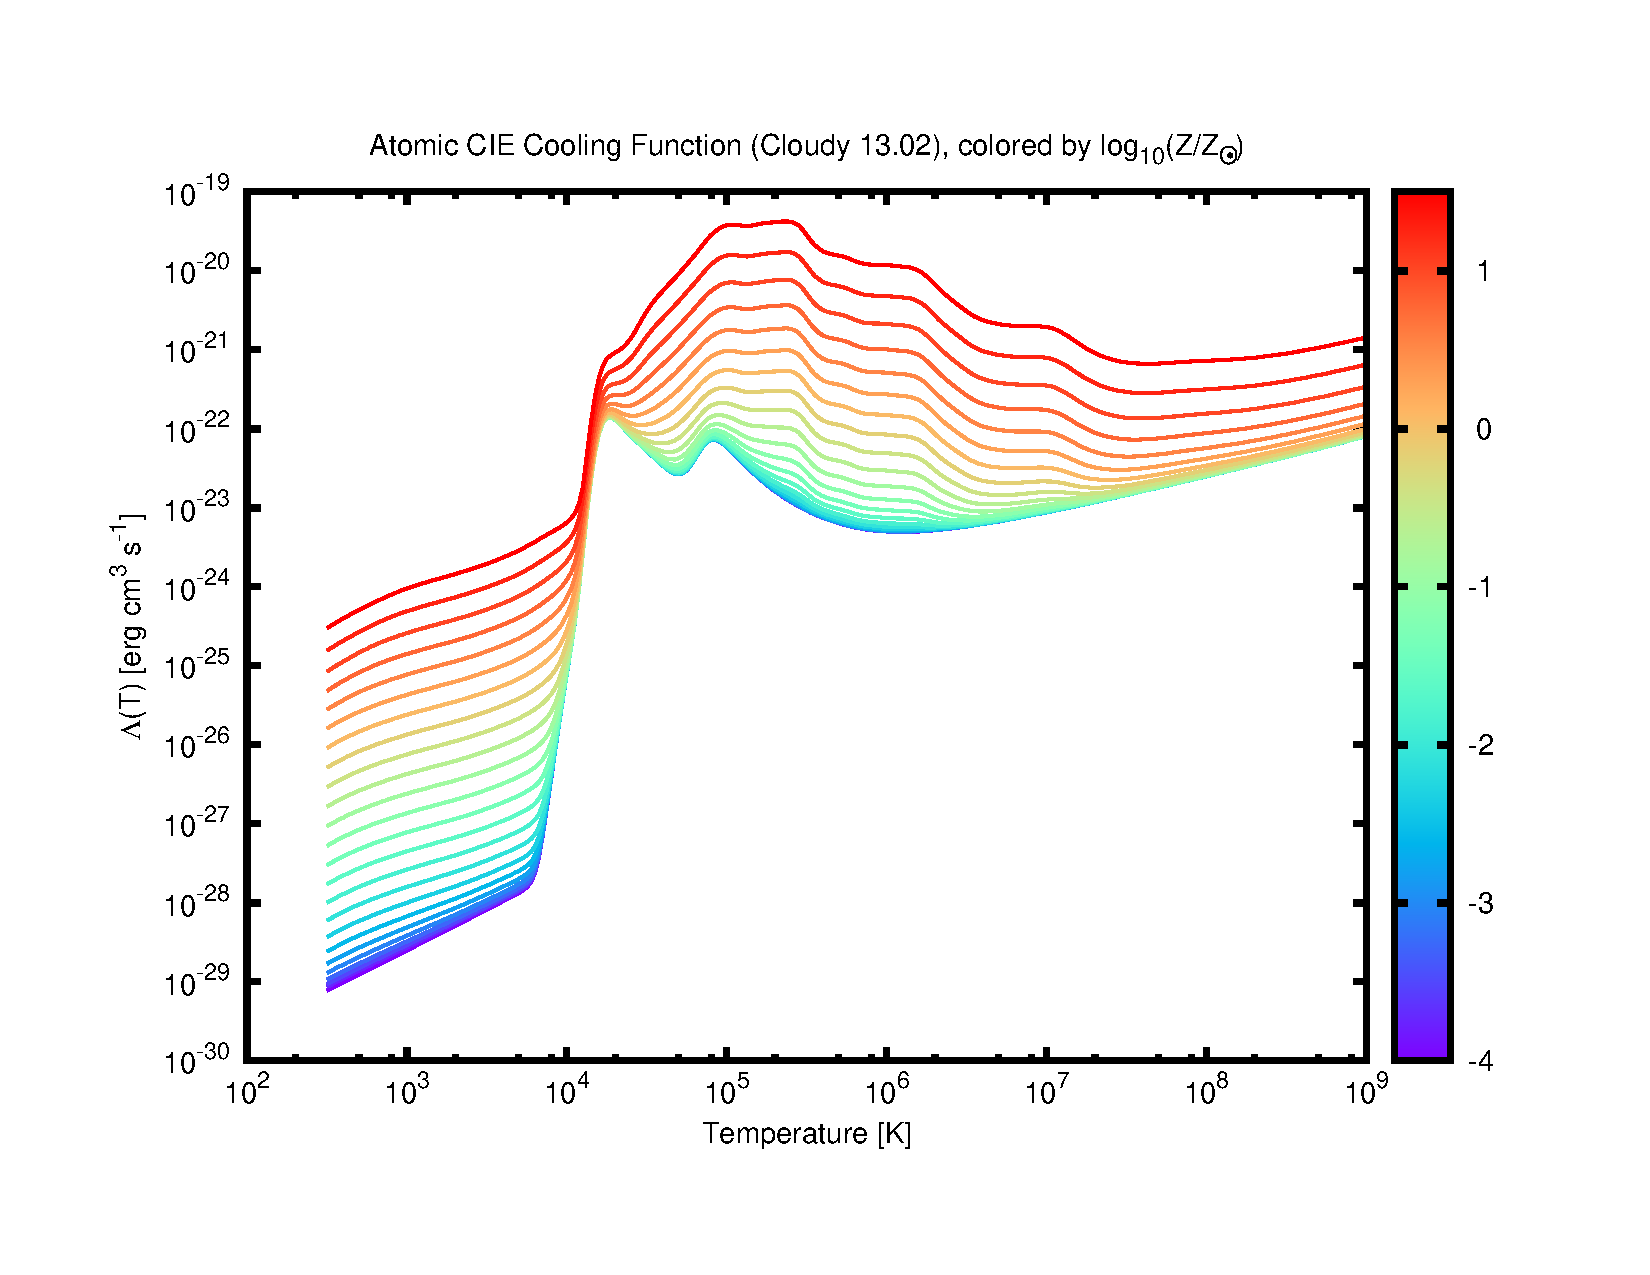
\includegraphics[width=160mm]{../plots/cooling_function_Atomic_CIE_Cloudy.pdf}
 \end{center}
 \caption{Cooling function for atomic gas in collisional ionization equilibrium computed using Cloudy 08.00.}
 \label{fig:atomicCIECloudyCoolingFunction}
\end{figure}

\subsubsection{Cooling Radius}

Additional methods for cooling radius calculations can be added using the {\tt coolingRadiusMethod} directive. The directive should contain a single argument, giving the name of a subroutine to be called to initialize the method. For example, the {\tt simple} method is described by a directive:
\begin{verbatim}
 !# <coolingRadiusMethod>
 !#  <unitName>Cooling_Radius_Simple_Initialize</unitName>
 !# </coolingRadiusMethod>
\end{verbatim}
Here, {\tt Cooling\_Radius\_Simple\_Initialize} is the name of a subroutine which will be called to initialize the method. The initialization subroutine must have the following form:
\begin{verbatim}
  subroutine Method_Initialize(coolingRadiusMethod,Cooling_Radius_Get,Cooling_Radius_Growth_Rate_Get)
    implicit none
    type(varying_string),          intent(in)    :: coolingRadiusMethod
    procedure(),          pointer, intent(inout) :: Cooling_Radius_Get,Cooling_Radius_Growth_Rate_Get
    
    if (coolingRadiusMethod == 'myMethod') then
       Cooling_Radius_Get => My_Method_Get_Procedure
       Cooling_Radius_Growth_Rate_Get => My_Method_Growth_Rate_Get_Procedure
    end if
    return
  end subroutine Method_Initialize
\end{verbatim}
where {\tt myMethod} is the name of this method as will be specified by the {\tt coolingRadiusMethod} input parameter. The procedure pointer {\tt Cooling\_Radius\_Get} must be set to point to a function which returns the cooling function as described below while {\tt Cooling\_Radius\_Growth\_Rate\_Get} should be set to point to a function which returns the rate at which the cooling radius is growing. The initialization subroutine should perform any other tasks required to initialize the module (such as reading parameters etc.).

The cooling radius function must have the form:
\begin{verbatim}
 double precision function Cooling_Radius_Get(thisNode)
    implicit none
    type(treeNode), intent(inout), pointer :: thisNode
    .
    .
    .
    return
 end function Cooling_Radius_Get
\end{verbatim}
The function must return the cooling radius (in units of Mpc) for {\tt thisNode}. The cooling radius growth rate function should have the same template but return the rate at which the cooling radius grows in units of Mpc/Gyr.

Currently defined cooling radius methods are:
\begin{description}
 \item [\hyperlink{cooling.cooling_radius.simple.F90:cooling_radii_simple:cooling_radius_simple}{{\tt simple}}] Computes the cooling radius by seeking the radius at which the time available for cooling equals the cooling time. The growth rate is determined consistently based on the slope of the density profile, the density dependence of the cooling function and the rate at which the time available for cooling is increasing. This method assumes that the cooling time is a monotinc function of radius.
\end{description}

\subsubsection{Cooling Rate}

Additional methods for the cooling rate from the hot halo can be added using the {\tt coolingRateMethod} directive. The directive should contain a single argument, giving the name of a subroutine to be called to initialize the method. For example, the {\tt White + Frenk} method is described by a directive:
\begin{verbatim}
 !# <coolingRateMethod>
 !#  <unitName>Cooling_Rate_White_Frenk_Initialize</unitName>
 !# </coolingRateMethod>
\end{verbatim}
Here, {\tt Cooling\_Rate\_White\_Frenk\_Initialize} is the name of a subroutine which will be called to initialize the method. The initialization subroutine must have the following form:
\begin{verbatim}
  subroutine Method_Initialize(coolingRateMethod,Cooling_Rate_Get)
    implicit none
    type(varying_string),          intent(in)    :: coolingRateMethod
    procedure(),          pointer, intent(inout) :: Cooling_Rate_Get
    
    if (coolingRateMethod == 'myMethod') Cooling_Rate_Get => My_Method_Get
    return
  end subroutine Method_Initialize
\end{verbatim}
where {\tt myMethod} is the name of this method as will be specified by the {\tt coolingRateMethod} input parameter. The procedure pointer {\tt Cooling\_Rate\_Get} must be set to point to a function which returns the cooling rate from the hot halo. The initialization subroutine should perform any other tasks required to initialize the module (such as reading parameters etc.).

The cooling rate function must have the form:
\begin{verbatim}
 double precision function Cooling_Rate_Get(thisNode)
    implicit none
    type(treeNode),   intent(inout), pointer :: thisNode
    .
    .
    .
    return
 end function Cooling_Rate_Get
\end{verbatim}
The function must return the rate of mass drop-out from the hot halo (in units of $M_\odot$/Gyr) for {\tt thisNode}. 

Currently defined cooling rate methods are:
\begin{description}
 \item [\hyperlink{cooling.cooling_rate.White-Frenk.F90:cooling_rates_white_frenk:cooling_rate_white_frenk}{{\tt White + Frenk}}] Implements something similar to that proposed by \cite{white_galaxy_1991}. Namely, the cooling rate is set equal to
 \begin{equation}
  \dot{M}_{\rm cool} = 4 \pi \rho(r_{\rm cool}) r_{\rm cool}^2 \dot{r}_{\rm cool}
 \end{equation}
 if the cooling radius is within the virial radius and
 \begin{equation}
  \dot{M}_{\rm cool} = {M_{\rm hot} \over \tau_{\rm dynamical,halo}}
 \end{equation}
 otherwise.
\end{description}

\subsubsection{Cooling Time}

Additional methods for cooling time calculations can be added using the {\tt coolingTimeMethod} directive. The directive should contain a single argument, giving the name of a subroutine to be called to initialize the method. For example, the {\tt simple} method is described by a directive:
\begin{verbatim}
 !# <coolingTimeMethod>
 !#  <unitName>Cooling_Time_Simple_Initialize</unitName>
 !# </coolingTimeMethod>
\end{verbatim}
Here, {\tt Cooling\_Time\_Simple\_Initialize} is the name of a subroutine which will be called to initialize the method. The initialization subroutine must have the following form:
\begin{verbatim}
  subroutine Method_Initialize(coolingTimeMethod,Cooling_Time_Get,Cooling_Time_Density_Log_Slope_Get,Cooling_Time_Temperature_Log_Slope_Get)
    implicit none
    type(varying_string),          intent(in)    :: coolingTimeMethod
    procedure(),          pointer, intent(inout) :: Cooling_Time_Get,Cooling_Time_Density_Log_Slope_Get,Cooling_Time_Temperature_Log_Slope_Get
    
    if (coolingTimeMethod == 'myMethod') then
       Cooling_Time_Get => My_Method_Get_Procedure
       Cooling_Time_Density_Log_Slope_Get => My_Method_Density_Log_Slope_Procedure
       Cooling_Time_Temperature_Log_Slope_Get => My_Method_Temperature_Log_Slope_Procedure
    end if
    return
  end subroutine Method_Initialize
\end{verbatim}
where {\tt myMethod} is the name of this method as will be specified by the {\tt coolingTimeMethod} input parameter. The procedure pointer {\tt Cooling\_Time\_Get} must be set to point to a function which returns the cooling function as described below while the other two pointers should point to functions which return the appropriate logarithmic slope. The initialization subroutine should perform any other tasks required to initialize the module (such as reading parameters etc.).

The cooling radius function must have the form:
\begin{verbatim}
 double precision function Cooling_Time_Get(temperature,density,abundances,radiation)
    implicit none
    double precision,          intent(in) :: temperature,density
    type(abundancesStructure), intent(in) :: abundances
    type(radiationStructure),  intent(in) :: radiation
    .
    .
    .
    return
 end function Cooling_Time_Get
\end{verbatim}
The function must return the cooling time (in units of Gyr) for at the specified {\tt temperature}, {\tt density} and for composition and radiation field as specified by the {\tt abundances} and {\tt radiation} structures. The logarithmic slope functions should have the same template, but return the logarithmic slope of the cooling time with respect to the appropriate variable instead.

Currently defined cooling time methods are:
\begin{description}
 \item [\hyperlink{cooling.cooling_time.simple.F90:cooling_times_simple:cooling_time_simple}{{\tt simple}}] Compute the cooling time as the ratio of the gas thermal energy density to the volume rate of radiative energy loss. The gas is assumed to have an effective number of degrees of freedom specified by the {\tt coolingTimeSimpleDegreesOfFreedom} parameter.
\end{description}

\subsubsection{Cosmology}

Additional methods for cosmology can be added using the {\tt cosmologyMethod} directive. The directive should contain a single argument, giving the name of a subroutine to be called to initialize the method. For example, the {\tt matter + lambda} method is described by a directive:
\begin{verbatim}
  !# <cosmologyMethod>
  !#  <unitName>Cosmology_Functions_Matter_Lambda_Initialize</unitName>
  !# </cosmologyMethod>
\end{verbatim}
Here, {\tt Cosmology\_Functions\_Matter\_Lambda\_Initialize} is the name of a subroutine which will be called to initialize the method. The initialization subroutine must have the following form:
\begin{verbatim}
  subroutine Method_Initialize(cosmologyMethod,Expansion_Factor_Is_Valid_Get,Cosmic_Time_Is_Valid_Get &
       &,Cosmology_Age_Get,Expansion_Factor_Get,Hubble_Parameter_Get,Early_Time_Density_Scaling_Get  & 
       &,Omega_Matter_Get,Omega_Dark_Energy_Get,Expansion_Rate_Get,Epoch_of_Matter_Dark_Energy_Equality_Get &
       &,Epoch_of_Matter_Domination_Get,Epoch_of_Matter_Curvature_Equality_Get,CMB_Temperature_Get)
    implicit none
    type(varying_string),          intent(in)    :: cosmologyMethod
    procedure(),          pointer, intent(inout) :: Expansion_Factor_Is_Valid_Get,Cosmic_Time_Is_Valid_Get &
       &,Cosmology_Age_Get,Expansion_Factor_Get,Hubble_Parameter_Get,Early_Time_Density_Scaling_Get  & 
       &,Omega_Matter_Get,Omega_Dark_Energy_Get,Expansion_Rate_Get,Epoch_of_Matter_Dark_Energy_Equality_Get &
       &,Epoch_of_Matter_Domination_Get,Epoch_of_Matter_Curvature_Equality_Get,CMB_Temperature_Get
    
    if (cosmologyMethod == 'myMethod') then
       Procedure_Pointer_Get => My_Procedure
       .
       .
       .
    end if
    return
  end subroutine Method_Initialize
\end{verbatim}
where {\tt myMethod} is the name of this method as will be specified by the {\tt cosmologyMethod} input parameter. Numerous procedure pointers are passed in and should be set to point to functions/subroutines that perform cosmological calcalculations as described below. The initialization subroutine should perform any other tasks required to initialize the module (such as reading parameters etc.).

Below are a list of procedure templates for the various procedures required by the cosmology method. After each template a description of what the procedure must do is given.

\begin{verbatim}
   logical function My_Expansion_Factor_Is_Valid(aExpansion)
     implicit none
     double precision, intent(in) :: aExpansion
     .
     .
     .
     return
   end function My_Expansion_Factor_Is_Valid
\end{verbatim}
Should return true if the input expansion factor is valid (e.g. greater than zero and less the the maximum expansion factor for a collapsing universe).

\begin{verbatim}
   logical function My_Cosmic_Time_Is_Valid(time)
     implicit none
     double precision, intent(in) :: time
     .
     .
     .
     return
   end function My_Cosmic_Time_Is_Valid
\end{verbatim}
Should return true if the input cosmic time is valid (e.g. greater than zero and less than the time at the Big Crunch in collapsing universes).

\begin{verbatim}
   double precision function My_Cosmology_Age(aExpansion,collapsingPhase)
     implicit none
     double precision, intent(in)           :: aExpansion
     logical,          intent(in), optional :: collapsingPhase
     .
     .
     .
     return
   end function My_Cosmology_Age
\end{verbatim}
Should return the age (in Gyr) of the universe at a given expansion factor. The {\tt collapsingPhase} argument optionally specififies whether the age during the expanding or collapsing phase is required---if absent then the expanding phase should be assumed.

\begin{verbatim}
   double precision function My_Expansion_Factor(tCosmological)
     implicit none
     double precision, intent(in) :: tCosmological
     .
     .
     .
     return
   end function My_Expansion_Factor
\end{verbatim}
Should return the expansion factor of the universe at the input cosmological time (given in Gyr).

\begin{verbatim}
   double precision function My_Expansion_Rate(aExpansion)
     implicit none
     double precision, intent(in) :: aExpansion
     .
     .
     .
     return
   end function My_Expansion_Rate
\end{verbatim}
Should return the expansion rate, $\dot{a}/a$ (in Gyr$^{-1}$), at the given expansion factor.

\begin{verbatim}
   double precision function My_Hubble_Parameter(tCosmological,aExpansion,collapsingPhase)
     implicit none
     double precision, intent(in), optional :: tCosmological,aExpansion
     logical,          intent(in), optional :: collapsingPhase
     .
     .
     .
     return
   end function My_Hubble_Parameter
\end{verbatim}
Should return the Hubble parameter (in km/s/Mpc) at the given cosmic epoch. The cosmic epoch can be specified as a time since the Big Bang, or an expansion factor (in the expanding phase unless the collapsing phase is specifically requested). Specifying a time and an expansion factor is invalid input, and the routine should abort in such cases.

\begin{verbatim}
   subroutine My_Early_Time_Density_Scaling(dominateFactor,densityPower,aDominant,Omega_Dominant)
     implicit none
     double precision, intent(in)            :: dominateFactor
     double precision, intent(out)           :: densityPower,aDominant
     double precision, intent(out), optional :: Omega_Dominant
     .
     .
     .
     return
   end subroutine My_Early_Time_Density_Scaling
\end{verbatim}
Should compute the epoch, {\tt aDominant}, before which the universe is dominated by a single component (e.g. in a matter and cosmological constant only universe, the epoch before which matter always dominated). The epoch should be such that the component in question dominates over others in density by a factor of {\tt dominateFactor}. The exponent in the density-expansion factor relation for this relation should be returned in {\tt densityPower}. If present, {\tt Omega\_Dominant} should be set to the density of the dominant component (in units of the critical density) at the present day.

\begin{verbatim}
   double precision function My_Epoch_of_Matter_Domination(dominateFactor)
     implicit none
     double precision, intent(in) :: dominateFactor
      .
     .
     .
    return
   end function My_Epoch_of_Matter_Domination
\end{verbatim}
Should return the epoch at which matte dominates the energy density of the universe by the specified factor.

\begin{verbatim}
   double precision function My_Omega_Matter(tCosmological,aExpansion,collapsingPhase)
     implicit none
     double precision, intent(in), optional :: tCosmological,aExpansion
     logical,          intent(in), optional :: collapsingPhase
     .
     .
     .
     return
   end function My_Omega_Matter
\end{verbatim}
Should return $\Omega_{\rm M}$ at the given cosmic epoch. The cosmic epoch can be specified as a time since the Big Bang, or an expansion factor (in the expanding phase unless the collapsing phase is specifically requested). Specifying a time and an expansion factor is invalid input, and the routine should abort in such cases.

\begin{verbatim}
   double precision function My_Omega_Dark_Energy(tCosmological,aExpansion,collapsingPhase)
     implicit none
     double precision, intent(in), optional :: tCosmological,aExpansion
     logical,          intent(in), optional :: collapsingPhase
     .
     .
     .
     return
   end function My_Omega_Dark_Energy
\end{verbatim}
Should return $\Omega_\Lambda$ at the given cosmic epoch. The cosmic epoch can be specified as a time since the Big Bang, or an expansion factor (in the expanding phase unless the collapsing phase is specifically requested). Specifying a time and an expansion factor is invalid input, and the routine should abort in such cases.

\begin{verbatim}
   double precision function My_Epoch_of_Matter_Dark_Energy_Equality(requestType)
     implicit none
     integer, intent(in) :: requestType
     .
     .
     .
     return
   end function My_Epoch_of_Matter_Dark_Energy_Equality
\end{verbatim}
Should return the cosmic epoch at which matter and dark energy have equal energy densities. If {\tt requestType} is {\tt requestTypeTime} (specified in the {\tt Cosmology\_Functions\_Parameters} module) then cosmic time (in Gyr) should be returned, while if it is {\tt requestTypeExpansionFactor} then expansion factor should be returned instead.

\begin{verbatim}
   double precision function My_Epoch_of_Matter_Curvature_Equality(requestType)
     implicit none
     integer, intent(in) :: requestType
     .
     .
     .
     return
   end function My_Epoch_of_Matter_Curvature_Equality
\end{verbatim}
Should return the cosmic epoch at which matter and curvature have equal energy densities. If {\tt requestType} is {\tt requestTypeTime} (specified in the {\tt Cosmology\_Functions\_Parameters} module) then cosmic time (in Gyr) should be returned, while if it is {\tt requestTypeExpansionFactor} then expansion factor should be returned instead.

\begin{verbatim}
   double precision function My_CMB_Temperature(tCosmological,aExpansion,collapsingPhase)
     implicit none
     double precision, intent(in), optional :: tCosmological,aExpansion
     logical,          intent(in), optional :: collapsingPhase
     .
     .
     .
     return
   end function My_CMB_Temperature
\end{verbatim}
Should return the \CMB\ temperature (in K) at the given cosmic epoch. The cosmic epoch can be specified as a time since the Big Bang, or an expansion factor (in the expanding phase unless the collapsing phase is specifically requested). Specifying a time and an expansion factor is invalid input, and the routine should abort in such cases.

Currently defined cosmology methods are:
\begin{description}
 \item [{\tt matter + lambda}] Cosmological relations are computed assuming a universe that contains only matter and a cosmological constant.
\end{description}

\subsubsection{Critical Overdensity for Halo Collapse}

Additional methods for the critical linear theory overdensity for halo collapse can be added using the {\tt criticalOverdensityMethod} directive. The directive should contain a single argument, giving the name of a subroutine to be called to initialize the method. For example, the {\tt spherical top hat} method is described by a directive:
\begin{verbatim}
  !# <criticalOverdensityMethod>
  !#  <unitName>Spherical_Collape_Delta_Critical_Initialize</unitName>
  !# </criticalOverdensityMethod>
\end{verbatim}
Here, {\tt Spherical\_Collape\_Delta\_Critical\_Initialize} is the name of a subroutine which will be called to initialize the method. The initialization subroutine must have the following form:
\begin{verbatim}
  subroutine Method_Initialize(criticalOverdensityMethod,Critical_Overdensity_Tabulate)
    implicit none
    type(varying_string),          intent(in)    :: criticalOverdensityMethod
    procedure(),          pointer, intent(inout) :: Critical_Overdensity_Tabulate
    
    if (criticalOverdensityMethod.eq.'myMethod') then
       Critical_Overdensity_Tabulate => My_Do_Tabulate
       .
       .
       .
    end if
    return
  end subroutine Method_Initialize
\end{verbatim}
where {\tt myMethod} is the name of this method as will be specified by the {\tt criticalOverdensityMethod} input parameter. The procedure pointer {\tt Critical\_Overdensity\_Tabulate} must be set to point to a subroutine which tabulates the critical overdensity as described below. The initialization subroutine should perform any other tasks required to initialize the module (such as reading parameters etc.).

The tabulation subroutine must have the form:
\begin{verbatim}
   subroutine Critical_Overdensity_Tabulate(time,deltaCritNumberPoints,deltaCritTime,deltaCritDeltaCrit)
    implicit none
    double precision, intent(in)                               :: time
    integer,          intent(out)                              :: deltaCritNumberPoints
    double precision, intent(inout), allocatable, dimension(:) :: deltaCritTime,deltaCritDeltaVirial
    .
    .
    .
    return
   end subroutine Critical_Overdensity_Tabulate
\end{verbatim}
The subroutine must tabulate the critical overdensity in array {\tt deltaCritDeltaVirial()} as a function of wavenumber {\tt deltaCritTime()} (these arrays must be allocated to the correct size, and may be prevously allocated, therefore requiring a deallocation). The number of tabulated points should be returned in {\tt deltaCritNumberPoints}. The subroutine should ensure that the currently requested {\tt time} is within the range of the tabulated function (preferably with some buffer).

Currently defined critical overdensity methods are:
\begin{description}
 \item [{\tt spherical top hat}] The critical overdensity is computed for a Universe containing collisionless matter and a cosmological constant following the spherical top hat collapse model (see, for example, \citealt{percival_cosmological_2005}).
\end{description}

\subsubsection{Dark Matter Density Profile Concentration}

Additional methods for the dark matter density profile concentration can be added using the {\tt darkMatterConcentrationMethod} directive. The directive should contain a single argument, giving the name of a subroutine to be called to initialize the method. For example, the {\tt Gao2008} method is described by a directive:
\begin{verbatim}
 !# <darkMatterConcentrationMethod>
 !#  <unitName>Dark_Matter_Concentrations_Gao20008_Initialize</unitName>
 !# </darkMatterConcentrationMethod>
\end{verbatim}
Here, {\tt Dark\_Matter\_Concentrations\_Gao20008\_Initialize} is the name of a subroutine which will be called to initialize the method. The initialization subroutine must have the following form:
\begin{verbatim}
  subroutine Method_Initialize(darkMatterConcentrationMethod,Dark_Matter_Profile_Concentration_Get)
    implicit none
    type(varying_string),          intent(in)    :: darkMatterConcentrationMethod
    procedure(),          pointer, intent(inout) :: Dark_Matter_Profile_Concentration_Get
    
    if (darkMatterConcentrationMethod == 'myMethod') then
       Dark_Matter_Profile_Concentration_Get => My_Concentration_Get
       .
       .
       .
    end if
    return
  end subroutine Method_Initialize
\end{verbatim}
where {\tt myMethod} is the name of this method as will be specified by the {\tt criticalOverdensityMethod} input parameter. The procedure pointer {\tt Dark\_Matter\_Profile\_Concentration\_Get} must be set to point to a function which returns the concentration of a node. The initialization subroutine should perform any other tasks required to initialize the module (such as reading parameters etc.).

The concentration function must have the form:
\begin{verbatim}
  double precision function My_Dark_Matter_Profile_Concentration(thisNode)
    implicit none
    type(treeNode), intent(inout), pointer :: thisNode
    .
    .
    .
    return
  end function My_Dark_Matter_Profile_Concentration
\end{verbatim}
The function should compute and return the concentration for {\tt thisNode}.

Currently defined critical overdensity methods are:
\begin{description}
 \item [{\tt Gao2008}] The concentration is computed using a fitting function from \cite{gao_redshift_2008}.
\end{description}

\subsubsection{Bar Instabilities}

Additional methods for bar instabilities in disks can be added using the {\tt barInstabilityMethod} directive. The directive should contain a single argument, giving the name of a subroutine to be called to initialize the method. For example, the {\tt ELN} method is described by a directive:
\begin{verbatim}
 !# <barInstabilityMethod>
 !#  <unitName>Galactic_Dynamics_Bar_Instabilities_ELN_Initialize</unitName>
 !# </barInstabilityMethod>
\end{verbatim}
Here, {\tt Galactic\_Dynamics\_Bar\_Instabilities\_ELN\_Initialize} is the name of a subroutine which will be called to initialize the method. The initialization subroutine must have the following form:
\begin{verbatim}
  subroutine Method_Initialize(barInstabilityMethod,Bar_Instability_Timescale_Get)
    implicit none
    type(varying_string),          intent(in)    :: barInstabilityMethod
    procedure(),          pointer, intent(inout) :: Bar_Instability_Timescale_Get
    
    if (barInstabilityMethod == 'myMethod') then
       Bar_Instability_Timescale_Get => My_Bar_Instability_Timescale_Get
       .
       .
       .
    end if
    return
  end subroutine Method_Initialize
\end{verbatim}
where {\tt myMethod} is the name of this method as will be specified by the {\tt barInstabilityMethod} input parameter. The procedure pointer {\tt Bar\_Instability\_Timescale\_Get} must be set to point to a function which returns the timescale on which the bar instability depletes material from the disk to the pseudo-bulge. The initialization subroutine should perform any other tasks required to initialize the module (such as reading parameters etc.).

The bar instability timesacale function must have the form:
\begin{verbatim}
  double precision function My_Bar_Instability_Timescale(thisNode)
    implicit none
    type(treeNode), intent(inout), pointer :: thisNode
    .
    .
    .
    return
  end function My_Bar_Instability_Timescale
\end{verbatim}
The function should compute and return the timescale (in Gyr) for the bar instability in the disk in {\tt thisNode} to transfer material from the disk to the pseudo-bulge. If no instability is present, a negative timescale should be returned.

Currently defined bar instability methods are:
\begin{description}
 \item [{\tt null}] A null method in which disks are never bar unstable;
 \item [{\tt ELN}] The bar instability is determined using the algorithm of \cite{efstathiou_stability_1982}.
\end{description}

\subsubsection{Galactic Component Radii Solver}\label{sec:galactic_radii_solvers}

Additional methods for solving for radii of galactic components can be added using the {\tt galacticStructureRadiusSolverMethod} directive. The directive should contain a single argument, giving the name of a subroutine to be called to initialize the method. For example, the {\tt simple} method is described by a directive:
\begin{verbatim}
 !# <galacticStructureRadiusSolverMethod>
 !#  <unitName>Galactic_Structure_Radii_Simple_Initialize</unitName>
 !# </galacticStructureRadiusSolverMethod>
\end{verbatim}
Here, {\tt Galactic\_Structure\_Radii\_Simple\_Initialize} is the name of a subroutine which will be called to initialize the method. The initialization subroutine must have the following form:
\begin{verbatim}
  subroutine Method_Initialize(galacticStructureRadiusSolverMethod,Galactic_Structure_Radii_Solve_Do)
    implicit none
    type(varying_string),          intent(in)    :: galacticStructureRadiusSolverMethod
    procedure(),          pointer, intent(inout) :: Galactic_Structure_Radii_Solve_Do
    
    if (galacticStructureRadiusSolverMethod == 'myMethod') Galactic_Structure_Radii_Solve_Do => My_Method_Do_Procedure
    return
  end subroutine Method_Initialize
\end{verbatim}
where {\tt myMethod} is the name of this method as will be specified by the {\tt galacticStructureRadiusSolverMethod} input parameter. The procedure pointer {\tt Galactic\_Structure\_Radii\_Solve\_Do} must be set to point to a subroutine which solves for the radii of components in a node as described below. The initialization subroutine should perform any other tasks required to initialize the module (such as reading parameters etc.).

The radii solving subroutine must have the form:
\begin{verbatim}
 subroutine Radii_Solver_Do(thisNode)
    implicit none
    type(treeNode), intent(in), pointer :: thisNode
    .
    .
    .
    return
 end subroutine Radii_Solver_Do
\end{verbatim}
The function must set the radii (and corresponding circular velocities) of all components that have a radius property in {\tt thisNode}.

Currently defined radius solver methods are:
\begin{description}
 \item [\hyperlink{galactic_structure.radius_solver.simple.F90:galactic_structure_radii_simple:galactic_structure_radii_solve_simple}{{\tt simple}}] This solver computes radii assuming that the gravitational potential is dominated by dark matter (i.e. no baryonic self-gravity is included) and that dark matter does not respond to the presence of baryons (i.e. no adiabatic contraction). It uses the ``radius solver'' (see \S\ref{sec:radius_solver}) task to interact with the node.
 \item [\hyperlink{galactic_structure.radius_solver.adiabatic.F90:galactic_structure_radii_adiabatic:galactic_structure_radii_solve_adiabatic}{{\tt adiabatic}}] This solver computes radii including the effects of self-gravity of the baryonic component and adiabatic contraction of the dark matter halo using the method of \cite{gnedin_response_2004}. It uses the ``radius solver'' (see \S\ref{sec:radius_solver}) task to interact with the node.
\end{description}

\subsubsection{Hot Halo Density Profile}

Additional methods for the hot halo density profile can be added using the {\tt hotHaloDensityMethod} directive. The directive should contain a single argument, giving the name of a subroutine to be called to initialize the method. For example, the {\tt cored isothermal} method is described by a directive:
\begin{verbatim}
 !# <hotHaloDensityMethod>
 !#  <unitName>Hot_Halo_Density_Cored_Isothermal</unitName>
 !# </hotHaloDensityMethod>
\end{verbatim}
Here, {\tt Hot\_Halo\_Density\_Cored\_Isothermal} is the name of a subroutine which will be called to initialize the method. The initialization subroutine must have the following form:
\begin{verbatim}
  subroutine Method_Initialize(hotHaloDensityMethod,Hot_Halo_Density_Get,Hot_Halo_Density_Log_Slope_Get)
    implicit none
    type(varying_string),          intent(in)    :: hotHaloDensityMethod
    procedure(),          pointer, intent(inout) :: Hot_Halo_Density_Get,Hot_Halo_Density_Log_Slope_Get
    
    if (hotHaloDensityMethod == 'myMethod') then
       Hot_Halo_Density_Get => My_Method_Get
       Hot_Halo_Density_Log_Slope_Get => My_Method_Log_Slope_Get
    end if
    return
  end subroutine Method_Initialize
\end{verbatim}
where {\tt myMethod} is the name of this method as will be specified by the {\tt hotHaloDensityMethod} input parameter. The procedure pointer {\tt Hot\_Halo\_Density\_Get} must be set to point to a function which returns the hot halo density as described below while {\tt Hot\_Halo\_Density\_Log\_Slope\_Get} should be set to point to a function which returns the logarithmic slope of that profile. The initialization subroutine should perform any other tasks required to initialize the module (such as reading parameters etc.).

The density function must have the form:
\begin{verbatim}
 double precision function Hot_Halo_Density_Get(thisNode,radius)
    implicit none
    type(treeNode),   intent(inout), pointer :: thisNode
    double precision, intent(in)             :: radius
    .
    .
    .
    return
 end function Hot_Halo_Density_Get
\end{verbatim}
The function must return the density (in units of $M_\odot$Mpc$^{-3}$) of the hot halo at the specified radius (given in Mpc) for {\tt thisNode}. The logarithmic slope function should have the same template but return the logarithmic slope of the density profile at the specified radius.

Currently defined hot halo density profile methods are:
\begin{description}
 \item [\hyperlink{hot_halo.density_profile.cored_isothermal.F90:hot_halo_density_profile_cored_isothermal:hot_halo_density_cored_isothermal_get}{{\tt cored isothermal}}] Implements a cored isothermal profile for the hot halo. The density is given by
 \begin{equation}
  \rho(r) = {\rho_0 \over 1 + (r/r_{\rm core})^2}
 \end{equation}
 where the normalization is chosen to ensure the correct hot halo mass within the virial radius, and $r_{\rm core}=${\tt isothermalCoreRadiusOverVirialRadius}$r_{\rm virial}$ where {\tt isothermalCoreRadiusOverVirialRadius} is an input parameter.
\end{description}

\subsubsection{Hot Halo Temperature Profile}

Additional methods for the hot halo temperature profile can be added using the {\tt hotHaloTemperatureMethod} directive. The directive should contain a single argument, giving the name of a subroutine to be called to initialize the method. For example, the {\tt virial} method is described by a directive:
\begin{verbatim}
 !# <hotHaloTemperatureMethod>
 !#  <unitName>Hot_Halo_Temperature_Virial</unitName>
 !# </hotHaloTemperatureMethod>
\end{verbatim}
Here, {\tt Hot\_Halo\_Temperature\_Virial} is the name of a subroutine which will be called to initialize the method. The initialization subroutine must have the following form:
\begin{verbatim}
  subroutine Method_Initialize(hotHaloTemperatureMethod,Hot_Halo_Temperature_Get,Hot_Halo_Temperature_Logarithmic_Slope_Get)
    implicit none
    type(varying_string),          intent(in)    :: hotHaloTemperatureMethod
    procedure(),          pointer, intent(inout) :: Hot_Halo_Temperature_Get,Hot_Halo_Temperature_Logarithmic_Slope_Get
    
    if (hotHaloTemperatureMethod == 'myMethod') then
       Hot_Halo_Temperature_Get => My_Method_Get
       Hot_Halo_Temperature_Logarithmic_Slope_Get => My_Method_Logarithmic_Slope_Get
    end if
    return
  end subroutine Method_Initialize
\end{verbatim}
where {\tt myMethod} is the name of this method as will be specified by the {\tt hotHaloTemperatureMethod} input parameter. The procedure pointer {\tt Hot\_Halo\_Temperature\_Get} must be set to point to a function which returns the hot halo density as described below while {\tt Hot\_Halo\_Temperature\_Logarithmic\_Slope\_Get} must point to a function which returns the logarithmic slope of the temperature profile. The initialization subroutine should perform any other tasks required to initialize the module (such as reading parameters etc.).

The temperature function must have the form:
\begin{verbatim}
 double precision function Hot_Halo_Temperature_Get(thisNode,radius)
    implicit none
    type(treeNode),   intent(inout), pointer :: thisNode
    double precision, intent(in)             :: radius
    .
    .
    .
    return
 end function Hot_Halo_Temperature_Get
\end{verbatim}
The function must return the temperature (in Kelvin) of the hot halo at the specified radius (given in Mpc) for {\tt thisNode}. The logarithmic slope function should have the same template, but return $\d\ln T / \d \ln r$.

Currently defined hot halo density profile methods are:
\begin{description}
 \item [\hyperlink{hot_halo.temperature_profile.virial.F90:hot_halo_temperature_profile_virial:hot_halo_temperature_virial_get}{{\tt virial}}] Implements an isothermal profile with temperature equal to the virial temperature.
\end{description}

\subsubsection{Halo Mass Functions}

Additional methods for the halo mass function can be added using the {\tt haloMassFunctionMethod} directive. The directive should contain a single argument, giving the name of a subroutine to be called to initialize the method. For example, the {\tt Press-Schechter} method is described by a directive:
\begin{verbatim}
 !# <haloMassFunctionMethod>
 !#  <unitName>Halo_Mass_Function_Press_Schechter_Initialize</unitName>
 !# </haloMassFunctionMethod>
\end{verbatim}
Here, {\tt Halo\_Mass\_Function\_Press\_Schechter\_Initialize} is the name of a subroutine which will be called to initialize the method. The initialization subroutine must have the following form:
\begin{verbatim}
  subroutine Method_Initialize(haloMassFunctionMethod,Halo_Mass_Function_Tabulate)
    implicit none
    type(varying_string),          intent(in)    :: haloMassFunctionMethod
    procedure(),          pointer, intent(inout) :: Halo_Mass_Function_Tabulate
    
    if (haloMassFunctionMethod == 'myMethod') Halo_Mass_Function_Tabulate => My_Method_Tabulate
    return
  end subroutine Method_Initialize
\end{verbatim}
where {\tt myMethod} is the name of this method as will be specified by the {\tt haloMassFunctionMethod} input parameter. The procedure pointer {\tt Halo\_Mass\_Function\_Tabulate} must be set to point to a subrouine which returns a tabulation of the halo mass function. The initialization subroutine should perform any other tasks required to initialize the module (such as reading parameters etc.).

The halo mass function tabulating subroutine must have the form:
\begin{verbatim}
 double precision function Halo_Mass_Function_Tabulate(time,logMass,haloMassFunctionNumberPoints,haloMassFunctionLog
Mass,haloMassFunctionLogAbundance)
    implicit none
    double precision,                            intent(in)    :: time,logMass
    double precision, allocatable, dimension(:), intent(inout) :: haloMassFunctionLogMass,haloMassFunctionLogAbundance
    integer,                                     intent(out)   :: haloMassFunctionNumberPoints
    .
    .
    .
    return
 end function Halo_Spin_Sample_Get
\end{verbatim}
The subroutine should create a tabulation of the halo mass function for time {\tt time}, $\d n/\d M$ (in units of Mpc$^{-3} M_\odot^-1$) in the arrays {\tt haloMassFunctionLogMass} and {\tt haloMassFunctionLogAbundance}. These should be allocated to whatever size the method deems appropriate (they may need to be deallocated first) and the number of tabulated points returned in {\tt haloMassFunctionNumberPoints}. The subroutine should ensure that {\tt logMass} is included in the range of the tabulation.

Currently defined halo mass function methods are:
\begin{description}
 \item [\hyperlink{structure_formation.CDM.halo_mass_function.Press-Schechter.F90:halo_mass_function_press_schechter:halo_mass_function_press_schechter_tabulate}{{\tt Press-Schechter}}] Implements the Press-Schechter \citep{press_formation_1974} mass function.
 \item [\hyperlink{structure_formation.CDM.halo_mass_function.Sheth-Tormen.F90:halo_mass_function_sheth_tormen:halo_mass_function_sheth_tormen_tabulate}{{\tt Sheth-Tormen}}] Implements the Sheth-Tormen \citep{sheth_ellipsoidal_2001} mass function.
 \item [\hyperlink{structure_formation.CDM.halo_mass_function.Tinker2008.F90:halo_mass_function_tinker2008:halo_mass_function_tinker2008_tabulate}{{\tt Tinker2008}}] Implements the mass function described by \cite{tinker_towardhalo_2008}.
\end{description}

\subsubsection{Halo Spin Distribution}

Additional methods for the halo spin distribution can be added using the {\tt haloSpinDistributionMethod} directive. The directive should contain a single argument, giving the name of a subroutine to be called to initialize the method. For example, the {\tt lognormal} method is described by a directive:
\begin{verbatim}
 !# <haloSpinDistributionMethod>
 !#  <unitName>Halo_Spin_Distribution_Lognormal_Initialize</unitName>
 !# </haloSpinDistributionMethod>
\end{verbatim}
Here, {\tt Halo\_Spin\_Distribution\_Lognormal\_Initialize} is the name of a subroutine which will be called to initialize the method. The initialization subroutine must have the following form:
\begin{verbatim}
  subroutine Method_Initialize(haloSpinDistributionMethod,Halo_Spin_Sample_Get)
    implicit none
    type(varying_string),          intent(in)    :: haloSpinDistributionMethod
    procedure(),          pointer, intent(inout) :: Halo_Spin_Sample_Get
    
    if (haloSpinDistributionMethod == 'myMethod') Halo_Spin_Sample_Get => My_Method_Get
    return
  end subroutine Method_Initialize
\end{verbatim}
where {\tt myMethod} is the name of this method as will be specified by the {\tt haloSpinDistributionMethod} input parameter. The procedure pointer {\tt Halo\_Spin\_Sample\_Get} must be set to point to a function which returns a halo spin drawn at random from the distribution. The initialization subroutine should perform any other tasks required to initialize the module (such as reading parameters etc.).

The halo spin sampling function must have the form:
\begin{verbatim}
 double precision function Halo_Spin_Sample_Get(thisNode)
    implicit none
    type(treeNode),   intent(inout), pointer :: thisNode
    .
    .
    .
    return
 end function Halo_Spin_Sample_Get
\end{verbatim}
The function must return a halo spin drawn at random for the distribution appropriate to {\tt thisNode}. 

Currently defined halo spin distribution methods are:
\begin{description}
 \item [\hyperlink{dark_matter_halos.spins.distributions.lognormal.F90:halo_spin_distributions_lognormal:halo_spin_distribution_lognormal}{{\tt lognormal}}] Implements a lognormal distribution with median {\tt lognormalSpinDistributionMedian} and dispersion in $\ln\lambda$ of {\tt lognormalSpinDistributionSigma}, both of which are input parameters to \glc.
 \item [\hyperlink{dark_matter_halos.spins.distributions.Bett2007.F90:halo_spin_distributions_bett2007}{{\tt Bett2007}}] Implements distribution from \cite{bett_spin_2007} with parameter $\lambda_0=${\tt [spinDistributionBett2007Lambda0]} and $\alpha=${\tt [spinDistributionBett2007Alpha]}, both of which are input parameters to \glc.
\end{description}

\subsubsection{Halo Profiles}

Additional methods for the halo profile can be added using the {\tt haloProfileMethod} directive. The directive should contain a single argument, giving the name of a subroutine to be called to initialize the method. For example, the {\tt isothermal} method is described by a directive:
\begin{verbatim}
 !# <haloProfileMethod>
 !#  <unitName>Dark_Matter_Profile_Isothermal_Initialize</unitName>
 !# </haloProfileMethod>
\end{verbatim}
Here, {\tt Dark\_Matter\_Profile\_Isothermal\_Initialize} is the name of a subroutine which will be called to initialize the method. The initialization subroutine must have the following form:
\begin{verbatim}
  subroutine Method_Initialize(darkMatterProfileMethod,Dark_Matter_Profile_Energy_Get,Dark_Matter_Profile_Energy_Growth_Rate_Get,Dark_Matter_Profile_Rotation_Normalization_Get,Dark_Matter_Profile_Radius_from_Specific_Angular_Momentum_Get,Dark_Matter_Profile_Circular_Velocity_Get,Dark_Matter_Profile_Potential_Get,Dark_Matter_Profile_Enclosed_Mass_Get)
    implicit none
    type(varying_string),          intent(in)    :: darkMatterProfileMethod
    procedure(),          pointer, intent(inout) :: Dark_Matter_Profile_Energy_Get,Dark_Matter_Profile_Energy_Growth_Rate_Get,Dark_Matter_Profile_Rotation_Normalization_Get,Dark_Matter_Profile_Radius_from_Specific_Angular_Momentum_Get,Dark_Matter_Profile_Circular_Velocity_Get,Dark_Matter_Profile_Potential_Get,Dark_Matter_Profile_Enclosed_Mass_Get
    
    if (darkMatterProfileMethod == 'myMethod') then
       Dark_Matter_Profile_Energy_Get                                => My_Energy_Procedure
       Dark_Matter_Profile_Energy_Growth_Rate_Get                    => My_Energy_Growth_Rate_Procedure
       Dark_Matter_Profile_Rotation_Normalization_Get                => My_Rotation_Normalization_Procedure
       Dark_Matter_Profile_Radius_from_Specific_Angular_Momentum_Get => My_Radius_from_Specific_Angular_Momentum_Procedure
       Dark_Matter_Profile_Circular_Velocity_Get                     => My_Circular_Velocity_Procedure
       Dark_Matter_Profile_Potential_Get                             => My_Potential_Procedure
       Dark_Matter_Profile_Enclosed_Mass_Get                         => My_Enclosed_Mass_Procedure
    end if
    return
  end subroutine Method_Initialize
\end{verbatim}
where {\tt myMethod} is the name of this method as will be specified by the {\tt haloProfileMethod} input parameter. The procedure pointer {\tt Dark\_Matter\_Profile\_Energy\_Get} must be set to point to a function which returns the energy of the halo in units of $M_\odot$ km$^2$ s$^{-1}$ while {\tt Dark\_Matter\_Profile\_Energy\_Growth\_Rate\_Get} must point to a function which returns the rate of change of that energy. The {\tt Dark\_Matter\_Profile\_Rotation\_Normalization\_Get} should point to a function which provides the normalization of the rotation velocity vs. specific angular momentum relation for the halo such that, when multiplied by $4 \pi r^2 \d r \rho(r) V_{\rm rot}$ it gives the angular momentum of material between $r$ and $r+\d r$, i.e. it should return $A$ such that:
\begin{equation}
 J = A \langle j \rangle \int_0^{r_{\rm vir}} 4 \pi r^2 \d r \rho(r) r,
\end{equation}
where we ignore any variation of angular momentum within angle in each spherical shell of matter (since it will cancel out in later calculations anyway). {\tt Dark\_Matter\_Profile\_Radius\_from\_Specific\_Angular\_Momentum\_Get} must be set to point to a procedure which returns the radius in the halo at which circular orbits have the specified specific angular momentum. {\tt Dark\_Matter\_Profile\_Circular\_Velocity\_Get} must be set to point to a procedure which returns the circular velocity in the halo at a given radius.  {\tt Dark\_Matter\_Profile\_Potential\_Get} must be set to point to a procedure which returns the gravitational potential in the halo at a given radius.  {\tt Dark\_Matter\_Profile\_Enclosed\_Mass\_Get} must be set to point to a procedure which returns the mass enclosed in the halo at a given radius. The initialization subroutine should perform any other tasks required to initialize the module (such as reading parameters etc.).

The halo energy function must have the form:
\begin{verbatim}
 double precision function Dark_Matter_Profile_Energy_Get(thisNode)
    implicit none
    type(treeNode),   intent(inout), pointer :: thisNode
    .
    .
    .
    return
 end function Dark_Matter_Profile_Energy_Get
\end{verbatim}
The function must return the energy of {\tt thisNode} in units of $M_\odot$ km$^2$ s$^{-1}$. The energy growth rate function should have the same template but return the rate of change of the energy in units of $M_\odot$ km$^2$ s$^{-1}$ Gyr$^{-1}$. The rotation normalization function has the same template but should return the normalization, $A$, in the relation $V_{\rm rot} = A j$ where $j$ is the mean specific angular momentum of the halo. $A$ should have units of Mpc$^{-1}$.

The halo circular velocity function must have the form:
\begin{verbatim}
 double precision function Dark_Matter_Profile_Circular_Velocity_Get(thisNode,radius)
    implicit none
    type(treeNode),   intent(inout), pointer :: thisNode
    double precision, intent(in)             :: radius
    .
    .
    .
    return
 end function Dark_Matter_Profile_Circular_Velocity_Get
\end{verbatim}
and should return the circular velocity (in km/s) at the specified {\tt radius} (in Mpc) in {\tt thisNode}. 
The halo enclosed mass function must have the form:
\begin{verbatim}
 double precision function Dark_Matter_Profile_Enclosed_Mass_Get(thisNode,radius)
    implicit none
    type(treeNode),   intent(inout), pointer :: thisNode
    double precision, intent(in)             :: radius
    .
    .
    .
    return
 end function Dark_Matter_Profile_Enclosed_Mass_Get
\end{verbatim}
and should return the enclosed mass (in $M_\odot$) at the specified {\tt radius} (in Mpc) in {\tt thisNode}. The halo potential function must have the form:
\begin{verbatim}
 double precision function Dark_Matter_Profile_Potential_Get(thisNode,radius)
    implicit none
    type(treeNode),   intent(inout), pointer :: thisNode
    double precision, intent(in)             :: radius
    .
    .
    .
    return
 end function Dark_Matter_Profile_Potential_Get
\end{verbatim}
and should return the gravitational potential (in km$^2$/s$^2$) at the specified {\tt radius} (in Mpc) in {\tt thisNode}. The potential is conventionally chosen such that $\Phi(r_{\rm virial}=-V_{\rm virial}^2$ so that the potential at infinity is zero if the halo profile is truncated at the virial radius. The ``radius from specific angular momentum'' function should have the form:
\begin{verbatim}
 double precision function Dark_Matter_Profile_Radius_from_Specific_Angular_Momentum_Get(thisNode,specificAngularMomentum)
    implicit none
    type(treeNode),   intent(inout), pointer :: thisNode
    double precision, intent(in)             :: specificAngularMomentum
    .
    .
    .
    return
 end function Dark_Matter_Profile_Radius_from_Specific_Angular_Momentum_Get
\end{verbatim}
and should return the radius (in Mpc) at which a circular orbit in the halo has the specified {\tt specificAngularMomentum} (in units of km s$^{-1}$ Mpc).

Currently defined halo profile methods are:
\begin{description}
 \item [\hyperlink{dark_matter_profiles.isothermal.F90:dark_matter_profiles_isothermal:dark_matter_profile_isothermal_initialize}{{\tt isothermal}}] Implements an isothermal ($\rho \propto r^{-2}$) halo density profile.
\end{description}

\subsubsection{Halo Virial Density Contrast}

Additional methods for the halo virial density contrast can be added using the {\tt virialDensityContrastMethod} directive. The directive should contain a single argument, giving the name of a subroutine to be called to initialize the method. For example, the {\tt spherical top hat} method is described by a directive:
\begin{verbatim}
  !# <virialDensityContrastMethod>
  !#  <unitName>Spherical_Collape_Delta_Virial_Initialize</unitName>
  !# </virialDensityContrastMethod>
\end{verbatim}
Here, {\tt Spherical\_Collape\_Delta\_Virial\_Initialize} is the name of a subroutine which will be called to initialize the method. The initialization subroutine must have the following form:
\begin{verbatim}
  subroutine Method_Initialize(virialDensityContrastMethod,Virial_Density_Contrast_Tabulate)
    implicit none
    type(varying_string),          intent(in)    :: virialDensityContrastMethod
    procedure(),          pointer, intent(inout) :: Virial_Density_Contrast_Tabulate

    if (virialDensityContrastMethod.eq.'myMethod') then
       Virial_Density_Contrast_Tabulate => My_Do_Tabulate
       .
       .
       .
    end if
    return
  end subroutine Method_Initialize
\end{verbatim}
where {\tt myMethod} is the name of this method as will be specified by the {\tt virialDensityContrastMethod} input parameter. The procedure pointer {\tt Virial\_Density\_Contrast\_Tabulate} must be set to point to a subroutine which tabulates the critical overdensity as described below. The initialization subroutine should perform any other tasks required to initialize the module (such as reading parameters etc.).

The tabulation subroutine must have the form:
\begin{verbatim}
   subroutine Virial_Density_Contrast_Tabulate(time,deltaVirialTableNumberPoints,deltaVirialTime,deltaVirialDeltaVirial)
    implicit none
    double precision, intent(in)                               :: time
    double precision, allocatable, dimension(:), intent(inout) :: deltaVirialTime,deltaVirialDeltaVirial
    integer,                                     intent(out)   :: deltaVirialTableNumberPoints
    .
    .
    return
   end subroutine Virial_Density_Contrast_Tabulate
\end{verbatim}
The subroutine must tabulate the virial overdensity in array {\tt deltaVirialDeltaVirial()} as a function of wavenumber {\tt deltaVirialTime()} (these arrays must be allocated to the correct size, and may be prevously allocated, therefore requiring a deallocation). The number of tabulated points should be returned in {\tt deltaVirialNumberPoints}. The subroutine should ensure that the currently requested {\tt time} is within the range of the tabulated function (preferably with some buffer).

Currently defined virial density contrast methods are:
\begin{description}
 \item [{\tt spherical top hat}] The virial density contrast is computed for a Universe containing collisionless matter and a cosmological constant following the spherical top hat collapse model (see, for example, \citealt{percival_cosmological_2005}).
 \item [{\tt Bryan + Norman}] The virial density contrast is computed using the fitting functions of \cite{bryan_statistical_1998}. As such, it is valid only for $\Omega_\Lambda=0$ or $\Omega_M+\Omega_\Lambda=1$ cosmologies and will abort on other cosmologies.
\end{description}

\subsubsection{Initial Mass Function Functions}\label{sec:IMF_functions}

Each registered \IMF\ must provide multiple functions, specified by the following directives:
\begin{verbatim}
 !# <imfRecycledInstantaneous>
 !#  <unitName>Star_Formation_IMF_Recycled_Instantaneous_My_IMF</unitName>
 !# </imfRecycledInstantaneous>

 !# <imfYieldInstantaneous>
 !#  <unitName>Star_Formation_IMF_Yield_Instantaneous_My_IMF</unitName>
 !# </imfYieldInstantaneous>

 !# <imfTabulate>
 !#  <unitName>Star_Formation_IMF_Tabulate_My_IMF</unitName>
 !# </imfTabulate>
\end{verbatim}

These functions/subroutines should have the following forms:
\begin{verbatim}
  subroutine Star_Formation_IMF_Recycled_Instantaneous_My_IMF(imfSelected,imfMatched,recycledFraction)
    integer,          intent(in)    :: imfSelected
    logical,          intent(inout) :: imfMatched
    double precision, intent(out)   :: recycledFraction

    if (imfSelected == imfIndex) then
       .
       .
       .
       imfMatched=.true.
    end if
    return
  end subroutine Star_Formation_IMF_Recycled_Instantaneous_My_IMF

  subroutine Star_Formation_IMF_Yield_Instantaneous_My_IMF(imfSelected,imfMatched,yield)
    integer,          intent(in)    :: imfSelected
    logical,          intent(inout) :: imfMatched
    double precision, intent(out)   :: yield

    if (imfSelected == imfIndex) then
       .
       .
       .
       imfMatched=.true.
    end if
    return
  end subroutine Star_Formation_IMF_Yield_Instantaneous_My_IMF

  subroutine Star_Formation_IMF_Tabulate_My_IMF(imfSelected,imfMatched,imfMass,imfPhi)
    integer,          intent(in)                               :: imfSelected
    logical,          intent(inout)                            :: imfMatched
    double precision, intent(inout), allocatable, dimension(:) :: imfMass,imfPhi

    if (imfSelected == imfIndex) then
       .
       .
       .
       imfMatched=.true.
    end if
    return
  end subroutine Star_Formation_IMF_Tabulate_My_IMF
\end{verbatim}
In each case the procedure should check if the supplied {\tt imfSelected} index matches the index which this \IMF\ was given when it was registered. If it is, then {\tt imfMatched} should be set to true. The procedures should then perform as follows:
\begin{description}
 \item [{\tt Star\_Formation\_IMF\_Yield\_Instantaneous\_My\_IMF}] Return a suitable metal yield in {\tt yield} for this \IMF\ in the instantaneous recyclying approximation.
 \item [{\tt Star\_Formation\_IMF\_Recycled\_Instantaneous\_My\_IMF}] Return a suitable recycled fraction in {\tt recycledFraction} for this \IMF\ in the instantaneous recyclying approximation.
 \item [{\tt Star\_Formation\_IMF\_Tabulate\_My\_IMF}] Allocate the {\tt imfMass()} and {\tt imfPhi()} arrays and fill them with a tabulation of the \IMF. The routine can choose the size of the tabulation and should ensure that it is suffient to resolve any features in the \IMF.
\end{description}
Currently defined IMFs are described in \S\ref{sec:physicsIMF}.

\subsubsection{Initial Mass Function Selection}

Additional methods for selection of initial mass functions can be added using the {\tt imfSelectionMethod} directive. The directive should contain a single argument, giving the name of a subroutine to be called to initialize the method. For example, the {\tt fixed} method is described by a directive:
\begin{verbatim}
 !# <imfSelectionMethod>
 !#  <unitName>IMF_Select_Fixed_Initialize</unitName>
 !# </imfSelectionMethod>
\end{verbatim}
Here, {\tt IMF\_Select\_Fixed\_Initialize} is the name of a subroutine which will be called to initialize the method. The initialization subroutine must have the following form:
\begin{verbatim}
  subroutine Method_Initialize(imfSelectionMethod,IMF_Select,imfNames)
    implicit none
    type(varying_string),          intent(in)    :: imfSelectionMethod,imfNames(:)
    procedure(),          pointer, intent(inout) :: IMF_Select

    if (imfSelectionMethod == 'myMethod') then
       IMF_Select_Fixed => My_Selection_Procedure
       .
       .
       .
    end if
    return
  end subroutine Method_Initialize
\end{verbatim}
where {\tt myMethod} is the name of this method as will be specified by the {\tt imfSelectionMethod} input parameter. The procedure pointer {\tt IMF\_Select} must be set to point to a function which returns the index of the selected \IMF\ as described below. The initialization subroutine should perform any other tasks required to initialize the module (such as reading parameters etc.). The input array {\tt imfNames()} contains a list of all available \IMF\ names and can be used for \hyperlink{star_formation.IMF.utilities.F90:star_formation_imf_utilities:imf_index_lookup}{index determination}.

The selection function must have the form:
\begin{verbatim}
 integer function IMF_Select(starFormationRate,fuelAbundances)
    double precision,          intent(in) :: starFormationRate
    type(abundancesStructure), intent(in) :: fuelAbundances
    .
    .
    .
    return
 end function IMF_Select
\end{verbatim}
The function must return the index of the \IMF\ appropriate for the given {\tt starFormationRate} (in $M_\odot$ Gyr$^{-1}$) and {\tt fuelAbundances}.

Currently defined \IMF\ selection methods are:
\begin{description}
 \item [{\tt fixed}] A fixed \IMF\ is used irrespective of physical conditions. The \IMF\ is specified by the input parameter {\tt imfSelectionFixed}.
\end{description}

\subsubsection{Ionization State}\label{sec:IonizationStateMethods}

Additional methods for ionization states can be added using the {\tt ionizationStateMethod} directive. The directive should contain a single argument, giving the name of a subroutine to be called to initialize the method. For example, the {\tt atomic\_CIE\_Cloudy} method is described by a directive:
\begin{verbatim}
  !# <ionizationStateMethod>
  !#  <unitName>Ionization_State_Atomic_CIE_Cloudy_Initialize</unitName>
  !# </ionizationStateMethod>
\end{verbatim}
Here, {\tt Ionization\_State\_Atomic\_CIE\_Cloudy\_Initialize} is the name of a subroutine which will be called to initialize the method. The initialization subroutine must have the following form:
\begin{verbatim}
  subroutine Method_Initialize(ionizationStateMethod,Electron_Density_Get,Electron_Density_Temperature_Log_Slope_Get,Electron_Density_Density_Log_Slope_Get)
    implicit none
    type(varying_string),          intent(in)    :: ionizationStateMethod
    procedure(),          pointer, intent(inout) :: Electron_Density_Get,Electron_Density_Temperature_Log_Slope_Get,Electron_Density_Density_Log_Slope_Get
    
    if (ionizationStateMethod == 'myMethod') then
      Electron_Density_Get                       => My_Method_Procedure
      Electron_Density_Temperature_Log_Slope_Get => My_Method_Temperature_Log_Slope_Procedure
      Electron_Density_Density_Log_Slope_Get     => My_Method_Density_Log_Slope_Procedure
    end if
    return
  end subroutine Method_Initialize
\end{verbatim}
where {\tt myMethod} is the name of this method as will be specified by the {\tt ionizationStateMethod} input parameter. The procedure pointer {\tt Electron\_Density\_Get} must be set to point to a function which returns the electron density as described below. The other two procedure points should point to functions which return the logarithmic gradients of the electron density with respect to temperature and density respectively. The initialization subroutine should perform any other tasks required to initialize the module (such as reading parameters etc.).

The electron density function must have the form:
\begin{verbatim}
 double precision function Electron_Density_Get(temperature,numberDensityHydrogen,abundances,radiation)
    implicit none
    double precision,          intent(in) :: temperature,numberDensityHydrogen
    type(abundancesStructure), intent(in) :: abundances
    type(radiationStructure),  intent(in) :: radiation
    .
    .
    .
    return
 end function Electron_Density_Get
\end{verbatim}
The function must return the electron density (in units of cm$^{-3}$) for gas at the given {\tt temperature} (in Kelvin), with hydrogen number density {\tt numberDensityHydrogen} (in cm$^{-3}$), composition as described by the {\tt abundances} structure and in the presence of a radiation field described by the {\tt radiation} structure. The logarithmic slope functions should have the same template, but return the appropriate logarithmic slope instead.

Currently defined ionization state methods are:
\begin{description}
 \item [\hyperlink{atomic.ionization_state.CIE_file.F90:ionization_states_cie_file:electron_density_cie_file}{{\tt CIE\_from\_file}}] Reads a tabulated CIE ionization state from a file and interpolates in the table to give a result. The XML file containing the table should have the following form:
 \begin{verbatim}
  <ionizationStates>
  <ionizationState>
    <temperature>
      <datum>10000.0</datum>
      <datum>15000.0</datum>
      .
      .
      .
    </temperature>
    <electronDensity>
      <datum>1.0e-23</datum>
      <datum>1.7e-23</datum>
      .
      .
      .
    </electronDensity>
    <metallicity>-4.0</metallicity>
  </ionizationState>
  <ionizationState>
  .
  .
  .
  </ionizatonState>
  <description>Some description of what this ionization state is.</description>
  <extrapolation>
    <metallicity>
      <limit>low</limit>
      <method>fixed</method>
    </metallicity>
    <metallicity>
      <limit>high</limit>
      <method>fixed</method>
    </metallicity>
    <temperature>
      <limit>low</limit>
      <method>fixed</method>
    </temperature>
    <temperature>
      <limit>high</limit>
      <method>fixed</method>
    </temperature>
  </extrapolation>
 </ionizationStates>
 \end{verbatim}
 Each {\tt ionizationState} element should contain two lists (inside {\tt temperature} and {\tt electronDensity} tags) of {\tt datum} elements which specify temperature (in Kelvin) and electron density (by number, relative to hydrogen) respectively, and a {\tt metallicity} element which gives the logarithmic metallcity relative to Solar (a value of -999 or less is taken to imply zero metallicity). Any number of {\tt coolingFunction} elements may appear, but they must be in order of increasing metallicity and must all contain the same set of temperatures. The {\tt extrapolation} element defines how the table is to be extrapolated in the {\tt low} and {\tt high} limits of {\tt temperature} and {\tt metallicity}. The {\tt method} elements can take the following values:
 \begin{description}
  \item[{\tt zero}] The electron density is set to zero beyond the relevant limit.
  \item[{\tt fixed}] The electron density is held fixed at the value at the relevant limit.
  \item[{\tt power law}] The electron density is extrapolated assuming a power-law dependence beyond the relevant limit. This option is only allowed if the electron density is everywhere positive.
 \end{description}
 If the electron density is everywhere positive the interpolation will be done in the logarithmic of temperature, metallicity\footnote{The exception is if the first electron density is tabulated for zero metallicity. In that case, a linear interpolation in metallicity is always used between zero and the first non-zero tabulated metallicity.} and electron density. Otherwise, interpolation is linear in these quantities. The electron density is scaled assuming a linear dependence on hydrogen density.
 \item [{\tt atomic CIE Cloudy}] Uses the {\sc Cloudy} software to compute the ionization state for atomic gas in collisional ionization equilibrium. {\sc Cloudy} will be downloaded, compiled and run automatically if necessary\footnote{{\sc Cloudy} is used to generate a file which contains a tabulation of the ionization state suitable for reading by the {\tt CIE from file} method. Generation of the tabulation typically takes several hours, but only needs to be done once as the stored table is simply read back in on later runs.}.
\end{description}

\subsubsection{Linear Growth Function}

Additional methods for the linear growth factor can be added using the {\tt linearGrowthMethod} directive. The directive should contain a single argument, giving the name of a subroutine to be called to initialize the method. For example, the {\tt simple} method is described by a directive:
\begin{verbatim}
  !# <linearGrowthMethod>
  !#  <unitName>Growth_Factor_Simple_Initialize</unitName>
  !# </linearGrowthMethod>
\end{verbatim}
Here, {\tt Growth\_Factor\_Simple\_Initialize} is the name of a subroutine which will be called to initialize the method. The initialization subroutine must have the following form:
\begin{verbatim}
  subroutine Method_Initialize(linearGrowthMethod,Linear_Growth_Tabulate)
    implicit none
    type(varying_string),          intent(in)    :: linearGrowthMethod
    procedure(),          pointer, intent(inout) :: Linear_Growth_Tabulate
    
    if (linearGrowthMethod.eq.'myMethod') then
       Linear_Growth_Tabulate => My_Do_Tabulate
       .
       .
       .
    end if
    return
  end subroutine Method_Initialize
\end{verbatim}
where {\tt myMethod} is the name of this method as will be specified by the {\tt linearGrowthMethod} input parameter. The procedure pointer {\tt Linear\_Growth\_Tabulate} must be set to point to a subroutine which tabulates the linear growth factor as described below. The initialization subroutine should perform any other tasks required to initialize the module (such as reading parameters etc.).

The tabulation subroutine must have the form:
\begin{verbatim}
   subroutine Linear_Growth_Tabulate(time,growthTableNumberPoints,growthTableTime,growthTableGrowthFactor,normalizationMatterDominated)
    implicit none
    double precision, intent(in)                               :: time
    integer,          intent(out)                              :: growthTableNumberPoints
    double precision, intent(inout), allocatable, dimension(:) :: growthTableTime ,growthTableGrowthFactor
    double precision, intent(out)                              :: normalizationMatterDominated     .
    .
    .
    return
   end subroutine Linear_Growth_Tabulate
\end{verbatim}
The subroutine must tabulate the linear growth factor in array {\tt growthTableGrowthFactor()} as a function of wavenumber {\tt growthTableTime()} (these arrays must be allocated to the correct size, and may be prevously allocated, therefore requiring a deallocation). The number of tabulated points should be returned in {\tt growthTableNumberPoints}. The subroutine should ensure that the currently requested {\tt time} is within the range of the tabulated function (preferably with some buffer). The linear growth factor must be normalized to unity at $a=1$. Additionally, {\tt normalizationMatterDominated} should be set to the factor by which the tabulated growth factor must be multiplied such that it scales as $(9 \Omega_0 / 4.0d0)^{1/3} (H_0 t)^{2/3}$ during the matter dominated regime.

Currently defined linear growth factor methods are:
\begin{description}
 \item [{\tt simple}] The linear growth factor is computed for a Universe containing collisionless matter and a cosmological constant.
\end{description}

\subsubsection{Merger Tree Branching}

Additional methods for merger tree branching can be added using the {\tt treeBranchingMethod} directive. The directive should contain a single argument, giving the name of a subroutine to be called to initialize the method. For example, the {\tt modified Press-Schechter} method is described by a directive:
\begin{verbatim}
 !# <treeBranchingMethod>
 !#  <unitName>Modified_Press_Schechter_Branching_Initialize</unitName>
 !# </treeBranchingMethod>
\end{verbatim}
Here, {\tt Modified\_Press\_Schechter\_Branching\_Initialize} is the name of a subroutine which will be called to initialize the method. The initialization subroutine must have the following form:
\begin{verbatim}
 subroutine Method_Initialize(treeBranchingMethod,Tree_Branching_Probability,Tree_Subresolution_Fraction,Tree_Branch_Mass,Tree_Maximum_Step)
    type(varying_string),          intent(in)    :: treeBranchingMethod
    procedure(),          pointer, intent(inout) :: Tree_Branching_Probability,Tree_Subresolution_Fraction,Tree_Branch_Mass,Tree_Maximum_Step
    
    if (treeBranchingMethod == 'myMethod') then
       Tree_Branching_Probability  => My_Branching_Probability
       Tree_Subresolution_Fraction => My_Subresolution_Fraction
       Tree_Maximum_Step           => My_Maximum_Step
       Tree_Branch_Mass            => My_Branch_Mass
       .
       .
       .
    end if
    return
  end subroutine Method_Initialize
\end{verbatim}
where {\tt myMethod} is the name of this method as will be specified by the {\tt treeBranchingMethod} input parameter. The procedure pointers must be set to point to routines which perform various functions as described below. The initialization subroutine should perform any other tasks required to initialize the module (such as reading parameters etc.).

The procedure pointers must point to functions with the following templates:
\begin{verbatim}
  double precision function My_Branch_Mass(haloMass,deltaCritical,massResolution,probability)
    double precision, intent(in) :: haloMass,deltaCritical,massResolution,probability
    .
    .
    .
    return
 end function My_Branch_Mass

 double precision function My_Branching_Maximum_Step(haloMass,deltaCritical,massResolution)
    double precision, intent(in) :: haloMass,deltaCritical,massResolution
    .
    .
    .
    return
 end function My_Branching_Maximum_Step

  double precision function My_Branching_Probability(haloMass,deltaCritical,massResolution)
    double precision, intent(in) :: haloMass,deltaCritical,massResolution
    .
    .
    .
    return
 end function My_Branching_Probability

  double precision function My_Subresolution_Fraction(haloMass,deltaCritical,massResolution)
    double precision, intent(in) :: haloMass,deltaCritical,massResolution
    .
    .
    .
    return
 end function My_Subresolution_Fraction
\end{verbatim}
{\tt Tree\_Branching\_Probability} must point to a function which returns the probability per unit change in $\delta_{\rm crit}$ that a halo of mass {\tt haloMass} at time {\tt deltaCritical} will undergo a branching to progenitors with mass greater than {\tt massResolution}. {\tt Tree\_Subresolution\_Fraction} must point to a function which returns the fraction of mass accreted in subresolution halos, i.e. those below {\tt massResolution}, per unit change in $\delta_{\rm crit}$ for a halo of mass {\tt haloMass} at time {\tt deltaCritical}. {\tt Tree\_Maximum\_Step} must point to a function which returns the maximum allowed step in $\delta_{\rm crit}$ that a halo of mass {\tt haloMass} at time {\tt deltaCritical} should be allowed to take. {\tt Tree\_Branch\_Mass} must point to a function which returns the mass of one of the halos to which the given halo branches, given the branching probability, {\tt probability}.

Currently defined merger tree branching methods are:
\begin{description}
 \item [{\tt modified Press-Schechter}] Branching probabilities are computed using the method of \cite{parkinson_generating_2008}. Progenitor mass functions generated using \glc's implementation of this algorithm (and the \cite{cole_hierarchical_2000} merger tree building algorithm) are shown in Fig.~\ref{fig:PCH_Progenitor_MFs}.
\end{description}

\begin{figure}
 \begin{center}
 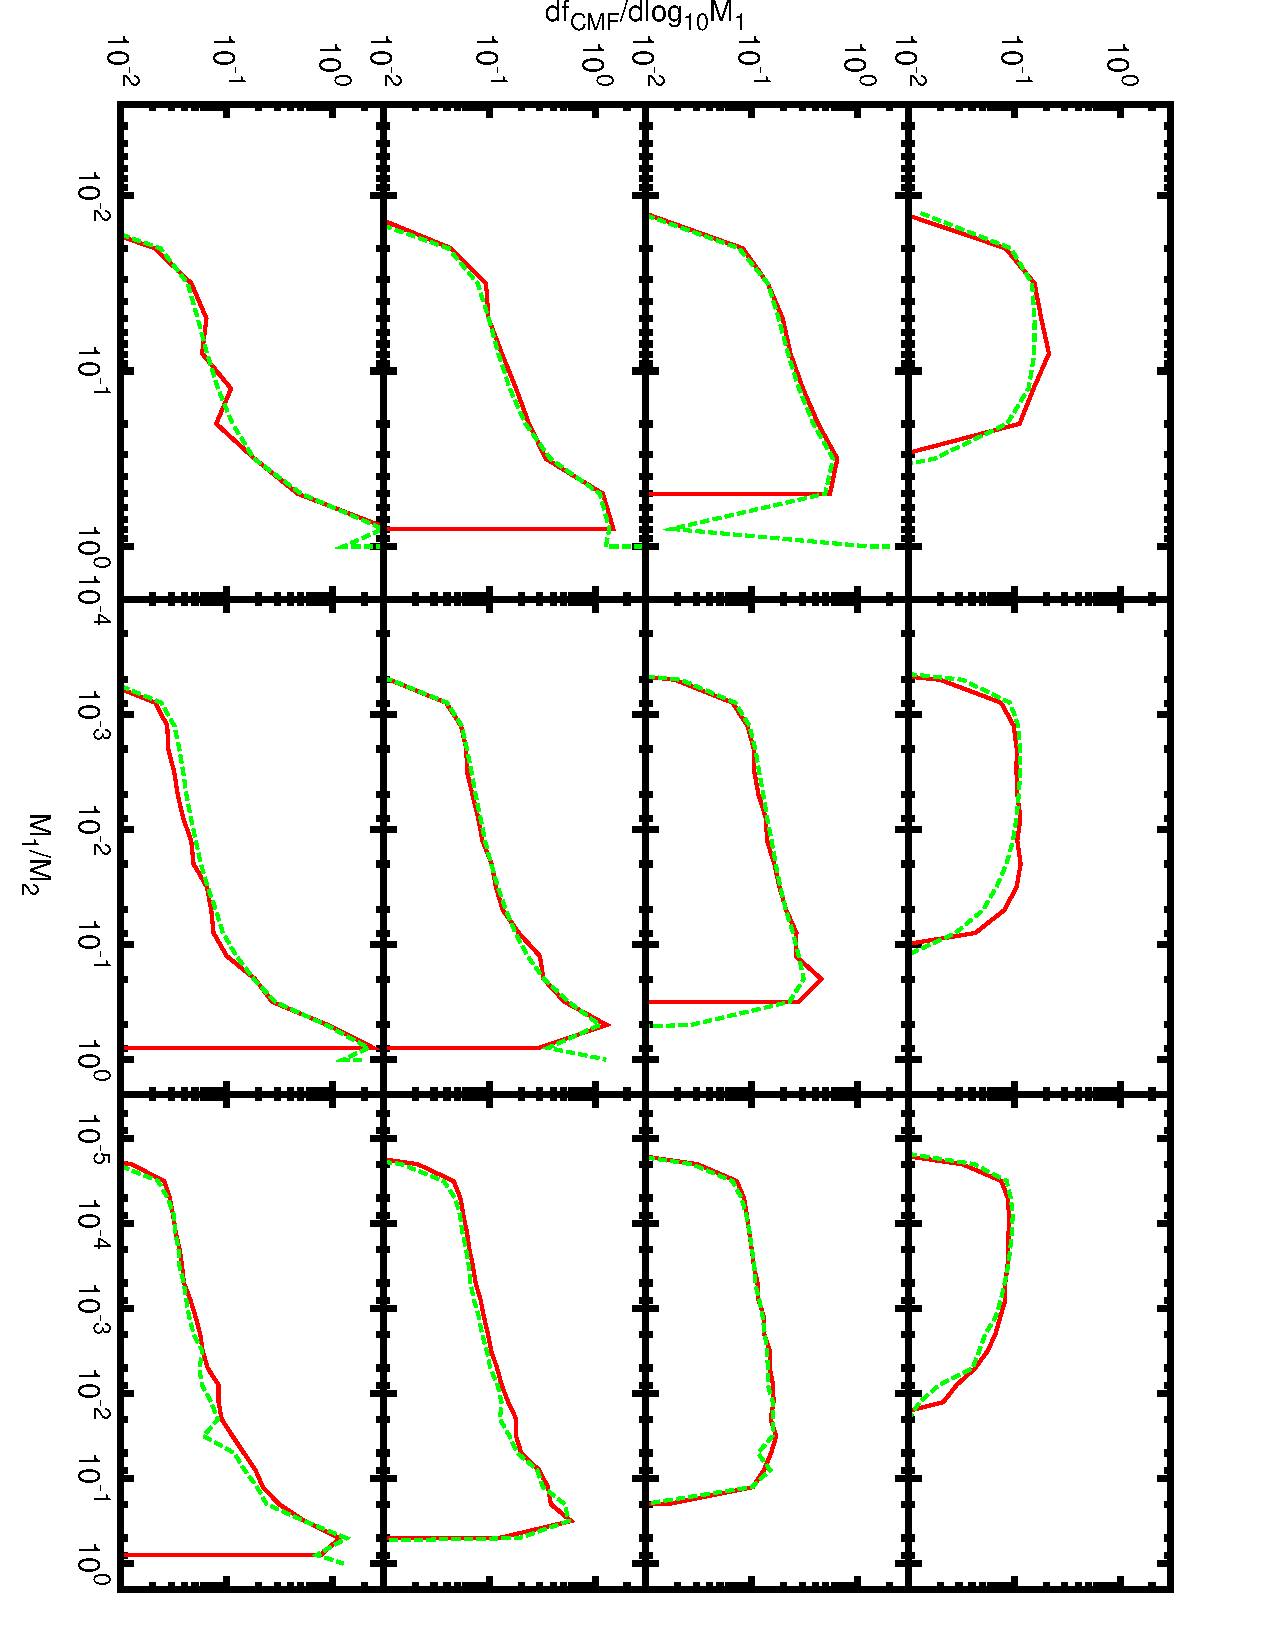
\includegraphics[height=160mm,angle=90]{../plots/progenitorMassFunction.pdf}
 \end{center}
 \caption{Progenitor mass functions at redshifts $z=0.5$, 1, 2 and 4 (bottom to top) for halos of mass $10^{12\pm0.151}$, $10^{13.5\pm0.151}$ and $10^{15\pm0.151}h^{-1}M_\odot$ (left to right) are shown. Green lines are measured from the Millennium Simulation, while red lines are computed using \glc's merger tree building routines (with the \cite{parkinson_generating_2008} branching algorithm and the \cite{cole_hierarchical_2000} tree building algorithm).}
 \label{fig:PCH_Progenitor_MFs}
\end{figure}

\subsubsection{Merger Tree Building}\label{sec:MergerTreeBuildMethod}

Additional methods for merger tree building can be added using the {\tt mergerTreeBuildMethod} directive. The directive should contain a single argument, giving the name of a subroutine to be called to initialize the method. For example, the {\tt Cole2000} method is described by a directive:
\begin{verbatim}
 !# <mergerTreeBuildMethod>
 !#  <unitName>Merger_Tree_Build_Cole2000_Initialize</unitName>
 !# </mergerTreeBuildMethod>
\end{verbatim}
Here, {\tt Merger\_Tree\_Build\_Cole2000\_Initialize} is the name of a subroutine which will be called to initialize the method. The initialization subroutine must have the following form:
\begin{verbatim}
 subroutine Method_Initialize(mergerTreeBuildMethod,Merger_Tree_Build)
    type(varying_string),          intent(in)    :: mergerTreeBuildMethod
    procedure(),          pointer, intent(inout) :: Merger_Tree_Build
    
    if (mergerTreeBuildMethod == 'myMethod') then
       Merger_Tree_Build => My_Do_Tabulate
       .
       .
       .
    end if
    return
  end subroutine Method_Initialize
\end{verbatim}
where {\tt myMethod} is the name of this method as will be specified by the {\tt mergerTreeBuildMethod} input parameter. The procedure pointer {\tt Merger\_Tree\_Build} must build and return a merger tree given the a base node as described below. The initialization subroutine should perform any other tasks required to initialize the module (such as reading parameters etc.).

\begin{verbatim}
  subroutine Merger_Tree_Build_Do(thisTree)
    type(mergerTree), intent(inout) :: thisTree
    .
    .
    .
    return
  end subroutine Merger_Tree_Build_Do
\end{verbatim}
and should return a full merger tree in {\tt thisTree} built from the base node which will already be set in {\tt thisTree}. The tree must have at least masses, times and parent/child/sibling links created. Other properties (e.g. spins) can be optionally included also.

Currently defined merger tree building methods are:
\begin{description}
 \item [{\tt Cole2000}] Uses the \cite{cole_hierarchical_2000} merger tree building algorithm.
\end{description}

\subsubsection{Merger Tree Construction}

Additional methods for merger tree construction can be added using the {\tt mergerTreeConstructMethod} directive. The directive should contain a single argument, giving the name of a subroutine to be called to initialize the method. For example, the {\tt build} method is described by a directive:
\begin{verbatim}
 !# <mergerTreeConstructMethod>
 !#  <unitName>Merger_Tree_Build_Initialize</unitName>
 !# </mergerTreeConstructMethod>
\end{verbatim}
Here, {\tt Merger\_Tree\_Build\_Initialize} is the name of a subroutine which will be called to initialize the method. The initialization subroutine must have the following form:
\begin{verbatim}
   subroutine Method_Initialize(mergerTreeConstructMethod,Merger_Tree_Construct)
    type(varying_string),          intent(in)    :: mergerTreeConstructMethod
    procedure(),          pointer, intent(inout) :: Merger_Tree_Construct
    
    if (mergerTreeConstructMethod.eq.'myMethod') then
       Merger_Tree_Construct => My_Do_Tabulate
       .
       .
       .
    end if
    return
  end subroutine Method_Initialize
\end{verbatim}
where {\tt myMethod} is the name of this method as will be specified by the {\tt mergerTreeConstructMethod} input parameter. The procedure pointer {\tt Merger\_Tree\_Construct} must be set to point to a function which returns a fully constructed merger tree as described below. The initialization subroutine should perform any other tasks required to initialize the module (such as reading parameters etc.).

The construction subroutine should have the following form:
\begin{verbatim}
  subroutine Merger_Tree_Construct_Do(thisTree)
    type(mergerTree), intent(inout) :: thisTree
    .
    .
    .
    return
  end subroutine Merger_Tree_Construct_Do
\end{verbatim}
and should return a full merger tree in {\tt thisTree}. The tree must have at least masses, times and parent/child/sibling links created. Other properties (e.g. spins) can be optionally included also.

Currently defined merger tree building methods are:
\begin{description}
 \item [{\tt build}] Generates a set of halo masses distributed between {\tt mergerTreeBuildHaloMassMinimum} and {\tt mergerTreeBuildHaloMassMaximum} (with {\tt mergerTreeBuildTreesPerDecade} halos per decade of mass) at redshift {\tt mergerTreeBuildTreesBaseRedshift} and then uses the selected merger tree build method (see \S\ref{sec:MergerTreeBuildMethod}) to build trees from these base nodes;
 \item [{\tt read}] Reads merger tree data from an HDF5 file (see \S\ref{sec:MergerTreeFiles}). The file to read is specified by the {\tt [mergerTreeReadFileName]} parameter.
\end{description}

\subsubsection{Population III Supernovae}

Additional methods for Population III supernovae can be added using the {\tt supernovaePopIIIMethod} directive. The directive should contain a single argument, giving the name of a subroutine to be called to initialize the method. For example, the {\tt Heger + Woosley} method is described by a directive:
\begin{verbatim}
  !# <supernovaePopIIIMethod>
  !#  <unitName>Supernovae_Population_III_HegerWoosley_Initialize</unitName>
  !# </supernovaePopIIIMethod>
\end{verbatim}
Here, {\tt Supernovae\_Population\_III\_HegerWoosley\_Initialize} is the name of a subroutine which will be called to initialize the method. The initialization subroutine must have the following form:
\begin{verbatim}
  subroutine Method_Initialize(supernovaePopIIIMethod,SNePopIII_Cumulative_Energy_Get)
    implicit none
    type(varying_string),          intent(in)    :: supernovaePopIIIMethod
    procedure(),          pointer, intent(inout) :: SNePopIII_Cumulative_Energy_Get
    
    if (supernovaePopIIIMethod == 'myMethod') then
       SNePopIII_Cumulative_Energy_Get => My_SNePopIII_Cumulative_Energy_Get
       .
       .
       .
    end if
    return
  end subroutine Method_Initialize
\end{verbatim}
where {\tt myMethod} is the name of this method as will be specified by the {\tt supernovaePopIIIMethod} input parameter. The procedure pointer {\tt SNePopIII\_Cumulative\_Energy\_Get} must be set to point to a function which returns the cumulative energy input from Population III supernovae as described below. The initialization subroutine should perform any other tasks required to initialize the module (such as reading parameters etc.).

The functions must have the form:
\begin{verbatim}
   double precision function PopIII_Cumulative_Energy(initialMass,age,metallicity)
    implicit none
    double precision, intent(in) :: initialMass,age,metallicity
    .
    .
    .
    return
   end function PopIII_Cumulative_Energy 
\end{verbatim}
This function must return the cumulative energy (in $M_\odot$ (km/s)$^2$) from Population III supernovae resulting from a star with given {\tt initialMass} and {\tt metallicity} after a time {\tt age}.

Currently defined transfer function methods are:
\begin{description}
 \item [{\tt Heger + Woosley}] Computes the energy input from the pair-instability results of \cite{heger_nucleosynthetic_2002}.
\end{description}

\subsubsection{Primordial Power Spectrum}

Additional methods for the primordial power spectrum can be added using the {\tt powerSpectrumMethod} directive. The directive should contain a single argument, giving the name of a subroutine to be called to initialize the method. For example, the {\tt power law} method is described by a directive:
\begin{verbatim}
  !# <powerSpectrumMethod>
  !#  <unitName>CDM_Primordial_Power_Spectrum_Power_Law_Initialize</unitName>
  !# </powerSpectrumMethod>
\end{verbatim}
Here, {\tt CDM\_Primordial\_Power\_Spectrum\_Power\_Law\_Initialize} is the name of a subroutine which will be called to initialize the method. The initialization subroutine must have the following form:
\begin{verbatim}
  subroutine Method_Initialize(powerSpectrumMethod,Power_Spectrum_Tabulate)
    implicit none
    type(varying_string),          intent(in)    :: powerSpectrumMethod
    procedure(),          pointer, intent(inout) :: Power_Spectrum_Tabulate
    
    if (powerSpectrumMethod.eq.'myMethod') then
       Power_Spectrum_Tabulate => My_Do_Tabulate
       .
       .
       .
    end if
    return
  end subroutine Method_Initialize
\end{verbatim}
where {\tt myMethod} is the name of this method as will be specified by the {\tt powerSpectrumMethod} input parameter. The procedure pointer {\tt Power\_Spectrum\_Tabulate} must be set to point to a subroutine which tabulates the power spectrum as described below. The initialization subroutine should perform any other tasks required to initialize the module (such as reading parameters etc.).

The tabulation subroutine must have the form:
\begin{verbatim}
   subroutine Power_Spectrum_Tabulate(wavenumber,powerSpectrumNumberPoints,powerSpectrumLogWavenumber,powerSpectrumLogP)
    implicit none
    double precision,                            intent(in)    :: wavenumber
    double precision, allocatable, dimension(:), intent(inout) :: powerSpectrumLogWavenumber,powerSpectrumLogP
    integer,                                     intent(out)   :: powerSpectrumNumberPoints
    .
    .
    .
    return
   end subroutine Power_Spectrum_Tabulate
\end{verbatim}
The subroutine must tabulate the natural log of the power spectrum in array {\tt powerSpectrumLogP()} as a function of the natural log of wavenumber {\tt powerSpectrumLogWavenumber()} (these arrays must be allocated to the correct size, and may be prevously allocated, therefore requiring a deallocation). The number of tabulated points should be returned in {\tt powerSpectrumNumberPoints}. The subroutine should ensure that the currently requested {\tt wavenumber} is within the range of the tabulated function (preferably with some buffer).

Currently defined power spectrum methods are:
\begin{description}
 \item [{\tt power law}] The power spectrum is assumed to be a power law, possibly with a running index. It is defined by
\begin{equation}
 P(k)\propto k^{n_{\rm s} + \ln(k/k_{\rm ref}) [\d n /\d\ln k]},
\end{equation}
where the parameters are specified by input parameters $n_{\rm s}\equiv${\tt powerSpectrumIndex}, $k_{\rm ref}\equiv${\tt powerSpectrumReferenceWavenumber} and $\d n / \d \ln k \equiv${\tt powerSpectrumRunning}.
\end{description}

\subsubsection{Satellite Merging Mass Movements}

Additional methods for the satellite merging mass movements can be added using the {\tt satelliteMergingMassMovementsMethod} directive. The directive should contain a single argument, giving the name of a subroutine to be called to initialize the method. For example, the {\tt simple} method is described by a directive:
\begin{verbatim}
 !# <satelliteMergingMassMovementsMethod>
 !#  <unitName>Satellite_Merging_Mass_Movements_Simple_Initialize</unitName>
 !# </satelliteMergingMassMovementsMethod>
\end{verbatim}
Here, {\tt Satellite\_Merging\_Mass\_Movements\_Simple\_Initialize} is the name of a subroutine which will be called to initialize the method. The initialization subroutine must have the following form:
\begin{verbatim}
  subroutine Method_Initialize(satelliteMergingMassMovementsMethod,Satellite_Merging_Mass_Movement_Get)
    implicit none
    type(varying_string),          intent(in)    :: satelliteMergingMassMovementsMethod
    procedure(),          pointer, intent(inout) :: Satellite_Merging_Mass_Movement_Get
    
    if (satelliteMergingMassMovementsMethod == 'simple') Satellite_Merging_Mass_Movement_Get => My_Method_Get
    return
  end subroutine Method_Initialize
\end{verbatim}
where {\tt myMethod} is the name of this method as will be specified by the {\tt satelliteMergingMassMovementsMethod} input parameter. The procedure pointer {\tt Satellite\_Merging\_Mass\_Movement\_Get} must be set to point to a function which sets the mass movement descriptors as described below. The initialization subroutine should perform any other tasks required to initialize the module (such as reading parameters etc.).

The mass movement subroutine must have the form:
\begin{verbatim}
  subroutine My_Method_Get(thisNode,gasMovesTo,starsMoveTo,hostGasMovesTo,hostStarsMoveTo)
    implicit none
    type(treeNode), intent(inout), pointer  :: thisNode
    integer,        intent(out)             :: gasMovesTo,starsMoveTo,hostGasMovesTo,hostStarsMoveTo
    .
    .
    .
    return
  end subroutine My_Method_Get
\end{verbatim}
The subroutine must return values for each of the ``{\tt MoveTo}'' descriptors to specify where stars and gas from {\tt thisNode} and {\tt thisNode}'s host node should move to in the host. Allowed values are:
\begin{description}
 \item [{\tt movesToDisk}] The material in question moves to the disk of the host node;
 \item [{\tt movesToSpheroid}] The material in question moves to the spheroid of the host node;
 \item [{\tt doesNotMove}] The material in question does not move (allowed only for host node descriptors).
\end{description}

Currently defined satellite merger mass movement methods are:
\begin{description}
 \item [{\tt simple}] If the baryonic mass of the satellite exceeds a fraction {\tt majorMergerMassRatio} of the baryonic mass of the host then all material is moved to the spheroid of the host. Otherwise, satellite gas moves to the host disk, satellite stars move to the host spheroid and host material does not move.
\end{description}

\subsubsection{Satellite Merging Remnant Sizes}\label{sec:satelliteMergerMassMovementMethod}

Additional methods for the satellite merging remnant sizes can be added using the {\tt satelliteMergingRemnantSizeMethod} directive. The directive should contain a single argument, giving the name of a subroutine to be called to initialize the method. For example, the {\tt Cole2000} method is described by a directive:
\begin{verbatim}
 !# <satelliteMergingRemnantSizeMethod>
 !#  <unitName>Satellite_Merging_Remnant_Sizes_Cole2000_Initialize</unitName>
 !# </satelliteMergingRemnantSizeMethod>
\end{verbatim}
Here, {\tt Satellite\_Merging\_Remnant\_Sizes\_Cole2000\_Initialize} is the name of a subroutine which will be called to initialize the method. The initialization subroutine must have the following form:
\begin{verbatim}
  subroutine Method_Initialize(satelliteMergingRemnantSizeMethod,Satellite_Merging_Remnant_Size_Do)
    implicit none
    type(varying_string),          intent(in)    :: satelliteMergingRemnantSizeMethod
    procedure(),          pointer, intent(inout) :: Satellite_Merging_Remnant_Size_Do
    
    if (satelliteMergingRemnantSizeMethod == 'myMethod') Satellite_Merging_Remnant_Size_Do => My_Method_Do
    return
  end subroutine Method_Initialize
\end{verbatim}
where {\tt myMethod} is the name of this method as will be specified by the {\tt satelliteMergingRemnantSizeMethod} input parameter. The procedure pointer {\tt Satellite\_Merging\_Remnant\_Size\_Do} must be set to point to a function which computes the size of the merger remnant and stores the properties (e.g. radius, circular velocity and specific angular momentum at the half-mass radius) of the \emph{host} node. The initialization subroutine should perform any other tasks required to initialize the module (such as reading parameters etc.).

The remnant size subroutine must have the form:
\begin{verbatim}
  subroutine My_Method_Do(thisNode)
    implicit none
    type(treeNode), intent(inout), pointer  :: thisNode
    .
    .
    .
    return
  end subroutine My_Method_Do
\end{verbatim}
The subroutine must compute the properties of the merger remnant. Typically these are stored in the {\tt Satellite\_Merging\_Remnant\_Sizes\_Properties} module for later retrieval by the appropriate component.

Currently defined satellite merger remnant size methods are:
\begin{description}
 \item [{\tt null}] This is a null method which does nothing. It is useful for runs where no baryonic components are included (e.g. for studying dark matter only).
 \item [{\tt Cole2000}] Implements the algorithm of \cite{cole_hierarchical_2000} to compute the remnant size. The orbital energy assumed can be adjusted using the {\tt mergerRemnantSizeOrbitalEnergy} parameter, which is equivalent to the $f_{\rm orbit}$ parameter of \cite{cole_hierarchical_2000}.
\end{description}

\subsubsection{Satellite Merging Timescales}

Additional methods for the satellite merging timescales can be added using the {\tt satelliteMergingMethod} directive. The directive should contain a single argument, giving the name of a subroutine to be called to initialize the method. For example, the {\tt Lacey-Cole} method is described by a directive:
\begin{verbatim}
  !# <satelliteMergingMethod>
  !#  <unitName>Satellite_Time_Until_Merging_Lacey_Cole_Initialize</unitName>
  !# </satelliteMergingMethod>
\end{verbatim}
Here, {\tt Satellite\_Time\_Until\_Merging\_Lacey\_Cole\_Initialize} is the name of a subroutine which will be called to initialize the method. The initialization subroutine must have the following form:
\begin{verbatim}
  subroutine Method_Initialize(satelliteMergingMethod,Satellite_Time_Until_Merging)
    implicit none
    type(varying_string),          intent(in)    :: satelliteMergingMethod
    procedure(),          pointer, intent(inout) :: Satellite_Time_Until_Merging
    
    if (satelliteMergingMethod == 'myMethod') Satellite_Time_Until_Merging => My_Method_Procedure
    return
  end subroutine Method_Initialize
\end{verbatim}
where {\tt myMethod} is the name of this method as will be specified by the {\tt satelliteMergingMethod} input parameter. The procedure pointer {\tt Satellite\_Time\_Until\_Merging} must be set to point to a function which returns the time until merging as described below. The initialization subroutine should perform any other tasks required to initialize the module (such as reading parameters etc.).

The merging timescale function must have the form:
\begin{verbatim}
 double precision function Satellite_Time_Until_Merging(thisNode)
    implicit none
    type(treeNode),   pointer, intent(inout) :: thisNode
    .
    .
    .
    return
 end function Satellite_Time_Until_Merging
\end{verbatim}
The function must return the merging timescale for {\tt thisNode} orbitting in {\tt thisNode\%parentNode} in units of Gyr.

Currently defined satellite virial orbit methods are:
\begin{description}
 \item [\hyperlink{satellites.merging.dynamical_friction.timescale.Lacey-Cole.F90:dynamical_friction_lacey_cole:satellite_time_until_merging_lacey_cole}{{\tt Lacey-Cole}}] Computes the merging timescale using the method of \cite{lacey_merger_1993}.
 \item [\hyperlink{satellites.merging.dynamical_friction.timescale.Jiang2008.F90:dynamical_friction_jiang2008:satellite_time_until_merging_jiang2008}{{\tt Jiang2008}}] Computes the merging timescale using the method of \cite{jiang_fitting_2008}.
 \item [\hyperlink{satellites.merging.dynamical_friction.timescale.Boylan-Kolchin2008.F90:dynamical_friction_boylankolchin2008:satellite_time_until_merging_boylankolchin2008}{{\tt BoylanKolchin2008}}] Computes the merging timescale using the method of \cite{boylan-kolchin_dynamical_2008}.
\end{description}

\subsubsection{Satellite Virial Orbits}

Additional methods for the satellite virial orbits (i.e. orbital parameters at virial radius crossing) can be added using the {\tt virialOrbitsMethod} directive. The directive should contain a single argument, giving the name of a subroutine to be called to initialize the method. For example, the {\tt Benson2005} method is described by a directive:
\begin{verbatim}
  !# <virialOrbitsMethod>
  !#  <unitName>Virial_Orbital_Parameters_Benson2005_Initialize</unitName>
  !# </virialOrbitsMethod>
\end{verbatim}
Here, {\tt Virial\_Orbital\_Parameters\_Benson2005\_Initialize} is the name of a subroutine which will be called to initialize the method. The initialization subroutine must have the following form:
\begin{verbatim}
  subroutine Method_Initialize(virialOrbitsMethod,Virial_Orbital_Parameters_Get)
    implicit none
    type(varying_string),          intent(in)    :: virialOrbitsMethod
    procedure(),          pointer, intent(inout) :: Virial_Orbital_Parameters_Get
    
    if (virialOrbitsMethod.eq.'myMethod') Virial_Orbital_Parameters_Get => My_Method_Procedure
    return
  end subroutine Method_Initialize
\end{verbatim}
where {\tt myMethod} is the name of this method as will be specified by the {\tt virialOrbitsMethod} input parameter. The procedure pointer {\tt Virial\_Orbital\_Parameters\_Get} must be set to point to a subroutine which returns orbital parameters as described below. The initialization subroutine should perform any other tasks required to initialize the module (such as reading parameters etc.).

The orbital parameter subroutine must have the form:
\begin{verbatim}
  subroutine Virial_Orbital_Parameters(thisNode,acceptUnboundOrbits,velocityRadial,velocityTangential,angularMomentum&
       &,orbitalEnergy,eccentricity,semimajorAxis)
    implicit none
    type(treeNode),   intent(inout), pointer  :: thisNode
    logical,          intent(in)              :: acceptUnboundOrbits
    double precision, intent(out),   optional :: velocityRadial,velocityTangential,angularMomentum,orbitalEnergy,eccentricity&
         &,semimajorAxis

    return
  end subroutine Virial_Orbital_Parameters
\end{verbatim}
The subroutine must return orbital parameters for {\tt thisNode} orbitting in {\tt thisNode\%parentNode}, for whichever of the arguments are present in the subroutine call. If {\tt acceptUnboundOrbits} is true, then unbound orbits may be returned, otherwise, the routine must ensure that the returned orbit is bound. Velocities should be return in units of km/s, lengthscales in units of Mpc.

Currently defined satellite virial orbit methods are:
\begin{description}
 \item [\hyperlink{satellites.merging.virial_orbits.Benson2005.F90:virial_orbits_benson2005:virial_orbital_parameters_benson2005}{{\tt Benson2005}}] The orbital parameters are select from the distribution found by \cite{benson_orbital_2005}.
\end{description}

\subsubsection{Star Formation Feedback in Disks/Spheroids}

Additional methods for computing feedback from star formation in disks/spheroids can be added using the {\tt starFormationFeedback[Disks|Spheroids]Method} directive. The directive should contain a single argument, giving the name of a subroutine to be called to initialize the method. For example, the {\tt power law} method is described by a directive:
\begin{verbatim}
 !# <starFormationFeedbackSpheroidsMethod>
 !#  <unitName>Star_Formation_Feedback_Spheroids_Power_Law_Initialize</unitName>
 !# </starFormationFeedbackSpheroidsMethod>
\end{verbatim}
Here, {\tt Star\_Formation\_Feedback\_Spheroids\_Power\_Law\_Initialize} is the name of a subroutine which will be called to initialize the method. The initialization subroutine must have the following form:
\begin{verbatim}
  subroutine Method_Initialize(starFormationFeedbackDisksMethod,Star_Formation_Feedback_Disk_Outflow_Rate_Get)
    implicit none
    type(varying_string),          intent(in)    :: starFormationFeedbackDisksMethod
    procedure(),          pointer, intent(inout) :: Star_Formation_Feedback_Disk_Outflow_Rate_Get
    
    if (starFormationFeedbackDisksMethod == 'myMethod') Star_Formation_Feedback_Disk_Outflow_Rate_Get => My_Star_Formation_Feedback_Disk_Outflow_Rate_Get
    return
  end subroutine Method_Initialize
\end{verbatim}
where {\tt myMethod} is the name of this method as will be specified by the {\tt starFormationFeedback[Disks|Spheroids]Method} input parameter. The procedure pointer {\tt Star\_Formation\_Feedback\_Disk\_Outflow\_Rate\_Get} (or {\tt Star\_Formation\_Feedback\_Spheroid\_Outflow\_Rate\_Get} for the spheroid case) must be set to point to a function which returns the mass outflow rate due to star formation as described below. The initialization subroutine should perform any other tasks required to initialize the module (such as reading parameters etc.).

The outflow rate function must have the form:
\begin{verbatim}
 double precision function Star_Formation_Feedback_Outflow_Rate_Get(thisNode,starFormationRate,energyInputRate)
    implicit none
    type(treeNode),   intent(inout), pointer :: thisNode
    double precision, intent(in)             :: starFormationRate,energyInputRate
    .
    .
    .
    return
 end function Star_Formation_Feedback_Outflow_Rate_Get
\end{verbatim}
The function must return the mass outflow rate (in $M_\odot$ Gyr$^{-1}$) for {\tt thisNode}.

Currently defined star formation feedback methods are:
\begin{description}
 \item [\hyperlink{star_formation.feedback.spheroids.power_law.F90:star_formation_feedback_spheroids_power_law:star_formation_feedback_spheroid_outflow_rate_power_law}{{\tt power law}}] The outflow rate is given by
\begin{equation}
 \dot{M}_{\rm outflow} = \left({V_{\rm outflow} \over V}\right)^{\alpha_{\rm outflow}} {\dot{E} \over E_{\rm canonical}},
\end{equation}
where $V_{\rm outflow}=${\tt [disk|spheroid]OutflowVelocity} (in km/s) and $\alpha_{\rm outflow}=${\tt [disk|spheroid]OutflowVelocity} are input parameters, $V$ is the characteristic velocity of the component, $\dot{E}$ is the rate of energy input from stellar populations and $E_{\rm canonical}$ is the total energy input by a canonical stellar population normalized to $1 M_\odot$ after infinite time.
\end{description}

\subsubsection{Star Formation Timescale in Disks/Spheroids}

Additional methods for computing star formation timescales in disks/spheroids can be added using the {\tt starFormationTimescale[Disks|Spheroids]Method} directive. The directive should contain a single argument, giving the name of a subroutine to be called to initialize the method. For example, the {\tt dynamical time} method is described by a directive:
\begin{verbatim}
 !# <starFormationTimescaleDisksMethod>
 !#  <unitName>Star_Formation_Timescale_Disks_Dynamical_Time_Initialize</unitName>
 !# </starFormationTimescaleDisksMethod>
\end{verbatim}
Here, {\tt Star\_Formation\_Timescale\_Disks\_Dynamical\_Time\_Initialize} is the name of a subroutine which will be called to initialize the method. The initialization subroutine must have the following form:
\begin{verbatim}
  subroutine Method_Initialize(starFormationTimescaleDisksMethod,Star_Formation_Timescale_Disk_Get)
    implicit none
    type(varying_string),          intent(in)    :: starFormationTimescaleDisksMethod
    procedure(),          pointer, intent(inout) :: Star_Formation_Timescale_Disk_Get
    
    if (starFormationTimescaleDisksMethod == 'myMethod') Star_Formation_Timescale_Disk_Get => My_Method_Get_Procedure
    return
  end subroutine Method_Initialize
\end{verbatim}
where {\tt myMethod} is the name of this method as will be specified by the {\tt starFormationTimescale[Disks|Spheroids]Method} input parameter. The procedure pointer {\tt Star\_Formation\_Timescale\_Disk\_Get} (or {\tt Star\_Formation\_Timescale\_Spheroid\_Get} for the spheroid case) must be set to point to a function which returns the timescale for star formation as described below. The initialization subroutine should perform any other tasks required to initialize the module (such as reading parameters etc.).

The star formation timescale function must have the form:
\begin{verbatim}
 double precision function Star_Formation_Timescale_Get(thisNode)
    implicit none
    type(treeNode), intent(in) :: thisNode
    .
    .
    .
    return
 end function Star_Formation_Timescale_Get
\end{verbatim}
The function must return the star formation timescale (in units of Gyr) for {\tt thisNode}.

Currently defined star formation timescale methods are:
\begin{description}
 \item [\hyperlink{star_formation.timescales.disks.dynamical_time.F90:star_formation_timescale_disks_dynamical_time:star_formation_timescale_disk_dynamical_time}{{\tt dynamical time}}]  The timescale is given by
\begin{equation}
 \tau_\star = \epsilon_\star^{-1} \tau_{\rm dynamical, [disk|spheroid]} \left( {V_{\rm [disk|spheroid]} \over 200\hbox{km/s}} \right)^{\alpha_\star},
\end{equation}
where $\epsilon_\star$(={\tt starFormation[Disk|Spheroid]Efficiency}) is a star formation efficiency and $\alpha_\star$(={\tt starFormation[Disk|Spheroid]VelocityExponent}) controls the scaling with velocity. Note that $\tau_{\rm dynamical,[disk|spheroid]}=R_{\rm [disk|spheroid]}/V_{\rm [disk|spheroid]}$ where the radius and velocity are whatever characteristic values returned by the disk/spheroid method. This scaling is functionally similar to that adopted by \cite{cole_hierarchical_2000}, but that they specifically used the half-mass radius and circular velocity at that radius.
\end{description}

\subsubsection{Stellar Astrophysics}

Additional methods for stellar astrophysical properties can be added using the {\tt stellarAstrophysicsMethod} directive. The directive should contain a single argument, giving the name of a subroutine to be called to initialize the method. For example, the {\tt file} method is described by a directive:
\begin{verbatim}
  !# <stellarAstrophysicsMethod>
  !#  <unitName>Stellar_Astrophysics_File_Initialize</unitName>
  !# </stellarAstrophysicsMethod>
\end{verbatim}
Here, {\tt Stellar\_Astrophysics\_File\_Initialize} is the name of a subroutine which will be called to initialize the method. The initialization subroutine must have the following form:
\begin{verbatim}
  subroutine Method_Initialize(stellarAstrophysicsMethod,Star_Ejected_Mass_Get,Star_Initial_Mass_Get,Star_Metal_Yield_Mass_Get,Star_Lifetime_Get)
    implicit none
    type(varying_string),          intent(in)    :: stellarAstrophysicsMethod
    procedure(),          pointer, intent(inout) :: Star_Ejected_Mass_Get,Star_Initial_Mass_Get,Star_Metal_Yield_Mass_Get,Star_Lifetime_Get
    
    if (stellarAstrophysicsMethod == 'myMethod') then
      Star_Ejected_Mass_Get     => My_Star_Ejected_Mass
      Star_Initial_Mass_Get     => My_Star_Initial_Mass
      Star_Metal_Yield_Mass_Get => My_Star_Metal_Yield_Mass
      Star_Lifetime_Get         => My_Star_Lifetime
    end if
    return
  end subroutine Method_Initialize
\end{verbatim}
where {\tt myMethod} is the name of this method as will be specified by the {\tt stellarAstrophysicsMethod} input parameter. The procedure pointers must be set to point to functions which return stellar properties as described below. The initialization subroutine should perform any other tasks required to initialize the module (such as reading parameters etc.).

The ejected mass, metal yield and lifetime functions must have the form:
\begin{verbatim}
 double precision function Star_Property(initialMass,metallicity)
    implicit none
    double precision, intent(in) :: initialMass,metallicity
    .
    .
    .
    return
 end function Star_Property
\end{verbatim}
These functions must return the total ejected mass (in $M_\odot$), total metal yield (in $M_\odot$) and lifetime (in Gyr) for a star of the specified {\tt initialMass} and {\tt metallicity}.

The initial mass function must have the form:
\begin{verbatim}
 double precision function Star_Initial_Mass(lifetime,metallicity)
    implicit none
    double precision, intent(in) :: lifetime,metallicity
    .
    .
    .
    return
 end function Star_Initial_Mass
\end{verbatim}
and should return the initial mass (in $M_\odot$) of a star of given {\tt lifetime} (specified in Gyr) and {\tt metallicity}.

Currently defined stellar astrophysics methods are:
\begin{description}
 \item [{\tt file}] Stellar properties are read from an XML file and interpolated. The structure of the XML file is described in \S\ref{sec:StellarAstrophysicsFile}.
\end{description}

\subsubsection{Stellar Population Properties}

Additional methods for computing properties of stellar populations can be added using the {\tt stellarPopulationPropertiesMethod} directive. The directive should contain a single argument, giving the name of a subroutine to be called to initialize the method. For example, the {\tt instantaneous} method is described by a directive:
\begin{verbatim}
 !# <stellarPopulationPropertiesMethod>
 !#  <unitName>Stellar_Population_Properties_Instantaneous_Initialize</unitName>
 !# </stellarPopulationPropertiesMethod>
\end{verbatim}
Here, {\tt Stellar\_Population\_Properties\_Instantaneous\_Initialize} is the name of a subroutine which will be called to initialize the method. The initialization subroutine must have the following form:
\begin{verbatim}
  subroutine Method_Initialize(stellarPopulationPropertiesMethod,Stellar_Population_Properties_Rates_Get,Stellar_Population_Properties_History_Count_Get)
    implicit none
    type(varying_string),          intent(in)    :: stellarPopulationPropertiesMethod
    procedure(),          pointer, intent(inout) :: Stellar_Population_Properties_Rates_Get,Stellar_Population_Properties_History_Count_Get
    
    if (stellarPopulationPropertiesMethod == 'myMethod') then
       Stellar_Population_Properties_Rates_Get         => My_Method_Rates_Get_Procedure
       Stellar_Population_Properties_History_Count_Get => My_Method_History_Count_Get_Procedure
    end if
    return
  end subroutine Method_Initialize
\end{verbatim}
where {\tt myMethod} is the name of this method as will be specified by the {\tt stellarPopulationPropertiesMethod} input parameter. The procedure pointer {\tt Stellar\_Population\_Properties\_Rates\_Get} must be set to point to a subroutine which returns properties of a stellar population as described below, while the {\tt My\_Method\_History\_Count\_Get\_Procedure} procedure pointer must be set to point to a function which returns the number of histories that will be required by this method. The initialization subroutine should perform any other tasks required to initialize the module (such as reading parameters etc.).

The stellar populations properties subroutine must have the form:
\begin{verbatim}
 subroutine Stellar_Population_Properties_Rates(starFormationRate,fuelAbundances,thisNode,thisHistory,stellarMassRate&
       &,stellarAbundancesRates,stellarLuminositiesRates,fuelMassRate,fuelAbundancesRates,energyInputRate)
    implicit none
    implicit none
    double precision,          intent(out)                 :: stellarMassRate,fuelMassRate,energyInputRate
    type(abundancesStructure), intent(out)                 :: stellarAbundancesRates,fuelAbundancesRates
    double precision,          intent(out),   dimension(:) :: stellarLuminositiesRates
    double precision,          intent(in)                  :: starFormationRate
    type(abundancesStructure), intent(in)                  :: fuelAbundances
    type(treeNode),            intent(inout), pointer      :: thisNode
    type(history),             intent(inout)               :: thisHistory
    .
    .
    .
    return
 end subroutine Stellar_Population_Properties_Rates
\end{verbatim}
The subroutine is given the {\tt starFormationRate} (in $M_\odot$ Gyr$^{-1}$) in {\tt thisNode}. Any history information required by this method must be passed in via the {\tt history} argument. Stars are forming from fuel material with composition specified by {\tt fuelAbundances}. The subroutine must return the rates of change of stellar and fuel mass (in $M_\odot$ Gyr$^{-1}$) in {\tt stellarMassRate} and {\tt fuelMassRate} respectively, and the corresponding rates (also in $M_\odot$ Gyr$^{-1}$) of abundance change in {\tt stellarAbundancesRates} and {\tt fuelAbundancesRates} respectively. Finally, it should return rates of change (in $L_{\rm AB}$ Gyr$^{-1}$) of stellar luminosities for all requested output bands in {\tt stellarLuminositiesRates}. Additionally, the rate of energy input from stellar populations must be returned in {\tt energyInputRate}.

The history function function must have the form
\begin{verbatim}
 integer function Stellar_Population_Properties_History_Count()
    implicit none
    .
    .
    return
 end function Stellar_Population_Properties_History_Count
\end{verbatim}
and should return the number of histories that will be required by this method.

Currently defined stellar population properties methods are:
\begin{description}
 \item [\hyperlink{stellar_populations.properties.instantaneous.F90:stellar_population_properties_instantaneous:stellar_population_properties_rates_instantaneous}{{\tt instantaneous}}] Computes stellar population properties using an instantaneous recyclying approximation.
\end{description}

\subsubsection{Stellar Feedback}

Additional methods for stellar feedback can be added using the {\tt stellarFeedbackMethod} directive. The directive should contain a single argument, giving the name of a subroutine to be called to initialize the method. For example, the {\tt standard} method is described by a directive:
\begin{verbatim}
  !# <stellarFeedbackMethod>
  !#  <unitName>Stellar_Feedback_Standard_Initialize</unitName>
  !# </stellarFeedbackMethod>
\end{verbatim}
Here, {\tt Stellar\_Feedback\_Standard\_Initialize} is the name of a subroutine which will be called to initialize the method. The initialization subroutine must have the following form:
\begin{verbatim}
  subroutine Method_Initialize(stellarFeedbackMethod,Stellar_Feedback_Cumulative_Energy_Input_Get)
    implicit none
    type(varying_string),          intent(in)    :: stellarFeedbackMethod
    procedure(),          pointer, intent(inout) :: Stellar_Feedback_Cumulative_Energy_Input_Get
    
    if (stellarFeedbackMethod == 'myMethod') then
       Stellar_Feedback_Cumulative_Energy_Input_Get => My_Stellar_Feedback_Cumulative_Energy_Input_Get
       .
       .
       .
    end if
    return
  end subroutine Method_Initialize
\end{verbatim}
where {\tt myMethod} is the name of this method as will be specified by the {\tt stellarFeedbackMethod} input parameter. The procedure pointer {\tt Stellar\_Feedback\_Cumulative\_Energy\_Input\_Get} must be set to point to a function which returns the cumulative energy input from stars as described below. The initialization subroutine should perform any other tasks required to initialize the module (such as reading parameters etc.).

The function must have the form:
\begin{verbatim}
   double precision function Stellar_Feedback_Cumulative_Energy_Input(initialMass,age,metallicity)
    implicit none
    double precision, intent(in) :: initialMass,age,metallicity
    .
    .
    .
    return
   end function Stellar_Feedback_Cumulative_Energy_Input 
\end{verbatim}
The function must return the cumulative energy input (in $M_\odot$ (km/s)$^2$ from stars of given {\tt initialMass} and {\tt metallicity} after a time {\tt age}.

Currently defined transfer function methods are:
\begin{description}
 \item [{\tt standard}] This method assumes that the energy input has contributions from stellar winds, Type Ia, Type II and Population III supernovae. The minimum mass required for a star to produce a Type II supernova is specified via {\tt initialMassForSupernovaeTypeII} (in $M_\odot$), while the energy per Type II or Ia supernova is specified via {\tt supernovaEnergy} (in ergs).
\end{description}

\subsubsection{Stellar Tracks}

Additional methods for stellar tracks can be added using the {\tt stellarTracksMethod} directive. The directive should contain a single argument, giving the name of a subroutine to be called to initialize the method. For example, the {\tt file} method is described by a directive:
\begin{verbatim}
  !# <stellarTracksMethod>
  !#  <unitName>Stellar_Tracks_Initialize_File</unitName>
  !# </stellarTracksMethod>
\end{verbatim}
Here, {\tt Stellar\_Tracks\_Initialize\_File} is the name of a subroutine which will be called to initialize the method. The initialization subroutine must have the following form:
\begin{verbatim}
  subroutine Method_Initialize(stellarTracksMethod,Stellar_Luminosity_Get,Stellar_Effective_Temperature_Get)
    implicit none
    type(varying_string),          intent(in)    :: stellarTracksMethod
    procedure(),          pointer, intent(inout) :: Stellar_Luminosity_Get,Stellar_Effective_Temperature_Get
    
    if (stellarTracksMethod == 'myMethod') then
       Stellar_Luminosity_Get            => My_Stellar_Luminosity_Get
       Stellar_Effective_Temperature_Get => My_Stellar_Effective_Temperature_Get
       .
       .
       .
    end if
    return
  end subroutine Method_Initialize
\end{verbatim}
where {\tt myMethod} is the name of this method as will be specified by the {\tt stellarTracksMethod} input parameter. The procedure pointers {\tt Stellar\_Luminosity\_Get} and {\tt Stellar\_Effective\_Temperature\_Get} must be set to point to functions which return the luminosity and effective temperatures of stars as described below. The initialization subroutine should perform any other tasks required to initialize the module (such as reading parameters etc.).

The functions must have the form:
\begin{verbatim}
   double precision function Stellar_Tracks_Function(initialMass,age,metallicity)
    implicit none
    double precision, intent(in) :: initialMass,age,metallicity
    .
    .
    .
    return
   end function Stellar_Tracks_Function 
\end{verbatim}
The luminosity function must return the bolometric luminosity (in $L_\odot$) of a star of given {\tt initialMass} and {\tt metallicity} after a time {\tt age}. The effective temperature function should give the effective temperature (in Kelvin) for the same star.

Currently defined stellar tracks methods are:
\begin{description}
 \item [{\tt file}] Stellar tracks are read from an HDF5 file and interpolated in. The structure of the HDF5 is described in \S\ref{sec:StellarTracksFile}.
\end{description}

\subsubsection{Stellar Winds}

Additional methods for stellar winds can be added using the {\tt stellarWindsMethod} directive. The directive should contain a single argument, giving the name of a subroutine to be called to initialize the method. For example, the {\tt Leitherer1992} method is described by a directive:
\begin{verbatim}
  !# <stellarWindsMethod>
  !#  <unitName>Stellar_Winds_Leitherer1992_Initialize</unitName>
  !# </stellarWindsMethod>
\end{verbatim}
Here, {\tt Stellar\_Winds\_Leitherer1992\_Initialize} is the name of a subroutine which will be called to initialize the method. The initialization subroutine must have the following form:
\begin{verbatim}
  subroutine Method_Initialize(stellarWindsMethod,Stellar_Winds_Mass_Loss_Rate_Get,Stellar_Winds_Terminal_Velocity_Get)
    implicit none
    type(varying_string),          intent(in)    :: stellarWindsMethod
    procedure(),          pointer, intent(inout) :: Stellar_Winds_Mass_Loss_Rate_Get,Stellar_Winds_Terminal_Velocity_Get
    
    if (stellarWindsMethod == 'myMethod') then
       Stellar_Winds_Mass_Loss_Rate_Get    => My_Stellar_Winds_Mass_Loss_Rate_Get
       Stellar_Winds_Terminal_Velocity_Get => My_Stellar_Winds_Terminal_Velocity_Get
       .
       .
       .
    end if
    return
  end subroutine Method_Initialize
\end{verbatim}
where {\tt myMethod} is the name of this method as will be specified by the {\tt stellarWindsMethod} input parameter. The procedure pointers {\tt Stellar\_Winds\_Mass\_Loss\_Rate\_Get} and {\tt Stellar\_Winds\_Terminal\_Velocity\_Get} must be set to point to functions which return the mass loss rate and terminal velocity of winds as described below. The initialization subroutine should perform any other tasks required to initialize the module (such as reading parameters etc.).

The functions must have the form:
\begin{verbatim}
   double precision function Stellar_Wind_Function(initialMass,age,metallicity)
    implicit none
    double precision, intent(in) :: initialMass,age,metallicity
    .
    .
    .
    return
   end function Stellar_Wind_Function 
\end{verbatim}
The mass loss function must return the rate of mass loss (in $M_\odot$/Gyr) from stars of given {\tt initialMass} and {\tt metallicity} after a time {\tt age}. The terminal velocity function should give the velocity (in km/s) at infinity of the wind for the same stars.

Currently defined transfer function methods are:
\begin{description}
 \item [{\tt Leitherer1992}] Computes wind properties using the fitting functions of \cite{leitherer_deposition_1992} and \glc\ stellar tracks.
\end{description}

\subsubsection{Supernovae Type Ia}

Additional methods for Type 1a supernovae can be added using the {\tt supernovaeIaMethod} directive. The directive should contain a single argument, giving the name of a subroutine to be called to initialize the method. For example, the {\tt Nagashima} method is described by a directive:
\begin{verbatim}
  !# <supernovaeIaMethod>
  !#  <unitName>Supernovae_Type_Ia_Nagashima_Initialize</unitName>
  !# </supernovaeIaMethod>
\end{verbatim}
Here, {\tt Supernovae\_Type\_Ia\_Nagashima\_Initialize} is the name of a subroutine which will be called to initialize the method. The initialization subroutine must have the following form:
\begin{verbatim}
  subroutine Method_Initialize(supernovaeIaMethod,SNeIa_Cumulative_Number_Get,SNeIa_Cumulative_Yield_Get)
    implicit none
    type(varying_string),          intent(in)    :: supernovaeIaMethod
    procedure(),          pointer, intent(inout) :: SNeIa_Cumulative_Number_Get,SNeIa_Cumulative_Yield_Get
    
    if (supernovaeIaMethod == 'myMethod') then
       SNeIa_Cumulative_Number_Get => My_SNeIa_Cumulative_Number_Get
       SNeIa_Cumulative_Yield_Get  => My_SNeIa_Cumulative_Yield_Get
       .
       .
       .
    end if
    return
  end subroutine Method_Initialize
\end{verbatim}
where {\tt myMethod} is the name of this method as will be specified by the {\tt supernovaeIaMethod} input parameter. The procedure pointers {\tt SNeIa\_Cumulative\_Number\_Get} and {\tt SNeIa\_Cumulative\_Yield\_Get} must be set to point to functions which return the cumulative number of and cumulative yield from Type Ia supernovae as described below. The initialization subroutine should perform any other tasks required to initialize the module (such as reading parameters etc.).

The functions must have the form:
\begin{verbatim}
   double precision function Type_Ia_Function(initialMass,age,metallicity)
    implicit none
    double precision, intent(in) :: initialMass,age,metallicity
    .
    .
    .
    return
   end function Type_Ia_Function 
\end{verbatim}
The cumulative number function must return the number of Type Ia supernovae resulting per $M_\odot$ of stars formed with given {\tt initialMass} and {\tt metallicity} after a time {\tt age}. (Since Type Ia's form in binary systems this function should specifically return the number such that when integrated over the \IMF\ it gives the correct total number of Type Ia supernovae formed from a single stellar population.) The cumulative yield function should similarly return the total metal yield from Type Ia's resulting from the same stars.

Currently defined transfer function methods are:
\begin{description}
 \item [{\tt Nagashima}] Computes Type Ia properties using the methods described by \cite{nagashima_metal_2005}.
\end{description}

\subsubsection{Transfer Function}\label{sec:TransferFunctionMethod}

Additional methods for transfer function can be added using the {\tt transferFunctionMethod} directive. The directive should contain a single argument, giving the name of a subroutine to be called to initialize the method. For example, the {\tt file} method is described by a directive:
\begin{verbatim}
  !# <transferFunctionMethod>
  !#  <unitName>Transfer_Function_File_Initialize</unitName>
  !# </transferFunctionMethod>
\end{verbatim}
Here, {\tt Transfer\_Function\_File\_Initialize} is the name of a subroutine which will be called to initialize the method. The initialization subroutine must have the following form:
\begin{verbatim}
  subroutine Method_Initialize(transferFunctionMethod,Transfer_Function_Tabulate)
    implicit none
    type(varying_string),          intent(in)    :: transferFunctionMethod
    procedure(),          pointer, intent(inout) :: Transfer_Function_Tabulate
    
    if (transferFunctionMethod.eq.'myMethod') then
       Transfer_Function_Tabulate => My_Do_Tabulate
       .
       .
       .
    end if
    return
  end subroutine Method_Initialize
\end{verbatim}
where {\tt myMethod} is the name of this method as will be specified by the {\tt transferFunctionMethod} input parameter. The procedure pointer {\tt Transfer\_Function\_Tabulate} must be set to point to a subroutine which tabulates the transfer function as described below. The initialization subroutine should perform any other tasks required to initialize the module (such as reading parameters etc.).

The tabulation subroutine must have the form:
\begin{verbatim}
   subroutine Transfer_Function_Tabulate(wavenumber,transferFunctionNumberPoints,transferFunctionWavenumber,transferFunctionT)
    implicit none
    double precision,                            intent(in)    :: wavenumber
    double precision, allocatable, dimension(:), intent(inout) :: transferFunctionLogWavenumber,transferFunctionLogT
    integer,                                     intent(out)   :: transferFunctionNumberPoints
    .
    .
    .
    return
   end subroutine Transfer_Function_Tabulate
\end{verbatim}
The subroutine must tabulate the natural log of the transfer function in array {\tt transferFunctionLogT()} as a function of the natural log of wavenumber {\tt transferFunctionLogWavenumber()} (these arrays must be allocated to the correct size, and may be prevously allocated, therefore requiring a deallocation). The number of tabulated points should be returned in {\tt transferFunctionNumberPoints}. The subroutine should ensure that the currently requested {\tt wavenumber} is within the range of the tabulated function (preferably with some buffer).

Currently defined transfer function methods are:
\begin{description}
 \item [{\tt file}] The transfer function is read from an XML file specified by input parameter {\tt transferFunctionFile}.
 \item [{\tt CMBFast}] The transfer function is generated by {\sc CMBFast} using the specified cosmological parameters. The transfer function is written out to a file in the {\tt data/} directory and will be re-read later if needed.
 \item [{\tt BBKS}] The transfer function is computed using the fitting formula of \cite{bardeen_statistics_1986}.
 \item [{\tt Eisenstein + Hu}] The transfer function is computed using the fitting formula of \cite{eisenstein_power_1999}. The effective number of neutrino species and the summed mass (in electron volts) of all neutrino species are specified via the {\tt effectiveNumberNeutrinos} and {\tt summedNeutrinoMasses} parameters respectively.
\end{description}

The XML file format for transfer functions looks like:
\begin{verbatim}
 <data>
  <column>k [Mpc^{-1}] - wavenumber</column>
  <column>T(k) - transfer function</column>
  <datum>1.111614e-05 0.218866E+08</datum>
  <datum>1.228521e-05 0.218866E+08</datum>
  <datum>1.357727e-05 0.218866E+08</datum>
  <datum>1.50052e-05 0.218866E+08</datum>
  <datum>1.658335e-05 0.218866E+08</datum>
  <datum>1.83274e-05 0.218865E+08</datum>
  .
  .
  .
  <description>Cold dark matter power spectrum created by CMBFast.</description>
  <parameter>
    <name>Omega_b</name>
    <value>0.0450</value>
  </parameter>
  <parameter>
    <name>Omega_0</name>
    <value>0.250</value>
  </parameter>
  <parameter>
    <name>Omega_DE</name>
    <value>0.750</value>
  </parameter>
  <parameter>
    <name>H_0</name>
    <value>70.0</value>
  </parameter>
  <parameter>
    <name>T_CMB</name>
    <value>2.780</value>
  </parameter>
  <parameter>
    <name>Y_He</name>
    <value>0.24</value>
  </parameter>
</data>
\end{verbatim}
The {\tt datum} elements give wavenumber (in Mpc$^{-1}$) and transfer function pairs. The {\tt column}, {\tt description} and {\tt parameter} elements are optional, but are encouraged to make the file easier to understand.

\subsection{Events}

Events are triggered during merger tree evolution. Examples are when a node needs to be promoted to its parent node, or when a minor node merges with its parent.

\subsubsection{Node Merger Events}

Additional methods for the node merging (i.e. when a non-primary progenitor merges with its parent) can be added using the {\tt nodeMergersMethod} directive. The directive should contain a single argument, giving the name of a subroutine to be called to initialize the method. For example, the {\tt single level hierarchy} method is described by a directive:
\begin{verbatim}
  !# <nodeMergersMethod>
  !#  <unitName>Events_Node_Merger_Initialize_SLH</unitName>
  !# </nodeMergersMethod>
\end{verbatim}
Here, {\tt Satellite\_Time\_Until\_Merging\_Lacey\_Cole\_Initialize} is the name of a subroutine which will be called to initialize the method. The initialization subroutine must have the following form:
\begin{verbatim}
   subroutine Events_Node_Merger_Initialize(nodeMergersMethod,Events_Node_Merger_Do)
    implicit none
    type(varying_string),          intent(in)    :: nodeMergersMethod
    procedure(),          pointer, intent(inout) :: Events_Node_Merger_Do

    if (nodeMergersMethod.eq.'myMethod') Events_Node_Merger_Do => My_Method_Procedure

    return
  end subroutine Events_Node_Merger_Initialize
\end{verbatim}
where {\tt myMethod} is the name of this method as will be specified by the {\tt nodeMergersMethod} input parameter. The procedure pointer {\tt Events\_Node\_Merger\_Do} must be set to point to a subroutine which handles the merging event as described below. The initialization subroutine should perform any other tasks required to initialize the module (such as reading parameters etc.).

The node merging subroutine must have the form:
\begin{verbatim}
 subroutine Events_Node_Merger_Do(thisNode)
    implicit none
    type(treeNode), intent(inout), pointer :: thisNode
    .
    .
    .
    return
  end subroutine Events_Node_Merger_Do_SLH
\end{verbatim}
The function must perform any processing required for the merger, and move {\tt thisNode} to the linked list of satellite nodes in {\tt thisNode\%parentNode}.

Currently defined node merger event methods are:
\begin{description}
 \item [\hyperlink{events.node_merger.single_level_hierarchy.F90:events_node_mergers_slh:events_node_merger_do_slh}{{\tt single level hierarchy}}] The node merger is handled by placing the merging node into the linked list of satellites of the parent node. Any satellites in the merging node are also promoted to be satellites in the new node, thereby maintaining just a single hierarchy level of substructure.
\end{description}

\subsubsection{Node Promotion Events}

Additional methods for node promotion (i.e. when a primary progenitor reaches its parent halo) can be added using the {\tt nodePromotionTask} directive. The directive should contain a single argument, giving the name of a subroutine to be called to initialize the method. For example, the {\tt basic} tree node method uses this directive as follows:
\begin{verbatim}
  !# <nodePromotionTask>
  !#  <unitName>Tree_Node_Basic_Promote</unitName>
  !# </nodePromotionTask>
\end{verbatim}
Here, {\tt Tree\_Node\_Basic\_Promote} is the name of a subroutine which will be called to perform whatever tasks are required prior to the promotion. The subroutine must have the following form:
\begin{verbatim}
   subroutine Node_Promotion_Task(thisNode)
    implicit none
    type(treeNode), pointer, intent(inout) :: thisNode
    .
    .
    .
    return
  end subroutine Node_Promotion_Task
\end{verbatim}
where {\tt thisNode} is the node about to be promoted.

\subsection{Tasks}

Tasks are any processing which must be performed on a node as a result of some specific event (such as a merger).

\subsubsection{Evolution Timestep Tasks}

Merger tree nodes are evolved over some fixed timestep before evolution is stopped and other processing is allowed. The timestep is always sufficiently small such that the node does not evolve past the time of its parent node, nor does it evolve past the time of any of its satellite nodes. An arbitrary number of other criteria can be used to adjust the timestep. Such a criterion can be added using the {\tt timeStepsTask} directive. For example, the {\tt simple} timestep task adds itself using
\begin{verbatim}
 !# <timeStepsTask>
 !#  <unitName>Merger_Tree_Timestep_Simple</unitName>
 !# </timeStepsTask>
\end{verbatim}
Here, {\tt unitName} gives the name of the subroutine to be called to (possibly) adjust the timestep. It should have the following form:
\begin{verbatim}
  subroutine My_Timestep(thisNode,timeStep,End_Of_Timestep_Task)
    implicit none
    type(treeNode),   intent(inout), pointer :: thisNode
    procedure(),      intent(inout), pointer :: End_Of_Timestep_Task
    double precision, intent(inout)          :: timeStep
    .
    .
    .
    return
  end subroutine My_Timestep
\end{verbatim}
This subroutine should compute a suitable timestep for {\tt thisNode} and, if it is less than the currently defined value of {\tt timeStep} should set {\tt timeStep} to that value. Optionally, the procedure pointer {\tt End\_Of\_Timestep\_Task} can be set to point to a subroutine which will be called after the node is evolved to the end of the timestep. It is acceptable for this pointer to be null. Note that the {\tt End\_Of\_Timestep\_Task} will only be called for the task which provided the shortest timestep---other tasks can always request to be called again when the next timestep is determined. The subroutine to be called at the end of the timestep must have the form:
\begin{verbatim}
  subroutine My_End_Of_Timestep_Task(thisNode)
    implicit none
    type(treeNode),   intent(inout), pointer :: thisNode
    .
    .
    .
    return
  end subroutine My_End_Of_Timestep_Task
\end{verbatim}

\subsubsection{Galactic Component Density}

The function {\tt Galactic\_Structure\_Density()} computes the density of material at a given position within a node. To have their density counted, each component must register a task using:
\begin{verbatim}
 !# densityTask>
 !#  <unitName>Density_Procedure</unitName>
 !# </densityTask>
\end{verbatim}
where {\tt Density\_Procedure} is the name of a subroutine with the following template
\begin{verbatim}
 subroutine Density_Procedure(thisNode,position,coordinateSystem,massType,componentType,componentDensity)
    type(treeNode),   intent(inout), pointer :: thisNode
    integer,          intent(in)             :: massType,coordinateSystem,componentType
    double precision, intent(in)             :: radius
    double precision, intent(out)            :: componentDensity
    .
    .
    .
    return
 end subroutine Density_Procedure
\end{verbatim}
If {\tt componentType} is a match to the component then the procedure should return, in {\tt componentDensity}, the density of the component matching type {\tt massType} at {\tt position} for {\tt thisNode}. {\tt componentType} can take on the following values:
\begin{description}
 \item [{\tt componentTypeAll}] All components are matched;
 \item [{\tt componentTypeDisk}] Only disk components are matched;
 \item [{\tt componentTypeSpheroid}] Only spheroid components are matched.
\end{description}
{\tt massType} can take one of the following values:
\begin{description}
 \item [{\tt massTypeAll}] All mass is included;
 \item [{\tt massTypeDark}] Only dark matter is included;
 \item [{\tt massTypeBaryonic}] Only baryonic mass is included;
 \item [{\tt massTypeGalactic}] Only galactic mass is included.
\end{description}
The coordinate system in which {\tt position} is specified is given by {\tt coordinateSystem} which can take on the following values:
\begin{description}
 \item [{\tt coordinateSystemCartesian}] Cartesian $(x,y,z)$;
 \item [{\tt coordinateSystemSpherical}] Spherical $(r,\theta,\phi)$;
 \item [{\tt coordinateSystemCylindrical}] Cylindrical $(R,\phi,z)$.
\end{description}

\subsubsection{Galactic Component Enclosed Mass}

The function {\tt Galactic\_Structure\_Enclosed\_Mass()} computes the mass within a specified radius in a node. To have their mass counted, each component must register a task using:
\begin{verbatim}
 !# <enclosedMassTask>
 !#  <unitName>Enclosed_Mass_Procedure</unitName>
 !# </enclosedMassTask>
\end{verbatim}
where {\tt Enclosed\_Mass\_Procedure} is the name of a subroutine with the following template
\begin{verbatim}
 subroutine Enclosed_Mass_Procedure(thisNode,radius,massType,componentType,componentMass)
    type(treeNode),   intent(inout), pointer :: thisNode
    integer,          intent(in)             :: massType,componentType
    double precision, intent(in)             :: radius
    double precision, intent(out)            :: componentMass
    .
    .
    .
    return
 end subroutine Enclosed_Mass_Procedure
\end{verbatim}
If {\tt componentType} is a match to the component then the procedure should return, in {\tt componentMass}, the mass of the component matching type {\tt massType} within {\tt radius} for {\tt thisNode}. {\tt componentType} can take on the following values:
\begin{description}
 \item [{\tt componentTypeAll}] All components are matched;
 \item [{\tt componentTypeDisk}] Only disk components are matched;
 \item [{\tt componentTypeSpheroid}] Only spheroid components are matched.
\end{description}
{\tt massType} can take one of the following values:
\begin{description}
 \item [{\tt massTypeAll}] All mass is included;
 \item [{\tt massTypeDark}] Only dark matter is included;
 \item [{\tt massTypeBaryonic}] Only baryonic mass is included;
 \item [{\tt massTypeGalactic}] Only galactic mass is included.
\end{description}
If {\tt radius} is equal to or greater than {\tt radiusLarge} the routine should the total mass (i.e. mass within infinite radius).

\subsubsection{Galactic Component Rotation Curve}

The function {\tt Galactic\_Structure\_Rotation\_Curve()} computes the rotation curve at a specified radius in a node. To have their contribution counted, each component must register a task using:
\begin{verbatim}
 !# <rotationCurveTask>
 !#  <unitName>Rotation_Curve_Procedure</unitName>
 !# </rotationCurveTask>
\end{verbatim}
where {\tt Rotation\_Curve\_Procedure} is the name of a subroutine with the following template
\begin{verbatim}
 subroutine Rotation_Curve_Procedure(thisNode,radius,massType,componentType,componentVelocity)
    type(treeNode),   intent(inout), pointer :: thisNode
    integer,          intent(in)             :: massType,componentType
    double precision, intent(in)             :: radius
    double precision, intent(out)            :: componentVelocity
    .
    .
    .
    return
 end subroutine Rotation_Curve_Procedure
\end{verbatim}
If {\tt componentType} is a match to the component then the procedure should return, in {\tt componentVelocity}, the contribution to the rotation curve due to the component matching type {\tt massType} within {\tt radius} for {\tt thisNode}. {\tt componentType} can take on the following values:
\begin{description}
 \item [{\tt componentTypeAll}] All components are matched;
 \item [{\tt componentTypeDisk}] Only disk components are matched;
 \item [{\tt componentTypeSpheroid}] Only spheroid components are matched.
\end{description}
{\tt massType} can take one of the following values:
\begin{description}
 \item [{\tt massTypeAll}] All mass is included;
 \item [{\tt massTypeDark}] Only dark matter is included;
 \item [{\tt massTypeBaryonic}] Only baryonic mass is included;
 \item [{\tt massTypeGalactic}] Only galactic mass is included.
\end{description}

\subsubsection{HDF5 File Close}

Tasks to be performed just prior to closing the \glc\ output HDF5 file (typically involving writing accumulated data to that file) can be registered using the {\tt hdfPreCloseTask} directive. For example, the {\tt Merger\_Tree\_Timesteps\_History} module registers a task using
\begin{verbatim}
 !# <hdfPreCloseTask>
 !#  <unitName>Merger_Tree_History_Write</unitName>
 !# </hdfPreCloseTask>
\end{verbatim}
The contents of {\tt <unitName>} should give the name of the subroutine to be called prior to HDF5 file closure. The subroutine should have no arguments.

\subsubsection{Hot Halo Heating}

New hot halo heating tasks can be added via the {\tt hotHaloHeatingTask} directive. For example, the standard black hole component adds a heating task using:
\begin{verbatim}
 !# <hotHaloHeatingTask>
 !#  <unitName>Black_Hole_Hot_Halo_Heating</unitName>
 !# </hotHaloHeatingTask>
\end{verbatim}
The {\tt unitName} tag specifies the subroutine that is called to compute the heating rate. The subroutine should have the form:
\begin{verbatim}
 subroutine Hot_Halo_Heating_Task(thisNode,heatingRate)
   implicit none
   type(treeNode),   pointer, intent(inout) :: thisNode
   double precision,          intent(out)   :: heatingRate
   .
   .
   .
   return
 end subroutine Hot_Halo_Heating_Task
\end{verbatim}
and should return (in units of $M_\odot$ (km/s)$^2$ Gyr$^{-1}$) the rate of energy input into the hot halo of {\tt thisNode}.

\subsubsection{Initial Mass Functions}

New \IMF s can be added using the {\tt imfRegister} and {\tt imfRegister} task directives. For example, the {\tt Salpeter} \IMF\ is registered using the directives:
\begin{verbatim}
 !# <imfRegister>
 !#  <unitName>Star_Formation_IMF_Register_Salpeter</unitName>
 !# </imfRegister>
\end{verbatim}
and
\begin{verbatim}
 !# <imfRecycledInstantaneous>
 !#  <unitName>Star_Formation_IMF_Recycled_Instantaneous_Salpeter</unitName>
 !# </imfRecycledInstantaneous>
\end{verbatim}
The {\tt unitName} tags specify subroutines that are called to register the \IMF. These subroutines should have the following forms:
\begin{verbatim}
 subroutine Star_Formation_IMF_Register_My_IMF(imfAvailableCount)
   integer, intent(inout) :: imfAvailableCount

   imfAvailableCount=imfAvailableCount+1
   myImfIndex=imfAvailableCount
   return
 end subroutine Star_Formation_IMF_Register_My_IMF

 subroutine Star_Formation_IMF_Register_Name_My_IMF(imfNames)
   type(varying_string), intent(inout) :: imfNames(:)

   imfNames(myImfIndex)="Salpeter"
   return
 end subroutine Star_Formation_IMF_Register_Name_My_IMF
\end{verbatim}
The first routine should increment the {\tt imfAvailableCount} counter by 1 and keep a record of the resulting index---this will be the index by which the \IMF\ is referred to. The second routine should store the name of the \IMF\ in the appropriate position in the supplied {\tt imfNames()} array.

Each registered \IMF\ should supply a set of functions as described in \S\ref{sec:IMF_functions}.

\subsubsection{Pre-derivative Computation Tasks}

Additional methods for pre-derivative computation tasks (i.e. things that should be done just prior to the computation of derivatives for the properties of a node) can be added using the {\tt preDerivativeComputeTask} directive. The directive should contain a single argument, giving the name of a subroutine to be called to perform the task. For example, the standard hot halo component adds a task as follows:
\begin{verbatim}
  !# <preDerivativeComputeTask>
  !#  <unitName>Tree_Node_Hot_Halo_PreDerivatives_Standard</unitName>
  !# </preDerivativeComputeTask>
\end{verbatim}
Here, {\tt Tree\_Node\_Hot\_Halo\_PreDerivatives\_Standard} is the name of a subroutine which will be called to perform whatever tasks are required. The subroutine must have the following form:
\begin{verbatim}
   subroutine Prederivative_Task(thisNode)
    implicit none
    type(treeNode), pointer, intent(inout) :: thisNode
    .
    .
    .
    return
  end subroutine Prederivative_Task
\end{verbatim}
where {\tt thisNode} is the node for which derivatives will be computed. Tasks typically involve precomputing quantities that will be used in finding the derivatives.

\subsubsection{Merger Tree Output Tasks}

Additional outputs for merger trees can be added using three directives: {\tt mergerTreeOutputPropertyCount}, {\tt mergerTreeOutputNames} and {\tt mergerTreeOutputTask}. Each directive should give the name of the subroutine to be called to perform the task and, additionally, a name for sorting (this should be the same for all three directives and ensures that output tasks are always called in the correct order). Templates for these tasks are:
\begin{verbatim}
  !# <mergerTreeOutputNames>
  !#  <unitName>Galacticus_Output_Tree_Example_Names</unitName>
  !#  <sortName>Galacticus_Output_Tree_Example</sortName>
  !# </mergerTreeOutputNames>
  subroutine Galacticus_Output_Tree_Example_Names(integerProperty,integerPropertyNames,integerPropertyComments,doubleProperty&
       &,doublePropertyNames,doublePropertyComments)
    implicit none
    integer,          intent(inout)               :: integerProperty,doubleProperty
    character(len=*), intent(inout), dimension(:) :: integerPropertyNames,integerPropertyComments,doublePropertyNames &
         &,doublePropertyComments
    .
    .
    .
    return
  end subroutine Galacticus_Output_Tree_Example_Names

  !# <mergerTreeOutputPropertyCount>
  !#  <unitName>Galacticus_Output_Tree_Example_Property_Count</unitName>
  !#  <sortName>Galacticus_Output_Tree_Example</sortName>
  !# </mergerTreeOutputPropertyCount>
  subroutine Galacticus_Output_Tree_Example_Property_Count(integerPropertyCount,doublePropertyCount)
    implicit none
    integer, intent(inout) :: integerPropertyCount,doublePropertyCount
    .
    .
    .
    return
  end subroutine Galacticus_Output_Tree_Example_Property_Count

  !# <mergerTreeOutputTask>
  !#  <unitName>Galacticus_Output_Tree_Example</unitName>
  !#  <sortName>Galacticus_Output_Tree_Example</sortName>
  !# </mergerTreeOutputTask>
  subroutine Galacticus_Output_Tree_Example(thisNode,integerProperty,integerBufferCount,integerBuffer,doubleProperty&
       &,doubleBufferCount,doubleBuffer)
    implicit none
    type(treeNode),   intent(inout), pointer :: thisNode
    integer,          intent(inout)          :: integerProperty,integerBufferCount,doubleProperty,doubleBufferCount
    integer,          intent(inout)          :: integerBuffer(:,:)
    double precision, intent(inout)          :: doubleBuffer(:,:)
    .
    .
    .
    return
  end subroutine Galacticus_Output_Tree_Example
\end{verbatim}
The {\tt mergerTreeOutputPropertyCount} subroutine must simply increment {\tt integerPropertyCount} and {\tt doublePropertyCount} by the number of integer and double precision properties that will be output respectively. The {\tt mergerTreeOutputNames} subroutine must store the dataset names and comments for each integer and double precision property in the supplied arrays. The value of {\tt integerProperty} and {\tt doubleProperty} should be incremented by 1 before each property name/comment is set---these then supply the position within the input arrays in which to store the name. The {\tt mergerTreeOutputTask} subroutine must similarly place the desired property values for {\tt thisNode} into the supplied arrays. The value of {\tt integerProperty} and {\tt doubleProperty} should be incremented by 1 before each property value is set. The value can then be stored in, for example, {\tt integerBuffer(integerBufferCount,integerProperty)}.

\subsubsection{Merger Tree Pre-Evolution Tasks}

Additional tasks to be performed on merger trees prior to their evolution can be added using the {\tt mergerTreePreEvolveTaskerger} directive. For example, the mass accretion history task uses this directive as follows:
\begin{verbatim}
  !# <mergerTreePreEvolveTask>
  !#   <unitName>Merger_Tree_Mass_Accretion_History_Output</unitName>
  !# </mergerTreePreEvolveTask>
\end{verbatim}
Here, {\tt Merger\_Tree\_Mass\_Accretion\_History\_Output} is the name of a subroutine which will be called to perform whatever tasks are required. The subroutine must have the following form:
\begin{verbatim}
   subroutine Merger_Tree_PreEvolution_Task(thisTree)
    implicit none
    type(mergerTree), intent(in) :: thisTree
    .
    .
    .
    return
  end subroutine Merger_Tree_PreEvolution_Task
\end{verbatim}
where {\tt thisTree} is the tree to be processed. The subroutine will be called once for each tree, prior to the tree being evolved.

\subsubsection{Merger Tree Initialization Tasks}

Additional tasks to be performed during merger tree initialization can be added using the {\tt mergerTreeInitializeTask} directive. The directive should contain a single argument, giving the name of a subroutine to be called to initialize the method. For example, the {\tt standard} basic component method uses this directive as follows:
\begin{verbatim}
  !# <satelliteMergerTask>
  !#  <unitName>Halo_Mass_Accretion_Rate</unitName>
  !# </satelliteMergerTask>
\end{verbatim}
Here, {\tt Halo\_Mass\_Accretion\_Rate} is the name of a subroutine which will be called to perform whatever tasks are required as a result of the merger. The subroutine must have the following form:
\begin{verbatim}
   subroutine Merger_Tree_Initialize_Task(thisNode)
    implicit none
    type(treeNode), pointer, intent(inout) :: thisNode
    .
    .
    .
    return
  end subroutine Merger_Tree_Initialize_Task
\end{verbatim}
where {\tt thisNode} is the node to be initialized. The subroutine will be called once for each node in the tree.

\subsubsection{Merger Tree Structure Output Tasks}

Additional outputs for merger tree structure output can be added using the {\tt mergerTreeStructureOutputTask}. The directive should give the name of the subroutine to be called to perform the task. The templates for this tasks is:
\begin{verbatim}
  !# <mergerTreeStructureOutputTask>
  !#  <unitName>Structure_Output_Task</unitName>
  !# </mergerTreeStructureOutputTask>
  subroutine Structure_Output_Task(baseNode,nodeProperty,treeGroupID)
    implicit none
    type(treeNode),   intent(in),    pointer      :: baseNode
    double precision, intent(inout), dimension(:) :: nodeProperty
    integer,          intent(in)                  :: treeGroupID
    .
    .
    .
    return
  end subroutine Structure_Output_Task
\end{verbatim}
The subroutine must walk the merger tree beginning from the given {\tt baseNode} and store each property to output in the given {\tt nodeProperty} array. Once populated, this array can be written to the appropriate location, given by {\tt treeGroupID}, in the \glc\ output file.

\subsubsection{Node Dump}

The function {\tt Node\_Dump(thisNode)} writes out all properties of a node to the display. To have their properties listed, each component must register a task using:
\begin{verbatim}
 !# <nodeDumpTask>
 !#  <unitName>Node_Dump_Procedure</unitName>
 !# </nodeDumpTask>
\end{verbatim}
where {\tt Node\_Dump\_Procedure} is the name of a subroutine with the following template
\begin{verbatim}
 subroutine Node_Dump_Procedure(thisNode)
    type(treeNode),   intent(inout), pointer :: thisNode
    .
    .
    .
    return
 end subroutine Node_Dump_Procedure
\end{verbatim}
If the node contains an active component, this subroutine should display all relevant properties of the component. If not, it can display a short message indicating that fact.

\subsubsection{Radius Solver Tasks}\label{sec:radius_solver}

Galactic radii solver functions (see \S\ref{sec:galactic_radii_solvers}) need to be able to interact with the components of a tree node to
\begin{enumerate}
 \item Determine which components want a radius to be solved for;
 \item Get and set the properties of those components.
\end{enumerate}
The  {\tt radiusSolverPlausibility} and {\tt radiusSolverTask} directives facilitate this. A component which has a radius to be solved for should include directives of the form:
\begin{verbatim}
 !# <radiusSolverTask>
 !#  <unitName>Component_Radius_Solver_Plausibility</unitName>
 !# </radiusSolverTask>
\end{verbatim}
and
\begin{verbatim}
 !# <radiusSolverTask>
 !#  <unitName>Component_Radius_Solver</unitName>
 !# </radiusSolverTask>
\end{verbatim}
where {\tt Component\_Radius\_Solver\_Plausibility} is the name of a subroutine which will specify whether or not the component is physically plausible for radius solving (e.g. has non-negative mass) and should have the following form:
\begin{verbatim}
 subroutine Component_Radius_Solver_Plausibility(thisNode,galaxyIsPhysicallyPlausible)
    implicit none
    type(treeNode), pointer, intent(inout) :: thisNode
    logical,                 intent(inout) :: galaxyIsPhysicallyPlausible
    .
    .
    .
    return
 end subroutine Component_Radius_Solver_Plausibility
\end{verbatim}
which should set {\tt galaxyIsPhysicallyPlausible} to false if the component is not physically plausible, but should otherwise leave {\tt galaxyIsPhysicallyPlausible} unchanged. Additionally, {\tt Component\_Radius\_Solver} is the name of a subroutine which will supply the necessary information about the node, and which should have the following form:
\begin{verbatim}
 subroutine Component_Radius_Solver(thisNode,componentActive,specificAngularMomentum,Radius_Get,Radius_Set,Velocity_Get,Velocity_Set)
    implicit none
    type(treeNode),   pointer, intent(inout) :: thisNode
    logical,                   intent(out)   :: componentActive
    double precision,          intent(out)   :: specificAngularMomentum
    procedure(),      pointer, intent(out)   :: Radius_Get,Velocity_Get
    procedure(),      pointer, intent(out)   :: Radius_Set,Velocity_Set
    .
    .
    .
    return
 end subroutine Component_Radius_Solver
\end{verbatim}
When called, the subroutine should set {\tt componentActive} to indicate whether or not this nod contains an active component of the type. If it does, it should also set {\tt specificAngularMomentum} to reflect the specific angular momentum (in km s$^{-1}$ Mpc) of the component (at whatever point in its profile the radius is required) and should point the four procedure pointers to routines which get and set the radius and circular velocity properties of the component (which should have the standard form for component get and set methods). It is acceptable for the set procedures to point to dummy routines.

The galactic structure radii solver routines will use this information to determine (and set) the radius and circular velocity of the component. An advantage of this approach is that different radii solver methods can all use this same system, ensuring that just a single interface is needed in each component.

\subsubsection{Satellite Host Change Tasks}

Additional methods for satellite host change events (i.e. when a satellite node moves to a new host) can be added using the {\tt satelliteHostChangeTask} directive. The directive should contain a single argument, giving the name of a subroutine to be called to initialize the method. For example, the {\tt simple} satellite orbits components uses this directive as follows:
\begin{verbatim}
  !# <satelliteHostChangeTask>
  !#  <unitName>Satellite_Orbit_New_Host</unitName>
  !# </satelliteHostChangeTask>
\end{verbatim}
Here, {\tt Satellite\_Orbit\_New\_Host} is the name of a subroutine which will be called to perform whatever tasks are required as a result of the host change. The subroutine must have the following form:
\begin{verbatim}
   subroutine New_Host_Task(thisNode)
    implicit none
    type(treeNode), pointer, intent(inout) :: thisNode
    .
    .
    .
    return
  end subroutine New_Host_Task
\end{verbatim}
where {\tt thisNode} is the node which has changed host (the new host halo is {\tt thisNode\%parentNode}).

\subsubsection{Satellite Merger Tasks}

Additional methods for satellite merger tasks can be added using the {\tt satelliteMergerTask} directive. The directive should contain a single argument, giving the name of a subroutine to be called to initialize the method. For example, the {\tt simple} satellite orbits components uses this directive as follows:
\begin{verbatim}
  !# <satelliteMergerTask>
  !#  <unitName>Satellite_Merger_Task</unitName>
  !# </satelliteMergerTask>
\end{verbatim}
Here, {\tt Satellite\_Merger\_Task} is the name of a subroutine which will be called to perform whatever tasks are required as a result of the merger. The subroutine must have the following form:
\begin{verbatim}
   subroutine Satellite_Merger_Task(thisNode)
    implicit none
    type(treeNode), pointer, intent(inout) :: thisNode
    .
    .
    .
    return
  end subroutine Satellite_Merger_Task
\end{verbatim}
where {\tt thisNode} is the node about to merge with {\tt thisNode\%parentNode}.

\chapter{Source Code Documentation}

\input{source_documentation}

\chapter{Acknowledgements}

In addition to the tools and libraries required to compile and run \glc, development of \glc\ has benefitted from extensive use of the following: \href{http://www.gnu.org/software/octave/}{{\sc GNU Octave}}, \href{http://maxima.sourceforge.net/}{{\sc Maxima}} and \href{http://valgrind.org/}{{\sc Valgrind}}. We are grateful to the members of the {\sc GNU Fortran} mailing list for invaluable discussions and fixes for compiler problems. We thank John Burkardt for making available the {\sc Bivar} algorithm for performing interpolation on data irregularly spaced on a 2D plane.

\backmatter

\bibliographystyle{plainnat}
\bibliography{Galacticus}

\citeindextrue
\printindex

\end{document}
